\documentclass[]{book}
\usepackage{lmodern}
\usepackage{amssymb,amsmath}
\usepackage{ifxetex,ifluatex}
\usepackage{fixltx2e} % provides \textsubscript
\ifnum 0\ifxetex 1\fi\ifluatex 1\fi=0 % if pdftex
  \usepackage[T1]{fontenc}
  \usepackage[utf8]{inputenc}
\else % if luatex or xelatex
  \ifxetex
    \usepackage{mathspec}
  \else
    \usepackage{fontspec}
  \fi
  \defaultfontfeatures{Ligatures=TeX,Scale=MatchLowercase}
\fi
% use upquote if available, for straight quotes in verbatim environments
\IfFileExists{upquote.sty}{\usepackage{upquote}}{}
% use microtype if available
\IfFileExists{microtype.sty}{%
\usepackage{microtype}
\UseMicrotypeSet[protrusion]{basicmath} % disable protrusion for tt fonts
}{}
\usepackage{hyperref}
\hypersetup{unicode=true,
            pdftitle={Using R at Grattan Institute},
            pdfauthor={Will Mackey and Matt Cowgill},
            pdfborder={0 0 0},
            breaklinks=true}
\urlstyle{same}  % don't use monospace font for urls
\usepackage{natbib}
\bibliographystyle{apalike}
\usepackage{color}
\usepackage{fancyvrb}
\newcommand{\VerbBar}{|}
\newcommand{\VERB}{\Verb[commandchars=\\\{\}]}
\DefineVerbatimEnvironment{Highlighting}{Verbatim}{commandchars=\\\{\}}
% Add ',fontsize=\small' for more characters per line
\usepackage{framed}
\definecolor{shadecolor}{RGB}{248,248,248}
\newenvironment{Shaded}{\begin{snugshade}}{\end{snugshade}}
\newcommand{\AlertTok}[1]{\textcolor[rgb]{0.94,0.16,0.16}{#1}}
\newcommand{\AnnotationTok}[1]{\textcolor[rgb]{0.56,0.35,0.01}{\textbf{\textit{#1}}}}
\newcommand{\AttributeTok}[1]{\textcolor[rgb]{0.77,0.63,0.00}{#1}}
\newcommand{\BaseNTok}[1]{\textcolor[rgb]{0.00,0.00,0.81}{#1}}
\newcommand{\BuiltInTok}[1]{#1}
\newcommand{\CharTok}[1]{\textcolor[rgb]{0.31,0.60,0.02}{#1}}
\newcommand{\CommentTok}[1]{\textcolor[rgb]{0.56,0.35,0.01}{\textit{#1}}}
\newcommand{\CommentVarTok}[1]{\textcolor[rgb]{0.56,0.35,0.01}{\textbf{\textit{#1}}}}
\newcommand{\ConstantTok}[1]{\textcolor[rgb]{0.00,0.00,0.00}{#1}}
\newcommand{\ControlFlowTok}[1]{\textcolor[rgb]{0.13,0.29,0.53}{\textbf{#1}}}
\newcommand{\DataTypeTok}[1]{\textcolor[rgb]{0.13,0.29,0.53}{#1}}
\newcommand{\DecValTok}[1]{\textcolor[rgb]{0.00,0.00,0.81}{#1}}
\newcommand{\DocumentationTok}[1]{\textcolor[rgb]{0.56,0.35,0.01}{\textbf{\textit{#1}}}}
\newcommand{\ErrorTok}[1]{\textcolor[rgb]{0.64,0.00,0.00}{\textbf{#1}}}
\newcommand{\ExtensionTok}[1]{#1}
\newcommand{\FloatTok}[1]{\textcolor[rgb]{0.00,0.00,0.81}{#1}}
\newcommand{\FunctionTok}[1]{\textcolor[rgb]{0.00,0.00,0.00}{#1}}
\newcommand{\ImportTok}[1]{#1}
\newcommand{\InformationTok}[1]{\textcolor[rgb]{0.56,0.35,0.01}{\textbf{\textit{#1}}}}
\newcommand{\KeywordTok}[1]{\textcolor[rgb]{0.13,0.29,0.53}{\textbf{#1}}}
\newcommand{\NormalTok}[1]{#1}
\newcommand{\OperatorTok}[1]{\textcolor[rgb]{0.81,0.36,0.00}{\textbf{#1}}}
\newcommand{\OtherTok}[1]{\textcolor[rgb]{0.56,0.35,0.01}{#1}}
\newcommand{\PreprocessorTok}[1]{\textcolor[rgb]{0.56,0.35,0.01}{\textit{#1}}}
\newcommand{\RegionMarkerTok}[1]{#1}
\newcommand{\SpecialCharTok}[1]{\textcolor[rgb]{0.00,0.00,0.00}{#1}}
\newcommand{\SpecialStringTok}[1]{\textcolor[rgb]{0.31,0.60,0.02}{#1}}
\newcommand{\StringTok}[1]{\textcolor[rgb]{0.31,0.60,0.02}{#1}}
\newcommand{\VariableTok}[1]{\textcolor[rgb]{0.00,0.00,0.00}{#1}}
\newcommand{\VerbatimStringTok}[1]{\textcolor[rgb]{0.31,0.60,0.02}{#1}}
\newcommand{\WarningTok}[1]{\textcolor[rgb]{0.56,0.35,0.01}{\textbf{\textit{#1}}}}
\usepackage{longtable,booktabs}
\usepackage{graphicx,grffile}
\makeatletter
\def\maxwidth{\ifdim\Gin@nat@width>\linewidth\linewidth\else\Gin@nat@width\fi}
\def\maxheight{\ifdim\Gin@nat@height>\textheight\textheight\else\Gin@nat@height\fi}
\makeatother
% Scale images if necessary, so that they will not overflow the page
% margins by default, and it is still possible to overwrite the defaults
% using explicit options in \includegraphics[width, height, ...]{}
\setkeys{Gin}{width=\maxwidth,height=\maxheight,keepaspectratio}
\IfFileExists{parskip.sty}{%
\usepackage{parskip}
}{% else
\setlength{\parindent}{0pt}
\setlength{\parskip}{6pt plus 2pt minus 1pt}
}
\setlength{\emergencystretch}{3em}  % prevent overfull lines
\providecommand{\tightlist}{%
  \setlength{\itemsep}{0pt}\setlength{\parskip}{0pt}}
\setcounter{secnumdepth}{5}
% Redefines (sub)paragraphs to behave more like sections
\ifx\paragraph\undefined\else
\let\oldparagraph\paragraph
\renewcommand{\paragraph}[1]{\oldparagraph{#1}\mbox{}}
\fi
\ifx\subparagraph\undefined\else
\let\oldsubparagraph\subparagraph
\renewcommand{\subparagraph}[1]{\oldsubparagraph{#1}\mbox{}}
\fi

%%% Use protect on footnotes to avoid problems with footnotes in titles
\let\rmarkdownfootnote\footnote%
\def\footnote{\protect\rmarkdownfootnote}

%%% Change title format to be more compact
\usepackage{titling}

% Create subtitle command for use in maketitle
\providecommand{\subtitle}[1]{
  \posttitle{
    \begin{center}\large#1\end{center}
    }
}

\setlength{\droptitle}{-2em}

  \title{Using R at Grattan Institute}
    \pretitle{\vspace{\droptitle}\centering\huge}
  \posttitle{\par}
    \author{Will Mackey and Matt Cowgill}
    \preauthor{\centering\large\emph}
  \postauthor{\par}
      \predate{\centering\large\emph}
  \postdate{\par}
    \date{2019-10-27}

\usepackage{booktabs}
\usepackage{amsthm}
\makeatletter
\def\thm@space@setup{%
  \thm@preskip=8pt plus 2pt minus 4pt
  \thm@postskip=\thm@preskip
}
\makeatother

\begin{document}
\maketitle

{
\setcounter{tocdepth}{1}
\tableofcontents
}
\hypertarget{welcome}{%
\chapter*{Welcome!}\label{welcome}}
\addcontentsline{toc}{chapter}{Welcome!}

This guide is designed for everyone who uses - or would like to use - R at Grattan Institute.

It does two main things:

\begin{enumerate}
\def\labelenumi{\arabic{enumi}.}
\tightlist
\item
  Sets out some guidelines and good practices when using R at Grattan.
\item
  Shows you how to use R to undertake the sort of analytical tasks you're likely to undertake at Grattan.
\end{enumerate}

As a guide to using R, this website is helpful but incomplete. We can't possibly cover - or anticipate - all the skills you might need to know. If you make it to the end of this guide and want to learn more, start by reading \href{https://r4ds.had.co.nz}{R for Data Science} by Hadley Wickham and Garrett Grolemund. It's free.

Any complaints or comments about this guide can be sent to Will or Matt, respectively.

This site was written in R with RMarkdown and the \href{https://bookdown.org}{bookdown} package.

\hypertarget{part-what-is-r-and-why-do-we-use-it}{%
\part{What is R and why do we use it?}\label{part-what-is-r-and-why-do-we-use-it}}

\hypertarget{introduction-to-r}{%
\chapter{Introduction to R}\label{introduction-to-r}}

Most people reading this guide will know what R is. But if you don't - that's OK!

If you have used R before and are comfortable enough with it, you might want to skip to the next page. This page is intended for people who are unfamiliar with R.

\hypertarget{what-is-r}{%
\section{What is R?}\label{what-is-r}}

R is a programming language. That sounds scarier than it really is. R is software you use to work with data - everything you can do in Excel, you can (and should!) do in R. (See \protect\hyperlink{why-script}{the next page} for more on why we generally use R rather than Excel.) R is available for Windows, macOS and Linux.

R was designed by and for statisticians, data scientists, and other people who work with data. One of R's best features: it's free!

R has a lot in common with other statistical software like SAS, Stata, SPSS or Eviews. You can use those software packages to read data, manipulate it, generate summary statistics, estimate models, and so on. You can use R for all those things and more.

You interact with R by writing code. This is a little different to Stata or SPSS (or Excel), which allow you to do at least part of your analyses by clicking on menus and buttons. This means the initial learning curve for R can be a little steeper than for something like SPSS, but there are great benefits to a code-based approach to data analysis (see \protect\hyperlink{why-script}{the next page for more on this}).

R is quite old, having been first released publicly in 1995, but it's also growing and changing rapidly. A lot of developments in R come in the form of new add-on pieces of software - known as `packages' - that extend R's functionality in some way. We cover packages more \protect\hyperlink{packages}{later in this page}.

To analyse data with R, you will typically write out a text file containing code. This file - which we'll call a script - should be able to be read and executed by R from start to finish. The easiest way to write your code, run your script, and generate your outputs (whether that's a chart, a document, or a set of model results) is to use RStudio.

\hypertarget{what-is-rstudio}{%
\section{What is RStudio?}\label{what-is-rstudio}}

RStudio is another piece of free software you can download and run on your computer.\footnote{RStudio is, somewhat confusingly, a product made by a company called RStudio. Although the RStudio desktop software is free, RStudio makes money by charging for other services, like running R in the cloud. When we refer to RStudio, we're referring to the desktop software unless we make it clear that we mean the company.} Like R itself, RStudio is available for Windows, macOS and Linux.

In programmer jargon, RStudio is an ``integrated development environment'' or IDE. Translated to English, this means RStudio has a range of tools that help you work with R. It has a text editor for you to write R scripts, an R `console' to interact directly with the language, and panes that let you see the objects you have stored in memory and any graphs you've created, among other things.

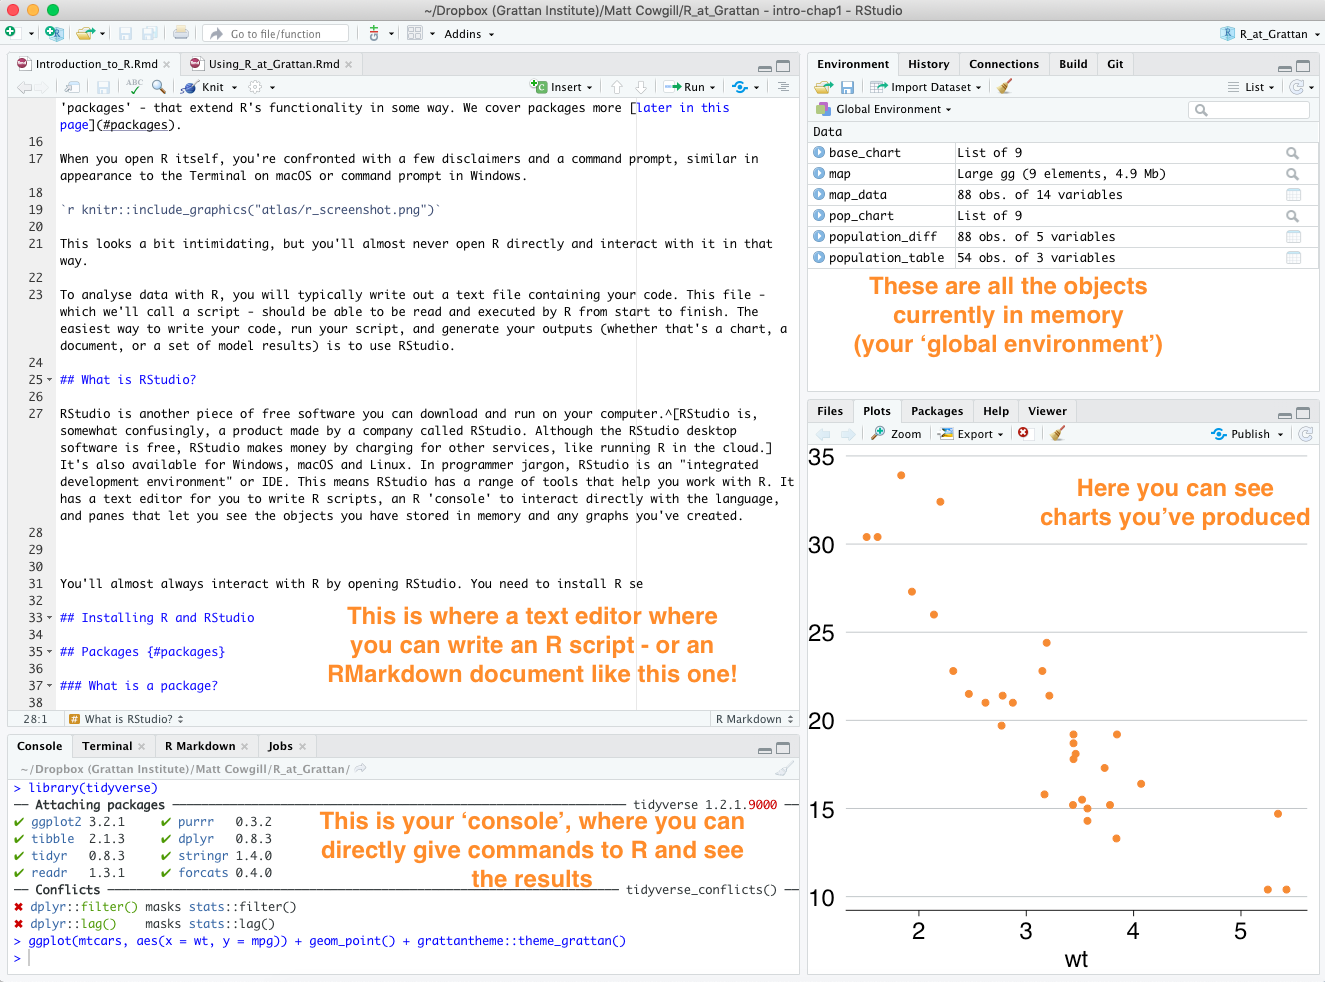
\includegraphics[width=18.4in]{atlas/rstudio_screenshot}

You'll almost always interact with R by opening RStudio.

\hypertarget{installing-r-and-rstudio}{%
\section{Installing R and RStudio}\label{installing-r-and-rstudio}}

Although you'll usually work with R by opening RStudio, you need to install both R and RStudio separately.

Install R by going to \href{https://cran.r-project.org}{CRAN}, the Comprehensive R Archive Network. CRAN is a community-run website that houses R itself as well as a broad range of R packages.

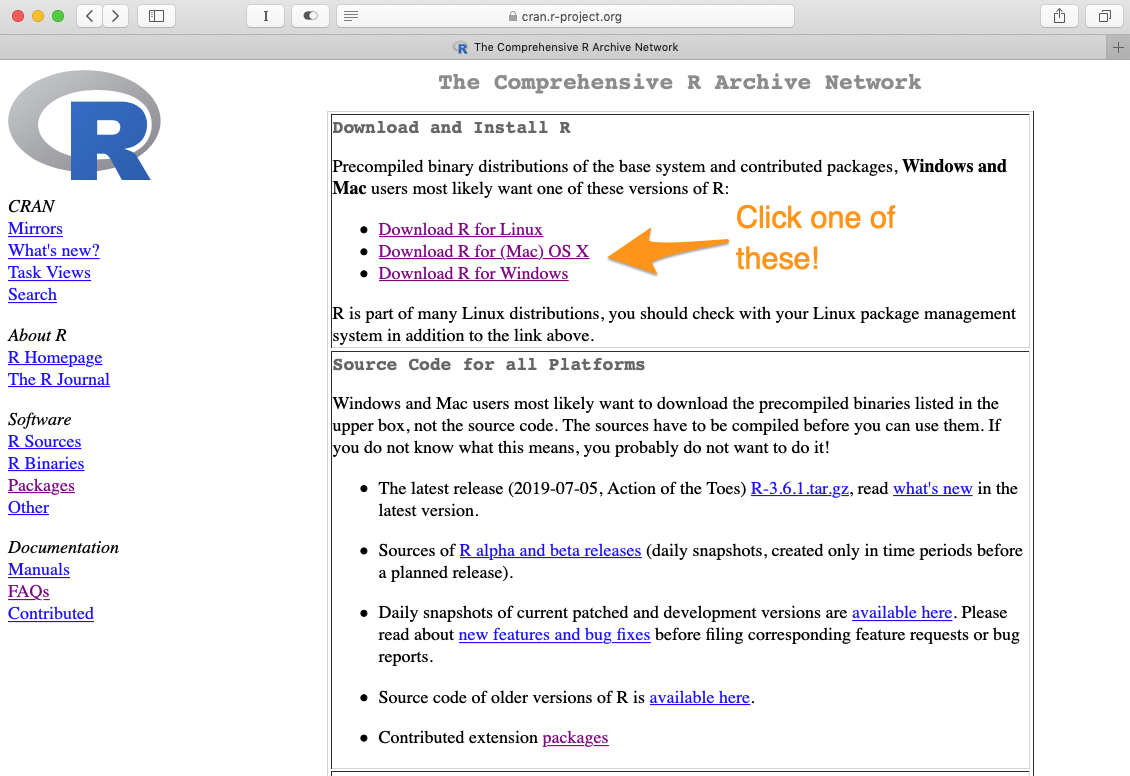
\includegraphics[width=15.69in]{atlas/r_cran}

You want to download the latest base R release, as a `binary'. Don't worry, you don't need to know what a binary is.

For macOS, the page will look like this:

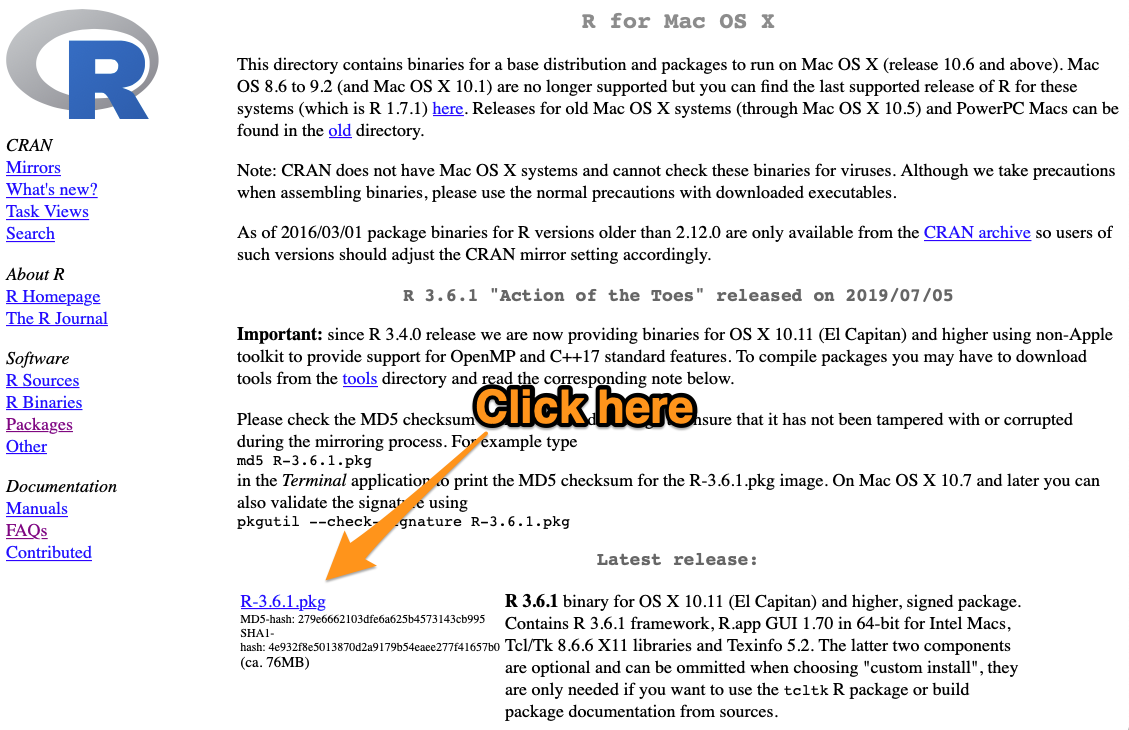
\includegraphics[width=15.68in]{atlas/r_cran_macos}

For Windows, you'll need to click on the `base' version, and then click again to start the download.

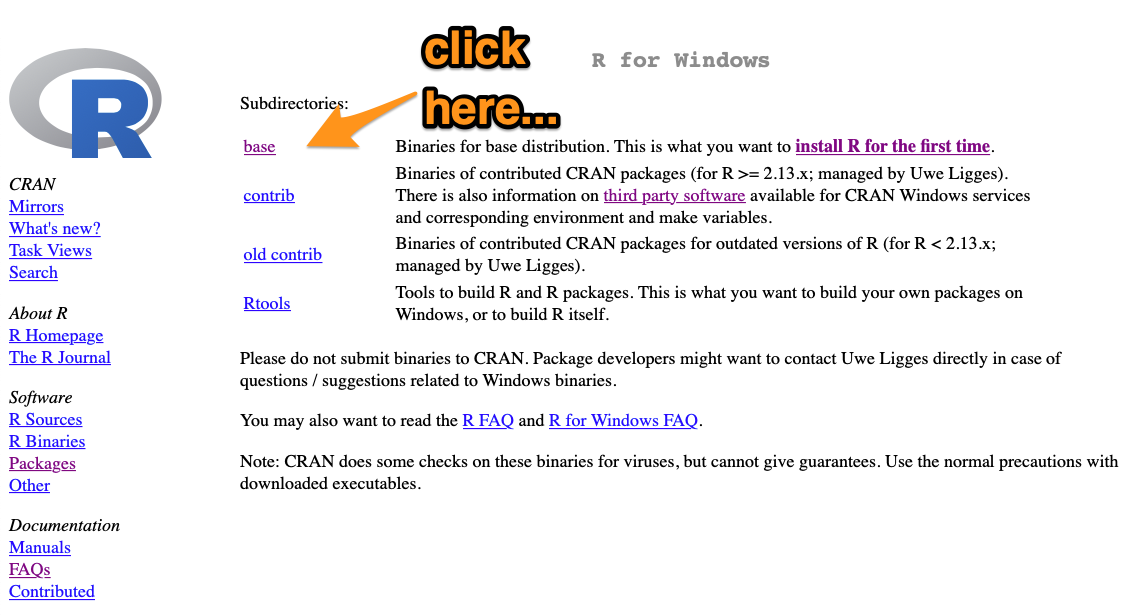
\includegraphics[width=15.69in]{atlas/r_cran_windows_1}
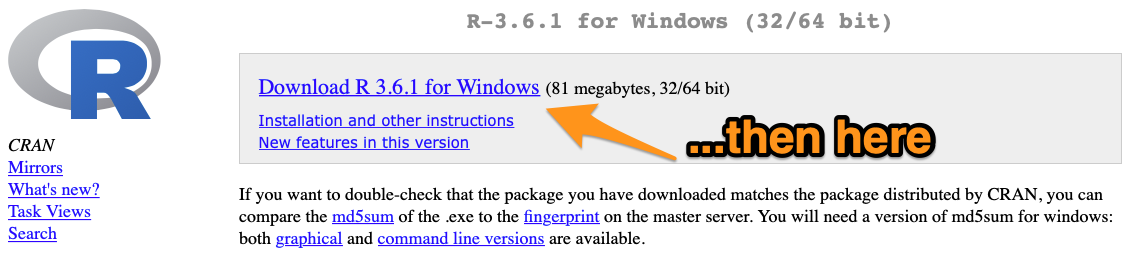
\includegraphics[width=15.67in]{atlas/r_cran_windows_2}

Once you've installed R, you'll need to install RStudio. Go to the \href{https://www.rstudio.com/products/rstudio/download/\#download}{RStudio website and install the latest version} of RStudio Desktop (open source license).

Once they're both installed, get started by opening RStudio.

\hypertarget{learning-more-about-r}{%
\section{Learning more about R}\label{learning-more-about-r}}

This guide will show you how to use R at Grattan. But it is not a comprehensive tool for learning R. The book \href{https://r4ds.had.co.nz}{R For Data Science} by Garrett Grolemund and Hadley Wickham is a great resource that will help you go from being a beginner to being able to do real-world analysis. The book is available for free online.

\hypertarget{why-use-r}{%
\chapter{Why use R?}\label{why-use-r}}

We can break this question into two parts:

\begin{enumerate}
\def\labelenumi{\arabic{enumi}.}
\tightlist
\item
  Why use script-based software to analyse data?
\item
  Why use R, specifically?
\end{enumerate}

\hypertarget{why-script}{%
\section{Why use script-based software?}\label{why-script}}

It's important for our analyses to be \textbf{reproducible}. This means that all of the steps that were taken to go from your raw data to your final outputs are clearly set out and can be reproduced if necessary.

Reproducibility is very important for quality control (``QC''), particularly of complex analyses - if it's not clear what you've done, it's hard for someone to check your work. It also makes things easier for you in the future - coming back to an old analysis a few months or years down the track is much easier if it's reproducible.

Script-based analyses are more likely to be reproducible.\footnote{Using a script-based approach doesn't guarantee that your analysis will be truly reproducible. If your work involves some steps that aren't documented in the script - such as data ``cleaning'' in Excel - then it is not fully reproducible.} A script sets out all the steps that were taken from reading in data, to tidying it, to estimating models or summary statistics and generating output.

Analysis that isn't script based, like work done in Excel, is almost never reproducible. It is generally unclear what steps were taken, in which order, to go from the raw data to the output. It isn't even always clear in a spreadsheet what is the `raw data' and what has been modified in some way.

Using scripts makes us less susceptible to the sort of errors \href{https://en.wikipedia.org/wiki/Growth_in_a_Time_of_Debt\#Methodological_flaws}{famously made by the economists Reinhart and Rogoff} in their Excel-based analysis of the effect of public debt on economic growth. It's still quite possible to make errors in a script-based analysis, but those errors are easier to find when the analysis is more transparent.

Script-based analysis software also allows us to:
* Work with larger data sets;
* Work with data in a broader range of formats;
* Easily combine different data sets;
* Automate tasks and build from previous analyses; and
* Estimate a broad range of statistical models.

\hypertarget{why-R}{%
\section{Why use R specifically?}\label{why-R}}

Doing reproducible, script-based, research doesn't necessarily involve using R. It's perfectly possible to do reproducible work in Stata or Python (though somewhat harder in SPSS, where data is primarily manipulated by clicking things).

We use R specifically because:
* It's free!
* It's open source.
* It's powerful, particularly when it comes to statistics and data science.
* It's flexible and customisable.
* It has an active community extending its capabilities all the time and providing support online.
* It is becoming the norm in academic research and common in the corporate world.

Everything you can do in Excel can, and usually should, be done in R.

\hypertarget{part-using-r-the-grattan-way}{%
\part{Using R the Grattan way}\label{part-using-r-the-grattan-way}}

\hypertarget{organising-projects}{%
\chapter{Organising an R project at Grattan}\label{organising-projects}}

All our work at Grattan, whether it's in R or some other software, should heed the ``hit by a bus'' rule. If you're not around, colleagues should be able to access, understand, verify, and build on the work you've done.

Organising your analysis in a predictable, consistent way helps to make your work reproducible by others, including yourself in the future. This is really important! If your analysis is messy, you're more likely to make errors, and less likely to spot them. Other people will find it hard to check your analysis and you'll find it harder to return to it down the track.

This page sets out some guidelines for organising your work in R at Grattan. It covers:

\begin{itemize}
\tightlist
\item
  Using RStudio projects and relative filepaths;
\item
  Using a consistent subfolder structure; and
\item
  Naming your scripts and keeping them manageable.
\end{itemize}

Using a consistent coding style also helps make our work more shareable; that's \protect\hyperlink{coding-style}{covered on the next page}.

\hypertarget{use-rstudio-projects-not-setwd}{%
\section{\texorpdfstring{Use RStudio projects, not \texttt{setwd()}}{Use RStudio projects, not setwd()}}\label{use-rstudio-projects-not-setwd}}

In Excel, your data, code and output generally all live together in one file. In R, you have a script, which will usually load some data, do something to it, and save some output. You end up with multiple files - the raw data, your script, and some output.

When it's executing your script, R needs to know where to read files from and save files to. By default, it uses your working directory. Your working directory is shown at the top of your console in RStudio, or you can find out what it is by running the command \texttt{getwd()}.

You can tell R which folder to use as your working directory by using the command \texttt{setwd()}, as in \texttt{setwd("\textasciitilde{}/Desktop/some\ random\ folder")} or \texttt{setwd("C:\textbackslash{}Users\textbackslash{}mcowgill\textbackslash{}Documents\textbackslash{}Somerandomfolder")}. \textbf{This is a bad idea that you should avoid!} If anyone - including you - tries to run your script on a different machine, with a different folder structure, it probably won't work. If people can't get past the first line when they're trying to run your script, there's an annoying and unnecessary hurdle to reproducing and checking your analysis.

In the \href{https://www.tidyverse.org/articles/2017/12/workflow-vs-script/}{words of Jenny Bryan}:

\begin{quote}
if the first line of your R script is \texttt{setwd("C:\textbackslash{}Users\textbackslash{}jenny\textbackslash{}path\textbackslash{}that\textbackslash{}only\textbackslash{}I\textbackslash{}have")} I will come into your office and SET YOUR COMPUTER ON FIRE.
\end{quote}

Seems fair.

Creating a `project' in RStudio sets your working directory in a way that's portable across machines. Creating an RStudio project is straightforward: \textbf{click File, then New Project}. You can then choose to start your project in a new directory, or an existing directory. Simple!

\begin{center}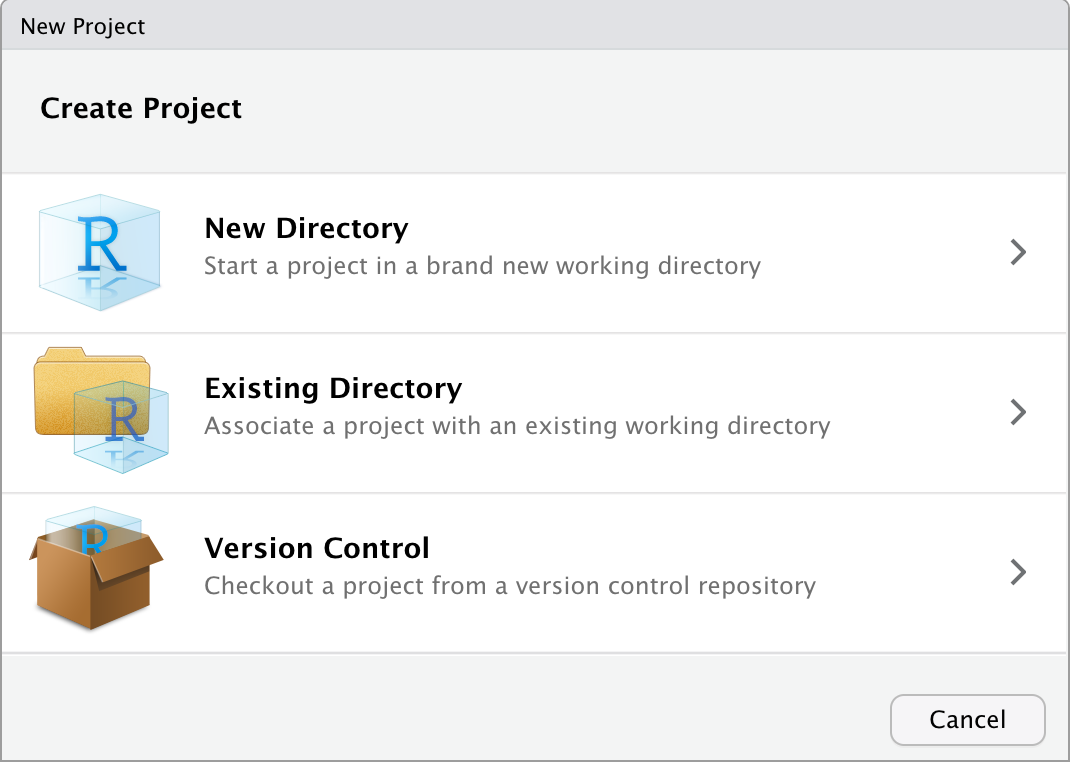
\includegraphics[width=0.66\linewidth]{atlas/rstudio_newproject} \end{center}

RStudio will then create a file with an .Rproj extension in the folder you've chosen. When you want to work in this project, just open the .Rproj file, or click File -\textgreater{} Open project in RStudio. Your working directory will be set to the directory that contains the .Rproj file.

\hypertarget{use-relative-filepaths}{%
\section{Use relative filepaths}\label{use-relative-filepaths}}

A benefit of using RStudio projects is that you can use relative filepaths rather than machine-specific filepaths.
Machine-specific filepaths not only stop you from sharing your work with others, they're also super annoying for! Who wants to type out a full filepath everytime you load or save a file?

\textbf{Bad, machine-specific filepaths}

\begin{Shaded}
\begin{Highlighting}[]
\NormalTok{hes <-}\StringTok{ }\KeywordTok{read_csv}\NormalTok{(}\StringTok{"/Users/mcowgill/Desktop/hes1516.csv"}\NormalTok{)}
\NormalTok{hes <-}\StringTok{ }\KeywordTok{read_csb}\NormalTok{(}\StringTok{"C:\textbackslash{}Users\textbackslash{}mcowgill\textbackslash{}Desktop\textbackslash{}hes1516.csv"}\NormalTok{)}
\KeywordTok{grattan_save}\NormalTok{(}\StringTok{"/Users/mcowgill/Desktop/images/expenditure_by_income.pdf"}\NormalTok{)}
\end{Highlighting}
\end{Shaded}

Instead, use relative filepaths. These are filepaths that are relative (hence the name) to your project folder, which you set by creating an RStudio project.

\textbf{Good, relative filepaths}

\begin{Shaded}
\begin{Highlighting}[]
\NormalTok{hes <-}\StringTok{ }\KeywordTok{read_csv}\NormalTok{(}\StringTok{"data/HES/hes1516.csv"}\NormalTok{)}
\KeywordTok{grattan_save}\NormalTok{(}\StringTok{"atlas/expenditure_by_income.pdf"}\NormalTok{)}
\end{Highlighting}
\end{Shaded}

The first example above tells R to look in the `data' subdirectory of your project folder, and then the `HES' subdirectory of `data', to find the `hes1516.csv' file. This file path isn't specific to your machine, so your code is more shareable this way.

\hypertarget{keep-your-stuff-together}{%
\section{Keep your stuff together}\label{keep-your-stuff-together}}

Your script(s), data, and output should generally all live in the same place. \footnote{This isn't always possible, like when you're working with restricted-access microdata. But unless there's a really good reason why you can't keep your data together with the rest of your work, you should do it.} That place should be the folder that contains the .Rproj file that was created when you created an RStudio project, and subfolders of that folder.

Don't just put everything in your project folder itself. This can get really overwhelming and confusing, particularly for anyone trying to understand and check your work. Instead, separate your code, your source data, and your output into subfolders.

A good structure is to have a subfolder for:

\begin{itemize}
\tightlist
\item
  your code - called `R'
\item
  your source data - called `data'
\item
  your graphs - called `atlas', like in our LaTeX projects
\item
  your non-graph output, like formatted tables, called `output'
\end{itemize}

Sometimes your data folder might have subfolders - `raw' for data that you've done nothing to, and `clean' for data you've modified in some way.\footnote{Other folder structures are OK and might make more sense for your project. The important thing is to \textbf{have} a folder structure, and to use a structure that is easily comprehensible to anyone else looking at your analysis.} Don't keep `raw' data together in the same place as data you've modified.

\hypertarget{manageable}{%
\section{Keep your scripts manageable}\label{manageable}}

Unless your project is very simple, it's probably not a good idea to put all your work into one R script. Instead, break your analysis into discrete pieces and put each piece in its own file. Number the files to make it clear what order they're supposed to be run in.

Here's a useful structure:

\begin{itemize}
\tightlist
\item
  01\_import.R
\item
  02\_tidy.R
\item
  03\_model.R
\item
  04\_visualise.R
\end{itemize}

It should be clear what each script is trying to do. Use meaningful filenames that clearly indicate the overarching purpose of the script. Use comments to explain why you're doing things. Err on the side of over-commenting, rather than under-commenting (we cover this more \protect\hyperlink{use-comments}{elsewhere in this guide}).

\hypertarget{README}{%
\section{Include a README file}\label{README}}

Your analysis workflow might seem completely obvious to you. Let's say that in one script you load raw ABS microdata, run a particular script to clean it up, save the cleaned data somewhere, then load that cleaned data in a second script to produce a summary table, then use a third script to produce a graph based on the summary table. Easy!

Except that might not seem easy or self-explanatory to anyone who comes along and tries to figure out how your analysis works, including you in the future.

Make things easier by including a short text file - called README - in the project folder. This should explain the purpose of the project, the key files, and (if it isn't clear) the order in which they should be run. If you got the data from somewhere non-obvious, explain that in the README file.

\hypertarget{omit-needless-code}{%
\section{Omit needless code}\label{omit-needless-code}}

Don't retain code that ultimately didn't lead anywhere. If you produced a graph that ended up not being used, don't keep the code in your script - if you want to save it, move it to a subfolder named `archive' or similar. Your code should include the steps needed to go from your raw data to your output - and not extraneous steps. If you ask someone to QC your work, they shouldn't have to wade through 1000 lines of code just to find the 200 lines that are actually required to produce your output.

When you're doing data analysis, you'll often give R interactive commands to help you understand what your data looks like. For example, you might view a dataframe with \texttt{View(mydf)} or \texttt{str(mydf)}. This is fine, and often necessary, when you're doing your analysis. \textbf{Don't keep these commands in your script}. These type of commands should usually be entered straight into the R console, not in a script. If they're in your script, delete them.

\hypertarget{rules_9a_final_final_mc}{%
\section{Rules\_9a\_FINAL\_FINAL\_MC}\label{rules_9a_final_final_mc}}

We're all familiar with this hellish scenario: you do some work in a Word document (shudder, shudder, the horror, etc.), email it to a colleague, the colleague edits it and sends it back with a tweaked filename, like \texttt{cool\_word\_doc\_002.docx}. Try to avoid replicating this nightmare in R.

\textbf{Don't} create multiple versions of the same script (like \texttt{analysis\_FINAL\_002\_MC.R} and \texttt{analysis\_FINALFINAL\_003\_MC\_WM.R}.) If you do end up with multiple versions, put everything other than the latest version in a subfolder of your ``R'' folder, called ``R/archive''. To avoid a horrible mess of \texttt{analysis\_FINAL\_002.R} type documents cluttering up your folder, consider using \protect\hyperlink{version-control}{Git for version control}.

\hypertarget{coding-style}{%
\chapter{Grattan coding style}\label{coding-style}}

The benefits of a common coding style are well explained \href{http://r-pkgs.had.co.nz/style.html}{by Hadley Wickham}:

\begin{quote}
Good style is important because while your code only has one author, it'll usually have multiple readers. This is especially true when you're writing code with others. In that case, it's a good idea to agree on a common style up-front.
\end{quote}

Below we describe the \textbf{key} elements of Grattan coding style, without being too tedious about it all. There are many elements of coding style we don't cover in this guide; if you're unsure about anything, \href{https://style.tidyverse.org/}{consult the \texttt{tidyverse} guide}.

You should also see the \protect\hyperlink{organising-projects}{Using R at Grattan} page for guidelines about setting up projects.

\hypertarget{script-preamble}{%
\section{Script preamble}\label{script-preamble}}

Describe what your script does in the first few lines using comments or within an RMarkdown document.

\textbf{Good}

\begin{Shaded}
\begin{Highlighting}[]
\CommentTok{# This script reads ABS data downloaded from TableBuilder and combines into a single data object containing post-secondary education levels by age and gender by SA3. }
\end{Highlighting}
\end{Shaded}

Your preamble might also pose a research question that the script will answer.

\textbf{Good}

\begin{Shaded}
\begin{Highlighting}[]
\CommentTok{# Do women have higher levels of educational attainment than men, within the same geographical areas and age groups?}
\end{Highlighting}
\end{Shaded}

Your preamble shouldn't be a terse, inscrutable comment.

\textbf{Bad}

\begin{Shaded}
\begin{Highlighting}[]
\CommentTok{# make ABS ed data graph}
\end{Highlighting}
\end{Shaded}

If it's hard to concisely describe what your script does in a few lines of plain English, that might be a sign that your script does too many things. Consider breaking your analysis into a series of scripts. See \protect\hyperlink{organising-projects}{Organising R Projects at Grattan} for more.

Your preamble should anticipate and answer any questions other people might have when reviewing your script. For example:

\textbf{Good}

\begin{Shaded}
\begin{Highlighting}[]
\CommentTok{# This script calculates average income by age group and sex using the ABS Household Expenditure Survey and joins this to health information by age groups and sex from the National Health Survey. Note that we can't use the income variable in the NHS for this purpose, as it only contains information about respondents' income decile, not the income itself.}
\end{Highlighting}
\end{Shaded}

The preamble should pertain the the code contained in the specific script. If you have comments or information about your analysis as a whole, put it in your \protect\hyperlink{README}{README file}.

\hypertarget{use-comments}{%
\section{Use comments}\label{use-comments}}

Comments are necessary where the code \emph{alone} doesn't tell the full story. Comments should tell the reader \textbf{why} you're doing something, rather than just \textbf{what} you're doing.

For example, comments are important when groups are coded with numbers rather than character strings, because this might not be obvious to someone reading your script:

\textbf{Necessary to comment}

\begin{Shaded}
\begin{Highlighting}[]
\NormalTok{data }\OperatorTok\StringTok{ }
\StringTok{  }\KeywordTok{filter}\NormalTok{(gender }\OperatorTok{==}\StringTok{ }\DecValTok{1}\NormalTok{,   }\CommentTok{# Keep only male observations}
\NormalTok{         age }\OperatorTok{==}\StringTok{ "05"}\NormalTok{)   }\CommentTok{# Keep only 35-39 year-olds. }
\end{Highlighting}
\end{Shaded}

Without the comment, readers of your code might not be aware that \texttt{1} in this dataset corresponds to \texttt{male}, or that \texttt{age\ ==\ "05"} refers to 35-39 year olds. Without the comment, the code is not self-explanatory.

If your code \emph{is} self-explanatory, you can include or omit comments as you see fit.

\textbf{Not necessary (but okay if included)}

\begin{Shaded}
\begin{Highlighting}[]
\CommentTok{# We want to only look at women aged 35-39}
\NormalTok{data }\OperatorTok\StringTok{ }
\StringTok{  }\KeywordTok{filter}\NormalTok{(gender }\OperatorTok{==}\StringTok{ "Female"}\NormalTok{,}
\NormalTok{         age }\OperatorTok{>=}\StringTok{ }\DecValTok{35} \OperatorTok{&}\StringTok{ }\NormalTok{age }\OperatorTok{<=}\StringTok{ }\DecValTok{39}\NormalTok{)}
\end{Highlighting}
\end{Shaded}

You should also include comments where your code is more complex and may not be easily understood by the reader. If you're using a function from a package that isn't commonly used at Grattan, include a comment to explain what it does.

\emph{Err on the side of commenting more}, rather than less, throughout your code. Something may seem obvious to you when you're writing your code, but it might not be obvious to the person reading your code, even if that person is you in the future. Better to over-comment than under-comment.

Comments can go above code chunks, or next to code - there are examples of both above.

\hypertarget{breaking-your-script-into-chunks}{%
\section{Breaking your script into chunks}\label{breaking-your-script-into-chunks}}

It's useful to break a lengthy script into chunks with \texttt{-\/-\/-\/-\/-}.

\textbf{Good}

\begin{Shaded}
\begin{Highlighting}[]
\CommentTok{# Read file A -----}

\NormalTok{a <-}\StringTok{ }\KeywordTok{read_csv}\NormalTok{(}\StringTok{"data/a.csv"}\NormalTok{)}

\CommentTok{# Read file B -----}

\NormalTok{b <-}\StringTok{ }\KeywordTok{read_csv}\NormalTok{(}\StringTok{"data/b.csv"}\NormalTok{)}

\CommentTok{# Combine files A and B ----}

\NormalTok{c <-}\StringTok{ }\KeywordTok{bind_rows}\NormalTok{(a, b)}
\end{Highlighting}
\end{Shaded}

This helps you, and others, navigate your code better, using the navigation tool built in to RStudio. In the script editor pane of RStudio, at the bottom left, there's a little navigation tool that helps you easily jump between named sections of your script.

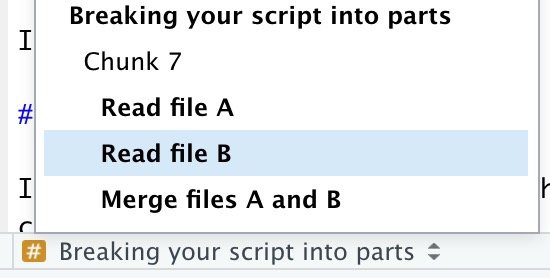
\includegraphics[width=7.64in]{atlas/rstudio_navigation}

Breaking your script into chunks with \texttt{-\/-\/-\/-\/-} also makes your code easier to read.

\hypertarget{assigning-values-to-objects}{%
\section{Assigning values to objects}\label{assigning-values-to-objects}}

In R, you work with objects. An object might be a data frame, or a vector of numbers or letters, or a list. Functions can be objects, too.

\textbf{Use the \texttt{\textless{}-} operator to assign values to objects}. Here are some \textbf{good} examples:

\begin{Shaded}
\begin{Highlighting}[]
\NormalTok{schools <-}\StringTok{ }\KeywordTok{read_csv}\NormalTok{(}\StringTok{"data/schools_data.csv"}\NormalTok{)}

\NormalTok{three_letters <-}\StringTok{ }\KeywordTok{c}\NormalTok{(}\StringTok{"a"}\NormalTok{, }\StringTok{"b"}\NormalTok{, }\StringTok{"c"}\NormalTok{)}

\NormalTok{lf <-}\StringTok{ }\NormalTok{labour_force }\OperatorTok
\StringTok{  }\KeywordTok{filter}\NormalTok{(status }\OperatorTok{!=}\StringTok{ "NILF"}\NormalTok{)}
\end{Highlighting}
\end{Shaded}

Avoid \texttt{-\textgreater{}}, \texttt{=} and \texttt{assign()}. Here are some \textbf{bad} examples::

\begin{Shaded}
\begin{Highlighting}[]
\NormalTok{schools =}\StringTok{ }\KeywordTok{read_csv}\NormalTok{(}\StringTok{"data/schools_data.csv"}\NormalTok{)}

\KeywordTok{assign}\NormalTok{(}\StringTok{"three_letters"}\NormalTok{, }\KeywordTok{c}\NormalTok{(}\StringTok{"a"}\NormalTok{, }\StringTok{"b"}\NormalTok{, }\StringTok{"c"}\NormalTok{))}

\NormalTok{labour_force }\OperatorTok
\StringTok{  }\KeywordTok{filter}\NormalTok{(status }\OperatorTok{!=}\StringTok{ "NILF"}\NormalTok{) ->}\StringTok{ }\NormalTok{lf}
\end{Highlighting}
\end{Shaded}

All these bad operators will work, but they are best avoided. The \texttt{=} operator is avoided for reasons of visual consistency, style, and to avoid confusion. \texttt{assign()} is avoided because it can lead to unexpected behaviour, and is usually not the best way to do what you want to do. The \texttt{-\textgreater{}} operator is avoided because it's easy to miss when skimming over code.

The \texttt{\textless{}\textless{}-} operator should also be avoided.

\hypertarget{naming-objects-and-variables}{%
\section{Naming objects and variables}\label{naming-objects-and-variables}}

It's important to be consistent when naming things. This saves you time when writing code. If you use a consistent naming convention, you don't need to stop to remember if your object is called \texttt{ed\_by\_age} or \texttt{edByAge} or \texttt{ed.by.age}. Having a consistent naming convention across Grattan also makes it easy to read and QC each other's code.

Grattan primarily uses \emph{words separated by underscores} \texttt{\_} (aka `snake\_case') to name objects and variables. This is \href{https://style.tidyverse.org/syntax.html\#object-names}{considered good practice across the Tidyverse}.
Object names should be descriptive and not-too-long. This is a trade-off, and one that's sometimes hard to get right. However, using snake\_case provides consistency:

\textbf{Good object names}

\begin{Shaded}
\begin{Highlighting}[]
\NormalTok{sa3_population}
\NormalTok{gdp_growth_vic}
\NormalTok{uni_attainment}
\end{Highlighting}
\end{Shaded}

\textbf{Bad object names}

\begin{Shaded}
\begin{Highlighting}[]
\NormalTok{sa3Pop}
\NormalTok{GDPgrowthVIC}
\NormalTok{uni.attainment}
\end{Highlighting}
\end{Shaded}

Variable names face a similar trade-off. Again, try to be descriptive and short using snake\_case:

\textbf{Good variable names}

\begin{Shaded}
\begin{Highlighting}[]
\NormalTok{gender}
\NormalTok{gdp_growth}
\NormalTok{highest_edu}
\end{Highlighting}
\end{Shaded}

\textbf{Bad variable names}

\begin{Shaded}
\begin{Highlighting}[]
\NormalTok{s801LHSAA}
\NormalTok{gdp.growth}
\NormalTok{highEdu}
\NormalTok{chaosVar_name.silly}
\NormalTok{var2}
\end{Highlighting}
\end{Shaded}

When you load data from outside Grattan, such as ABS microdata, variables will often have bad names. It is worth taking the time at the top of your script to \href{https://dplyr.tidyverse.org/reference/select.html}{rename your variables}, giving them consistent, descriptive, short, snake\_case names.

The most important thing is that your code is internally consistent - you should stick to one naming convention for all your objects and variables. Using snake\_case, which we strongly recommend, reduces friction for other people reading and editing your code. Using short names saves effort when coding. Using descriptive names makes your code easier to read and understand.

\hypertarget{spacing}{%
\section{Spacing}\label{spacing}}

Giving your code room to breathe greatly helps readability for future-you and others who will have to read your code. Code without ample whitespace is hard to read, justasitishardertoreadEnglishsentenceswithoutspaces.

\hypertarget{assign-and-equals}{%
\subsection{Assign and equals}\label{assign-and-equals}}

Put a space each side of an assign operator \texttt{\textless{}-}, equals \texttt{=}, and other `infix operators' (\texttt{==}, \texttt{+}, \texttt{-}, and so on).

\textbf{Good}

\begin{Shaded}
\begin{Highlighting}[]
\NormalTok{uni_attainment <-}\StringTok{ }\KeywordTok{filter}\NormalTok{(data, age }\OperatorTok{==}\StringTok{ }\DecValTok{25}\NormalTok{, gender }\OperatorTok{==}\StringTok{ "Female"}\NormalTok{)}
\end{Highlighting}
\end{Shaded}

\textbf{Bad}

\begin{Shaded}
\begin{Highlighting}[]
\NormalTok{uni_attainment<-}\KeywordTok{filter}\NormalTok{(data,age}\OperatorTok{==}\DecValTok{25}\NormalTok{,gender}\OperatorTok{==}\StringTok{"Female"}\NormalTok{)}
\end{Highlighting}
\end{Shaded}

Exceptions are operators that \emph{directly connect} to an object, package or function, which should \textbf{not} have spaces on either side: \texttt{::}, \texttt{\$}, \texttt{@}, \texttt{{[}}, \texttt{{[}{[}}, etc.

\textbf{Good}

\begin{Shaded}
\begin{Highlighting}[]
\NormalTok{uni_attainment}\OperatorTok{$}\NormalTok{gender}
\NormalTok{uni_attainment}\OperatorTok{$}\NormalTok{age[}\DecValTok{1}\OperatorTok{:}\DecValTok{10}\NormalTok{]}
\NormalTok{readabs}\OperatorTok{::}\KeywordTok{read_abs}\NormalTok{()}
\end{Highlighting}
\end{Shaded}

\textbf{Bad}

\begin{Shaded}
\begin{Highlighting}[]
\NormalTok{uni_attainment }\OperatorTok{$}\StringTok{ }\NormalTok{gender}
\NormalTok{uni_attainment}\OperatorTok{$}\StringTok{ }\NormalTok{age [ }\DecValTok{1} \OperatorTok{:}\StringTok{ }\DecValTok{10}\NormalTok{]}
\NormalTok{readabs }\OperatorTok{::}\StringTok{ }\KeywordTok{read_abs}\NormalTok{()}
\end{Highlighting}
\end{Shaded}

\hypertarget{commas}{%
\subsection{Commas}\label{commas}}

Always put a space \emph{after} a comma and not before, just like in regular English.

\textbf{Good}

\begin{Shaded}
\begin{Highlighting}[]
\KeywordTok{select}\NormalTok{(data, age, gender, sa2, sa3)}
\end{Highlighting}
\end{Shaded}

\textbf{Bad}

\begin{Shaded}
\begin{Highlighting}[]
\KeywordTok{select}\NormalTok{(data,age,gender,sa2,sa3)}
\end{Highlighting}
\end{Shaded}

\hypertarget{parentheses}{%
\subsection{Parentheses}\label{parentheses}}

Do not use spaces around parentheses in most cases:

\textbf{Good}

\begin{Shaded}
\begin{Highlighting}[]
\KeywordTok{mean}\NormalTok{(x, }\DataTypeTok{na.rm =} \OtherTok{TRUE}\NormalTok{)}
\end{Highlighting}
\end{Shaded}

\textbf{Bad}

\begin{Shaded}
\begin{Highlighting}[]
\KeywordTok{mean}\NormalTok{ (x, }\DataTypeTok{na.rm =} \OtherTok{TRUE}\NormalTok{)}
\KeywordTok{mean}\NormalTok{( x, }\DataTypeTok{na.rm =} \OtherTok{TRUE}\NormalTok{ )}
\end{Highlighting}
\end{Shaded}

For spacing rules around \texttt{if}, \texttt{for}, \texttt{while}, and \texttt{function}, see \href{https://style.tidyverse.org/syntax.html\#parentheses}{the Tidyverse guide}.

\hypertarget{short-lines-and-line-indentation}{%
\section{Short lines and line indentation}\label{short-lines-and-line-indentation}}

It's tedious -- yes -- but short lines and consistent line indentation can help make reading code much easier. If you are supplying multiple arguments to a function, it's generally a good idea to put each argument on a new line - hit return after the comma, like in the \texttt{rename} and \texttt{filter} examples below. Indentation makes it clear where a code block starts and finishes.

Using pipes (\texttt{\%\textgreater{}\%}) instead of nesting functions also makes things clearer.{[}\^{}The pipe is from the \texttt{magrittr} package and is used to chain functions together, so that the output from one function becomes the input to the next function. The pipe is loaded as part of the \protect\hyperlink{tidyverse}{\texttt{tidyverse}}.{]} The pipe should always have a space before it, and should generally be followed by a new line, as in this example:

\textbf{Good: short lines and indentation}

\begin{Shaded}
\begin{Highlighting}[]
\NormalTok{young_qual_income <-}\StringTok{ }\NormalTok{data }\OperatorTok
\StringTok{  }\KeywordTok{rename}\NormalTok{(}\DataTypeTok{gender =}\NormalTok{ s801LHSAA,}
         \DataTypeTok{uni_attainment =}\NormalTok{ high.ed) }\OperatorTok
\StringTok{  }\KeywordTok{filter}\NormalTok{(income }\OperatorTok{>}\StringTok{ }\DecValTok{0}\NormalTok{,}
\NormalTok{         age }\OperatorTok{>=}\StringTok{ }\DecValTok{25} \OperatorTok{&}\StringTok{ }\NormalTok{age }\OperatorTok{<=}\StringTok{ }\DecValTok{34}\NormalTok{) }\OperatorTok
\StringTok{  }\KeywordTok{group_by}\NormalTok{(gender, uni_attainment) }\OperatorTok
\StringTok{  }\KeywordTok{summarise}\NormalTok{(}\DataTypeTok{mean_income =} \KeywordTok{mean}\NormalTok{(income, }\DataTypeTok{na.rm =} \OtherTok{TRUE}\NormalTok{))}
\end{Highlighting}
\end{Shaded}

Without indentation, the code is harder to read. It's not clear where the chunk starts and finishes, and which bits of code are arguments to which functions.

\textbf{Bad: short lines, no indentation}

\begin{Shaded}
\begin{Highlighting}[]
\NormalTok{young_qual_income <-}\StringTok{ }\NormalTok{data }\OperatorTok\StringTok{ }
\KeywordTok{rename}\NormalTok{(}\DataTypeTok{gender =}\NormalTok{ s801LHSAA,}
\DataTypeTok{uni_attainment =}\NormalTok{ high.ed) }\OperatorTok\StringTok{ }
\KeywordTok{filter}\NormalTok{(income }\OperatorTok{>}\StringTok{ }\DecValTok{0}\NormalTok{,}
\NormalTok{age }\OperatorTok{>=}\StringTok{ }\DecValTok{25} \OperatorTok{&}\StringTok{ }\NormalTok{age }\OperatorTok{<=}\StringTok{ }\DecValTok{34}\NormalTok{) }\OperatorTok
\KeywordTok{group_by}\NormalTok{(gender, uni_attainment) }\OperatorTok\StringTok{ }
\KeywordTok{summarise}\NormalTok{(}\DataTypeTok{mean_income =} \KeywordTok{mean}\NormalTok{(income, }\DataTypeTok{na.rm =} \OtherTok{TRUE}\NormalTok{))}
\end{Highlighting}
\end{Shaded}

Long lines are also bad and hard to read.
\textbf{Bad: long lines}

\begin{Shaded}
\begin{Highlighting}[]
\NormalTok{young_qual_income <-}\StringTok{ }\NormalTok{data }\OperatorTok\StringTok{ }\KeywordTok{rename}\NormalTok{(}\DataTypeTok{gender =}\NormalTok{ s801LHSAA, }\DataTypeTok{uni_attainment =}\NormalTok{ high.ed) }\OperatorTok\StringTok{ }\KeywordTok{filter}\NormalTok{(income }\OperatorTok{>}\StringTok{ }\DecValTok{0}\NormalTok{, age }\OperatorTok{>=}\StringTok{ }\DecValTok{25} \OperatorTok{&}\StringTok{ }\NormalTok{age }\OperatorTok{<=}\StringTok{ }\DecValTok{34}\NormalTok{) }\OperatorTok\StringTok{ }\KeywordTok{group_by}\NormalTok{(gender, uni_attainment) }\OperatorTok\StringTok{ }\KeywordTok{summarise}\NormalTok{(}\DataTypeTok{mean_income =} \KeywordTok{mean}\NormalTok{(income, }\DataTypeTok{na.rm =} \OtherTok{TRUE}\NormalTok{))}
\end{Highlighting}
\end{Shaded}

When you want to take the output of a function and pass it as the input to another function, use the pipe (\texttt{\%\textgreater{}\%}). Don't write ugly, inscrutable code like this, where multiple functions are wrapped around other functions.

\textbf{War-crime bad: long lines without pipes}

\begin{Shaded}
\begin{Highlighting}[]
\NormalTok{young_qual_income<-}\KeywordTok{summarise}\NormalTok{(}\KeywordTok{group_by}\NormalTok{(}\KeywordTok{filter}\NormalTok{(}\KeywordTok{rename}\NormalTok{(data,}\DataTypeTok{gender=}\NormalTok{s801LHSAA,}\DataTypeTok{uni_attainment=}\NormalTok{high.ed),income}\OperatorTok{>}\DecValTok{0}\NormalTok{,age}\OperatorTok{>=}\DecValTok{25}\OperatorTok{&}\NormalTok{age}\OperatorTok{<=}\DecValTok{34}\NormalTok{),uni_attainment),}\DataTypeTok{mean_income=}\KeywordTok{mean}\NormalTok{(income,}\DataTypeTok{na.rm=}\OtherTok{TRUE}\NormalTok{))}
\end{Highlighting}
\end{Shaded}

Writing clear code chunks, where functions are strung together with a pipe (\texttt{\%\textgreater{}\%}), makes your code much more expressive and able to be read and understood. This is another reason to favour R over something like Excel, which pushes people to piece together functions into Frankenstein's monsters like this:

\begin{Shaded}
\begin{Highlighting}[]
\NormalTok{=}\KeywordTok{IF}\NormalTok{(}\OperatorTok{$}\DataTypeTok{G16 =} \StringTok{"All day"}\NormalTok{, }\KeywordTok{INDEX}\NormalTok{(metrics}\OperatorTok{!}\ErrorTok{$}\NormalTok{D}\OperatorTok{$}\DecValTok{8}\OperatorTok{:}\ErrorTok{$}\NormalTok{H}\OperatorTok{$}\DecValTok{66}\NormalTok{, }\KeywordTok{MATCH}\NormalTok{(}\KeywordTok{INDEX}\NormalTok{(correspondence}\OperatorTok{!}\ErrorTok{$}\NormalTok{B}\OperatorTok{$}\DecValTok{2}\OperatorTok{:}\ErrorTok{$}\NormalTok{B}\OperatorTok{$}\DecValTok{23}\NormalTok{, }\KeywordTok{MATCH}\NormalTok{(}\StringTok{'convert to tibble'}\OperatorTok{!}\NormalTok{M}\OperatorTok{$}\DecValTok{4}\NormalTok{, correspondence}\OperatorTok{!}\ErrorTok{$}\NormalTok{A}\OperatorTok{$}\DecValTok{2}\OperatorTok{:}\ErrorTok{$}\NormalTok{A}\OperatorTok{$}\DecValTok{23}\NormalTok{, }\DecValTok{0}\NormalTok{)), metrics}\OperatorTok{!}\ErrorTok{$}\NormalTok{B}\OperatorTok{$}\DecValTok{8}\OperatorTok{:}\ErrorTok{$}\NormalTok{B}\OperatorTok{$}\DecValTok{66}\NormalTok{, }\DecValTok{0}\NormalTok{), }\KeywordTok{MATCH}\NormalTok{(}\StringTok{'convert to tibble'}\OperatorTok{!}\ErrorTok{$}\NormalTok{E16, metrics}\OperatorTok{!}\ErrorTok{$}\NormalTok{D}\OperatorTok{$}\DecValTok{4}\OperatorTok{:}\ErrorTok{$}\NormalTok{H}\OperatorTok{$}\DecValTok{4}\NormalTok{, }\DecValTok{0}\NormalTok{)), }\StringTok{"NA"}\NormalTok{)}
\end{Highlighting}
\end{Shaded}

I just threw up in my mouth a little bit.

\hypertarget{blocks-of-code}{%
\section{Blocks of code}\label{blocks-of-code}}

As shown above, the pipe function \texttt{\%\textgreater{}\%} can make code more easy to write and read. The pipe can create the temptation to string together lots and lots of functions into one block of code. This can make things harder to read and understand.

Resist the urge to use the pipe to make code blocks too long. A block of code should generally do one thing, or a small number of things.

\hypertarget{packages-commonly-used-at-grattan}{%
\chapter{Packages commonly used at Grattan}\label{packages-commonly-used-at-grattan}}

R comes with a lot of functions - commands - built in to do a broad range of tasks. You could, if you really wanted, import a dataset, clean it up, estimate a model, and make a plot all using the functions that come with R - known as `base R'\footnote{Technically some of the `built-in' functions are part of packages, like the \texttt{tools}, \texttt{utils} and \texttt{stats} packages that come with R. We'll refer to all these as base R.}. Like R itself, packages are free and open source. You can install them from within RStudio.

Some packages - like the \texttt{tidyverse} collection of packages - are broadly popular among R users. Some - like the \texttt{grattantheme} package - are specific to Grattan Institute. Others - like the \texttt{readabs} package - are made by Grattan people, useful at Grattan, but also used outside of the Institute.

\hypertarget{install-packages}{%
\section{Installing packages}\label{install-packages}}

You'll typically install packages using the console in RStudio. That's the part of the window that, by default, sits in the bottom-left corner of the screen.

In our work at Grattan, we use packages from two different source: CRAN and Github. The main difference you need to know about is that we use different commands to install packages from these two sources.

To install a package from CRAN, we use the command \texttt{install.packages()}.

For example, this code will install the \texttt{ggplot2} package from CRAN:

\begin{Shaded}
\begin{Highlighting}[]
\KeywordTok{install.packages}\NormalTok{(}\StringTok{"ggplot2"}\NormalTok{)}
\end{Highlighting}
\end{Shaded}

The easiest way to install a package from Github is to use the function \texttt{install\_github()}. Unfortunately, this function doesn't come with base R. The \texttt{install\_github()} function is part of the \texttt{remotes} package. To use it, we first need to install \texttt{remotes} from CRAN:

\begin{Shaded}
\begin{Highlighting}[]
\KeywordTok{install.packages}\NormalTok{(}\StringTok{"remotes"}\NormalTok{)}
\end{Highlighting}
\end{Shaded}

Now we can install packages from Github using the \texttt{install\_github()} function from the \texttt{remotes} package. For example, here's how we would install the Grattan ggplot2 theme, which we'll discuss later in this website:

\begin{Shaded}
\begin{Highlighting}[]
\NormalTok{remotes}\OperatorTok{::}\KeywordTok{install_github}\NormalTok{(}\StringTok{"mattcowgill/grattantheme"}\NormalTok{, }\DataTypeTok{dependencies =} \OtherTok{TRUE}\NormalTok{, }\DataTypeTok{upgrade =} \StringTok{"always"}\NormalTok{)}
\end{Highlighting}
\end{Shaded}

\hypertarget{using-packages}{%
\section{Using packages}\label{using-packages}}

Before using a function that comes from a package, as opposed to base R, you need to tell R where to look for the function. There are two main ways to do that.

We can either load (aka `attach') the package by using the \texttt{library()} function. We typically do this at the top of a script.

\begin{Shaded}
\begin{Highlighting}[]
\KeywordTok{library}\NormalTok{(remotes)}

\CommentTok{# Now that the `remotes` package is loaded, we can use its `install_github()` function:}

\KeywordTok{install_github}\NormalTok{(}\StringTok{"mattcowgill/grattantheme"}\NormalTok{)}
\end{Highlighting}
\end{Shaded}

Or, we can use two colons - \texttt{::} - to tell R to use an individual function from a package without loading it:

\begin{Shaded}
\begin{Highlighting}[]
\NormalTok{remotes}\OperatorTok{::}\KeywordTok{install_github}\NormalTok{(}\StringTok{"mattcowgill/grattantheme"}\NormalTok{)}
\end{Highlighting}
\end{Shaded}

It usually makes sense to load a package with \texttt{library()}, unless you only need to use one of its function once or twice. There's no harm to using the \texttt{::} operator even if you have already loaded a package with \texttt{library()}. This can remove ambiguity both for R and for humans reading your code, particularly if you're using an obscure function - it makes it clearer where the function comes from.

\hypertarget{tidyverse}{%
\section{The tidyverse!}\label{tidyverse}}

The \texttt{tidyverse} is central to our work at Grattan. The \texttt{tidyverse} is a \href{https://www.tidyverse.org/packages/}{collection of related R packages} for importing, wrangling, exploring and visualising data in R. The packages are designed to work well together. You install the \texttt{tidyverse} in the \protect\hyperlink{install-packages}{usual way}:

\begin{Shaded}
\begin{Highlighting}[]
\KeywordTok{install.packages}\NormalTok{(}\StringTok{"tidyverse"}\NormalTok{)}
\end{Highlighting}
\end{Shaded}

The main packages in the \texttt{tidyverse} include:

\begin{itemize}
\tightlist
\item
  \emph{ggplot2} for making beautiful, customisable graphs
\item
  \emph{dplyr} for manipulating data frames
\item
  \emph{tidyr} for tidying your data
\item
  \emph{readr} for importing data from a broad range of formats
\item
  \emph{purrr} for functional programming
\item
  \emph{stringr} for manipulating strings of text
\end{itemize}

All these packages (and more!) will automatically be loaded for you when you run the command\footnote{There's no need to install or load the individual \texttt{tidyverse} packages - like \texttt{dplyr} - separately. Just install them all together, and load them with the single \texttt{library(tidyverse)} command. That way, you don't need to remember which functions come from \texttt{tidyr} and which from \texttt{dplyr} - they're all just \texttt{tidyverse} functions.}:

\begin{Shaded}
\begin{Highlighting}[]
\KeywordTok{library}\NormalTok{(tidyverse)}
\end{Highlighting}
\end{Shaded}

\begin{verbatim}
## -- Attaching packages ---------------------------------- tidyverse 1.2.1 --
\end{verbatim}

\begin{verbatim}
## v ggplot2 3.2.1     v purrr   0.3.3
## v tibble  2.1.3     v dplyr   0.8.3
## v tidyr   1.0.0     v stringr 1.4.0
## v readr   1.3.1     v forcats 0.4.0
\end{verbatim}

\begin{verbatim}
## -- Conflicts ------------------------------------- tidyverse_conflicts() --
## x dplyr::filter() masks stats::filter()
## x dplyr::lag()    masks stats::lag()
\end{verbatim}

A range of other packages are installed on your machine as part of the \texttt{tidyverse.} These include:

\begin{itemize}
\tightlist
\item
  \emph{readxl} for importing Excel spreadsheets into R
\item
  \emph{haven} for importing Stata, SAS and SPSS data
\item
  \emph{lubridate} for working with dates
\item
  \emph{rvest} for scraping websites
\end{itemize}

Although these packages are installed as part of the \texttt{tidyverse}, they aren't loaded automatically when you run \texttt{library(tidyverse)}. You'll need to load them individually, like:

\begin{Shaded}
\begin{Highlighting}[]
\KeywordTok{library}\NormalTok{(lubridate)}
\KeywordTok{library}\NormalTok{(readxl)}
\end{Highlighting}
\end{Shaded}

\hypertarget{why-do-we-use-the-tidyverse}{%
\subsection{Why do we use the tidyverse?}\label{why-do-we-use-the-tidyverse}}

The \texttt{tidyverse} makes life easier!

The core \texttt{tidyverse} packages, like \texttt{ggplot2}, \texttt{dplyr}, and \texttt{tidyr}, are extremely popular. The \texttt{tidyverse} is probably the most popular `dialect' of R. This means that any problem you encounter with the \texttt{tidyverse} will have been encountered many times before by other R users, so a solution will only be a Google search away.

The \texttt{tidyverse} packages are all designed to work well together, with a consistent underlying philosophy and design. This means that coding habits you learn with one \texttt{tidyverse} package, like \texttt{dplyr}, are also applicable to other packages, like \texttt{tidyr}.

They're designed to work with data frames\footnote{The tidyverse works with `tibbles', which are a tidyverse-specific variant of the data frame. Don't worry about the difference between tibbles and data frames.}, a rectangular data object that will be familiar to spreadsheet users that is very intuitive and convenient for the sort of work we do at Grattan. In particular, the \texttt{tidyverse} is built around the concept of \href{https://cran.r-project.org/web/packages/tidyr/vignettes/tidy-data.html}{\emph{tidy data}}, which has a specific meaning in this context that we'll come to later. The fact that \texttt{tidyverse} packages are all built around one type of data object makes them easier to work with.

The creator of the \texttt{tidyverse}, Hadley Wickham, places great value on code that is expressive and comprehensible to humans. This means that code written in the \texttt{tidyverse} idiom is often able to be understood even if you haven't encountered the functions before. For example, look at this chunk of code:

\begin{Shaded}
\begin{Highlighting}[]
\NormalTok{my_data }\OperatorTok
\StringTok{  }\KeywordTok{filter}\NormalTok{(age }\OperatorTok{>=}\StringTok{ }\DecValTok{30}\NormalTok{) }\OperatorTok
\StringTok{  }\KeywordTok{mutate}\NormalTok{(}\DataTypeTok{relative_income =}\NormalTok{ income }\OperatorTok{/}\StringTok{ }\KeywordTok{mean}\NormalTok{(income))}
\end{Highlighting}
\end{Shaded}

Without knowing what \texttt{my\_data} looks like, and even if you haven't encountered these functions before, this should be reasonably intuitive. We're taking some data, and then\footnote{you can read the pipe, \texttt{\%\textgreater{}\%}, as `and then'} only keeping observations that relate to people aged 30 and older, then calculating a new variable, \texttt{relative\_income}. The name of a \texttt{tidyverse} function - like \texttt{filter}, \texttt{group\_by}, \texttt{summarise}, and so on - generally gives you a pretty good idea what the function is going to do with your data, which isn't always the case with other approaches.

Here's one way to do the same thing in base R:

\begin{Shaded}
\begin{Highlighting}[]
\KeywordTok{transform}\NormalTok{(my_data[my_data}\OperatorTok{$}\NormalTok{age }\OperatorTok{>=}\StringTok{ }\DecValTok{30}\NormalTok{, ],}
          \DataTypeTok{relative_income =}\NormalTok{ income }\OperatorTok{/}\StringTok{ }\KeywordTok{mean}\NormalTok{(income))}
\end{Highlighting}
\end{Shaded}

The base R code gets the job done, but it's clunkier, less expressive, and harder to read.

Code written with \texttt{tidyverse} functions is often faster than its base R equivalents. But most of our work at Grattan is with small-to-medium sized datasets (with fewer than a million rows or so), so speed isn't usually a major concern anyway.\footnote{When working with very large datasets, it might be worth gaining speed using other packages, such as \href{https://cran.r-project.org/web/packages/data.table/vignettes/datatable-intro.html}{\texttt{data.table}}. Fortunately, using the \texttt{dtplyr} package you can get most of the speed benefits of \texttt{data.table} and stick to familiar \texttt{dplyr} syntax.}

The most valuable resource we deal with at Grattan is our time. Computers are cheap, people are not. If your code executes quickly, but it takes your colleague many hours to decipher it, the cost of the extra QC time more than outweighs the saving through faster computation. The \texttt{tidyverse} packages strike a balance between expressive, comprehensible code and computational efficiency that suits the nature of our work at Grattan.

Most R scripts at Grattan should start with \texttt{library(tidyverse)}. Most of your work will be in data frames, and most of the time the \texttt{tidyverse} contains the core tools you'll need to do that work.

\hypertarget{grattan-specific-packages}{%
\section{Grattan-specific packages}\label{grattan-specific-packages}}

A range of Grattan people have written packages that come in handy at Grattan.

\begin{itemize}
\item
  \emph{grattan} The \texttt{grattan} package, created by Hugh Parsonage, contains two broad sets of functions. One set of functions (sometimes known by the nickname ``Grattax'') is used for modelling the personal income tax system. Another set of functions (``Grattools'') are useful for a lot of our work, like converting dates to financial years (\texttt{grattan::date2fy()}) or a version of \texttt{dplyr::ntile()} that uses weights (\texttt{grattan::weighted\_ntile()}).
\item
  \emph{grattantheme} The \texttt{grattantheme} package, by Matt Cowgill and Will Mackey, helps to make your ggplot2 charts Grattan-y. We cover the package extensively in the data visualisation chapter. \textbf{NOTE: ADD LINK}.
\item
  \emph{grattandata} The \texttt{grattandata} package, by Matt Cowgill, Will Mackey, and Jonathan Nolan, is used to load microdata from the Grattan microdata repository. We cover this in the \protect\hyperlink{reading-data}{reading data} chapter.
\end{itemize}

Install these Grattan-specific packages using this block of code:

\begin{Shaded}
\begin{Highlighting}[]
\CommentTok{# This code checks to see if you have the `remotes` package installed; if not,}
\CommentTok{# it will install `devtools` for you, which includes `remotes`}
\ControlFlowTok{if}\NormalTok{(}\OperatorTok{!}\KeywordTok{requireNamespace}\NormalTok{(}\StringTok{"remotes"}\NormalTok{, }\DataTypeTok{quietly =} \OtherTok{TRUE}\NormalTok{)) \{}
  \KeywordTok{install.packages}\NormalTok{(}\StringTok{"devtools"}\NormalTok{)}
\NormalTok{\}}

\CommentTok{# Install the `grattan` package from CRAN:}
\KeywordTok{install.packages}\NormalTok{(}\StringTok{"grattan"}\NormalTok{)}

\CommentTok{# Install `grattantheme` and `grattandata` from GitHub:}
\NormalTok{remotes}\OperatorTok{::}\KeywordTok{install_github}\NormalTok{(}\StringTok{"mattcowgill/grattantheme"}\NormalTok{,}
                        \DataTypeTok{upgrade =} \StringTok{"always"}\NormalTok{,}
                        \DataTypeTok{dependencies =} \OtherTok{TRUE}\NormalTok{)}

\NormalTok{remotes}\OperatorTok{::}\KeywordTok{install_github}\NormalTok{(}\StringTok{"mattcowgill/grattandata"}\NormalTok{,}
                        \DataTypeTok{upgrade =} \StringTok{"always"}\NormalTok{,}
                        \DataTypeTok{dependencies =} \OtherTok{TRUE}\NormalTok{)}
\end{Highlighting}
\end{Shaded}

\hypertarget{other-commonly-used-packages}{%
\section{Other commonly-used packages}\label{other-commonly-used-packages}}

\begin{itemize}
\tightlist
\item
  \emph{absmapsdata}
\item
  \emph{readabs}
\end{itemize}

SECTION UNFINISHED

\hypertarget{part-load-manipulate-and-visualise-data}{%
\part{Load, manipulate and visualise data}\label{part-load-manipulate-and-visualise-data}}

\hypertarget{reading-data}{%
\chapter{Reading data}\label{reading-data}}

\hypertarget{importing-data}{%
\section{Importing data}\label{importing-data}}

\hypertarget{reading-csv-files}{%
\subsection{Reading CSV files}\label{reading-csv-files}}

\hypertarget{read_csv}{%
\subsubsection{\texorpdfstring{\texttt{read\_csv()}}{read\_csv()}}\label{read_csv}}

The \texttt{read\_csv()} function from the \texttt{tidyverse} is quicker and smarter than \texttt{read.csv} in base R.

Pitfalls:
1. read\_csv is quicker because it surveys a sample of the data

We can also compress \texttt{.csv} files into \texttt{.zip} files and read them \emph{directly} using \texttt{read\_csv()}:

\begin{Shaded}
\begin{Highlighting}[]
\KeywordTok{read_csv}\NormalTok{(}\StringTok{"data/my_data.zip"}\NormalTok{)}
\end{Highlighting}
\end{Shaded}

This is useful for two reasons:

\begin{enumerate}
\def\labelenumi{\arabic{enumi}.}
\tightlist
\item
  The data takes up less room on your computer; and
\item
  The original data, which shouldn't ever be directly edited, is protected and cannot be directly edited.
\end{enumerate}

\hypertarget{data.tablefread}{%
\subsubsection{\texorpdfstring{\texttt{data.table::fread()}}{data.table::fread()}}\label{data.tablefread}}

The \texttt{fread} function from \texttt{data.table} is quicker than both \texttt{read.csv} and \texttt{read\_csv}.

\hypertarget{readxlread_excel}{%
\subsection{\texorpdfstring{\texttt{readxl::read\_excel()}}{readxl::read\_excel()}}\label{readxlread_excel}}

\hypertarget{rio}{%
\subsection{\texorpdfstring{\texttt{rio}}{rio}}\label{rio}}

\hypertarget{readabs}{%
\subsection{\texorpdfstring{\texttt{readabs}}{readabs}}\label{readabs}}

\hypertarget{reading-common-files}{%
\section{Reading common files:}\label{reading-common-files}}

\begin{itemize}
\tightlist
\item
  TableBuilder CSVSTRINGs
\item
  HES household file
\item
  SIH
\item
  LSAY and derivatives
\end{itemize}

See data directory for a list of microdata available to Grattan.

\hypertarget{appropriately-renaming-variables}{%
\section{Appropriately renaming variables}\label{appropriately-renaming-variables}}

As shown in the style guide

Add \texttt{rename\_abs} function to a common Grattan package?

\hypertarget{getting-to-tidy-data}{%
\section{Getting to tidy data}\label{getting-to-tidy-data}}

\texttt{pivot\_long()} and \texttt{pivot\_wide()}
\emph{Make sure these are stable btw}

\hypertarget{different-data-types}{%
\chapter{Different data types}\label{different-data-types}}

\hypertarget{tidy-data}{%
\section{Tidy data}\label{tidy-data}}

Other data structures

\hypertarget{dates-with-lubridate}{%
\section{\texorpdfstring{Dates with \texttt{lubridate::}}{Dates with lubridate::}}\label{dates-with-lubridate}}

The \texttt{lubridate::} package

\hypertarget{strings-with-stringr}{%
\section{\texorpdfstring{Strings with \texttt{stringr::}}{Strings with stringr::}}\label{strings-with-stringr}}

\begin{itemize}
\tightlist
\item
  Replacing values
\item
  Matching values
\item
  Separating columns
\end{itemize}

\hypertarget{factors-with-forcats}{%
\section{\texorpdfstring{Factors with \texttt{forcats::}}{Factors with forcats::}}\label{factors-with-forcats}}

\begin{itemize}
\tightlist
\item
  Dangers with factors
\end{itemize}

\hypertarget{data-transformation}{%
\chapter{Data transformation}\label{data-transformation}}

\hypertarget{the-pipe}{%
\section{The pipe}\label{the-pipe}}

\hypertarget{key-dplyr-functions}{%
\section{\texorpdfstring{Key \texttt{dplyr} functions:}{Key dplyr functions:}}\label{key-dplyr-functions}}

All have the same syntax structure, which enable pipe-chains.

\hypertarget{filter-with-filter}{%
\section{\texorpdfstring{Filter with \texttt{filter()}}{Filter with filter()}}\label{filter-with-filter}}

\hypertarget{arrange-with-arrange}{%
\section{\texorpdfstring{Arrange with \texttt{arrange()}}{Arrange with arrange()}}\label{arrange-with-arrange}}

\hypertarget{select-variables-with-select}{%
\section{\texorpdfstring{Select variables with \texttt{select()}}{Select variables with select()}}\label{select-variables-with-select}}

\hypertarget{group-data-with-group_by}{%
\section{\texorpdfstring{Group data with \texttt{group\_by()}}{Group data with group\_by()}}\label{group-data-with-group_by}}

\hypertarget{edit-and-add-new-variables-with-mutate}{%
\section{\texorpdfstring{Edit and add new variables with \texttt{mutate()}}{Edit and add new variables with mutate()}}\label{edit-and-add-new-variables-with-mutate}}

\hypertarget{cases-when-you-should-use-case_when}{%
\subsection{\texorpdfstring{Cases when you should use \texttt{case\_when()}}{Cases when you should use case\_when()}}\label{cases-when-you-should-use-case_when}}

\hypertarget{summarise-data-with-summarise}{%
\section{\texorpdfstring{Summarise data with \texttt{summarise()}}{Summarise data with summarise()}}\label{summarise-data-with-summarise}}

\hypertarget{joining-datasets-with-_join}{%
\section{\texorpdfstring{Joining datasets with \texttt{*\_join()}}{Joining datasets with *\_join()}}\label{joining-datasets-with-_join}}

\hypertarget{analysis}{%
\chapter{Analysis}\label{analysis}}

\hypertarget{data-visualisation}{%
\chapter{Data Visualisation}\label{data-visualisation}}

This chapter explores data visualisation broadly, and how to `do' data visualisation in R specifically.

The next chapter -- the Visualisation Cookbook -- gives more practical advice for the charts you might want to create.

\hypertarget{introduction-to-data-visualisation}{%
\section{Introduction to data visualisation}\label{introduction-to-data-visualisation}}

You can use data visualisation to \textbf{examine and explore} your data, and to \textbf{present} a finding to your audience. Both of these elements are important.

When you start using a dataset, you should look at it.\footnote{From Kieran Healy's \href{https://socviz.co/}{\emph{Data Vizualization: A Practical Introduction}}: `You should look at your data. Graphs and charts let you explore and learn about the structure of the information you collect. Good data visualizations also make it easier to communicate your ideas and findings to other people.'} Plot histograms of variables-of-interest to spot outliers. Explore correlations between variables with scatter plots and lines-of-best-fit. Check how many observations are in particular groups with bar charts. Identify variables that have missing or coded-missing values. Use faceting to explore differences in the above between groups, and do it interactively with non-static plots.

These \textbf{exploratory plots} are just for you and your team. They don't need to be perfectly labelled, the right size, in the Grattan palette, or be particularly interesting.
They're built and used only to help you and your team explore the data.
Through this process, you can become confident your data is \emph{what you think it is}.

When you choose to \textbf{present a visualisation to a reader}, you have to make decisions about what they can and cannot see. You need to highlight or omit particular things to help them better understand the message you are presenting.

This requires important \emph{technical} decisions: what data to use, what `stat' to present it with --- \emph{show every data point, show a distribution function, show the average or the median?} --- and on what scale --- \emph{raw numbers, on a log scale, as a proportion of a total?}.

It also requires \emph{aesthetic} decisions. What colours in the Grattan palette would work best? Where should the labels be placed and how could they be phrased to succinctly convey meaning? Should data points be represented by lines, or bars, or dots, or balloons, or shades of colour?

All of these decisions need to made with two things in mind:

\begin{enumerate}
\def\labelenumi{\arabic{enumi}.}
\tightlist
\item
  Rigour, accuracy, legitimacy: the chart needs to be honest.
\item
  The reader: the chart needs to help the reader understand something, and it must convince them to pay attention.
\end{enumerate}

At the margins, sometimes these two ideas can be in conflict. Maybe a 70-word definition in the middle of your chart would improve its technical accuracy, but it could confuse the average reader and reduce the chart's impact.

Similarly, a bar chart is often the safest way to display data. Like our prose, our charts need to be designed for an interested teenager. But we need to \emph{earn} their interest. If your reader has seen four similar bar charts in a row and has stopped paying attention by the fifth, your point loses its punch.\footnote{`Bar charts are evidence that you are dead inside' -- Amanda Cox, data editor for the New York Times.}

The way we design charts -- much like our writing -- should always be honest, clear and engaging to the reader.

This chapter shows how you can do this with R. It starts with the `grammar of graphics' concepts of a package called \texttt{ggplot}, and explains how to make those charts `Grattan-y'. The next chapter gives you the when-to-use and how-to-make particular charts.

\hypertarget{set-up-and-packages}{%
\section{Set-up and packages}\label{set-up-and-packages}}

This section uses the package \texttt{ggplot2} to visualise data, and \texttt{dplyr} functions to manipulate data. Both of these packages are loaded with \texttt{tidyverse}. The \texttt{scales} package helps with labelling your axes.

The \texttt{grattantheme} package is used to make charts look Grattan-y. The \texttt{absmapsdata} package is used to help make maps.

\begin{Shaded}
\begin{Highlighting}[]
\KeywordTok{library}\NormalTok{(tidyverse)}
\KeywordTok{library}\NormalTok{(grattantheme)}
\KeywordTok{library}\NormalTok{(ggrepel)}
\KeywordTok{library}\NormalTok{(scales)}
\end{Highlighting}
\end{Shaded}

\begin{Shaded}
\begin{Highlighting}[]
\CommentTok{# note: to be added to grattantheme; remove this when done}
\NormalTok{grattan_label <-}\StringTok{ }\ControlFlowTok{function}\NormalTok{(..., }\DataTypeTok{size =} \DecValTok{18}\NormalTok{) \{}

\NormalTok{  .size =}\StringTok{ }\NormalTok{size }\OperatorTok{/}\StringTok{ }\NormalTok{ggplot2}\OperatorTok{::}\NormalTok{.pt}
  
\KeywordTok{geom_label}\NormalTok{(..., }
           \DataTypeTok{fill =} \StringTok{"white"}\NormalTok{,}
           \DataTypeTok{label.padding =} \KeywordTok{unit}\NormalTok{(}\FloatTok{0.01}\NormalTok{, }\StringTok{"lines"}\NormalTok{), }
           \DataTypeTok{label.size =} \DecValTok{0}\NormalTok{,}
           \DataTypeTok{size =}\NormalTok{ .size)}
\NormalTok{\}}
\end{Highlighting}
\end{Shaded}

For most charts in this chapter, we'll use the \texttt{sa3\_income} data summarised below.\footnote{From \href{https://www.abs.gov.au/AUSSTATS/abs@.nsf/DetailsPage/6524.0.55.0022011-2016?OpenDocument}{ABS Employee income by occupation and gender, 2010-11 to 2015-16}} It is a long dataset containing the median income and number of workers by SA3, occupation and gender between 2010 and 2015. We will also create a \texttt{professionals} subset that only includes people in professional occupations in 2015:

\begin{Shaded}
\begin{Highlighting}[]
\NormalTok{sa3_income <-}\StringTok{ }\KeywordTok{read_csv}\NormalTok{(}\StringTok{"data/sa3_income.csv"}\NormalTok{)}

\NormalTok{professionals <-}\StringTok{ }\NormalTok{sa3_income }\OperatorTok\StringTok{ }
\StringTok{  }\KeywordTok{select}\NormalTok{(}\OperatorTok{-}\NormalTok{sa4_name, }\OperatorTok{-}\NormalTok{gcc_name) }\OperatorTok\StringTok{ }
\StringTok{  }\KeywordTok{filter}\NormalTok{(year }\OperatorTok{==}\StringTok{ }\DecValTok{2015}\NormalTok{,}
\NormalTok{         occupation }\OperatorTok{==}\StringTok{ "Professionals"}\NormalTok{,}
         \OperatorTok{!}\KeywordTok{is.na}\NormalTok{(median_income),}
         \OperatorTok{!}\NormalTok{gender }\OperatorTok{==}\StringTok{ "Persons"}\NormalTok{) }

\CommentTok{# Show the first six rows of the new dataset}
\KeywordTok{head}\NormalTok{(professionals)}
\end{Highlighting}
\end{Shaded}

\begin{verbatim}
## # A tibble: 6 x 14
##     sa3 sa3_name sa3_sqkm sa3_income_perc~ state occupation occ_short prof 
##   <dbl> <chr>       <dbl>            <dbl> <chr> <chr>      <chr>     <chr>
## 1 10102 Queanbe~    6511.               74 NSW   Professio~ Professi~ Prof~
## 2 10102 Queanbe~    6511.               74 NSW   Professio~ Professi~ Prof~
## 3 10102 Queanbe~    6511.               74 NSW   Professio~ Professi~ Prof~
## 4 10103 Snowy M~   14283.                7 NSW   Professio~ Professi~ Prof~
## 5 10103 Snowy M~   14283.                7 NSW   Professio~ Professi~ Prof~
## 6 10103 Snowy M~   14283.                7 NSW   Professio~ Professi~ Prof~
## # ... with 6 more variables: gender <chr>, year <dbl>,
## #   median_income <dbl>, average_income <dbl>, total_income <dbl>,
## #   workers <dbl>
\end{verbatim}

\hypertarget{concepts}{%
\section{Concepts}\label{concepts}}

The \texttt{ggplot2} package is based on the \textbf{g}rammar of \textbf{g}raphics. \ldots{}

The main ingredients to a \texttt{ggplot} chart are:

\begin{itemize}
\tightlist
\item
  \textbf{Data}: what data should be plotted.

  \begin{itemize}
  \tightlist
  \item
    e.g.~\texttt{data}
  \end{itemize}
\item
  \textbf{Aesthetics}: what variables should be linked to what chart elements.

  \begin{itemize}
  \tightlist
  \item
    e.g.~\texttt{aes(x\ =\ population,\ y\ =\ age)} to connect the \texttt{population} variable to the \texttt{x} axis, and the \texttt{age} variable to the \texttt{y} axis.
  \end{itemize}
\item
  \textbf{Geoms}: how the data should be plotted.

  \begin{itemize}
  \tightlist
  \item
    e.g.~\texttt{geom\_point()} will produce a scatter plot, \texttt{geom\_col} will produce a column chart, \texttt{geom\_line()} will produce a line chart.
  \end{itemize}
\end{itemize}

Each plot you make will be made up of these three elements. The \href{https://ggplot2.tidyverse.org/reference/}{full list of standard geoms} is listed in the \texttt{tidyverse} documentation.

\texttt{ggplot} also has a `cheat sheet' that contains many of the often-used elements of a plot, which you can download \href{https://github.com/rstudio/cheatsheets/raw/master/data-visualization-2.1.pdf}{here}.

\begin{center}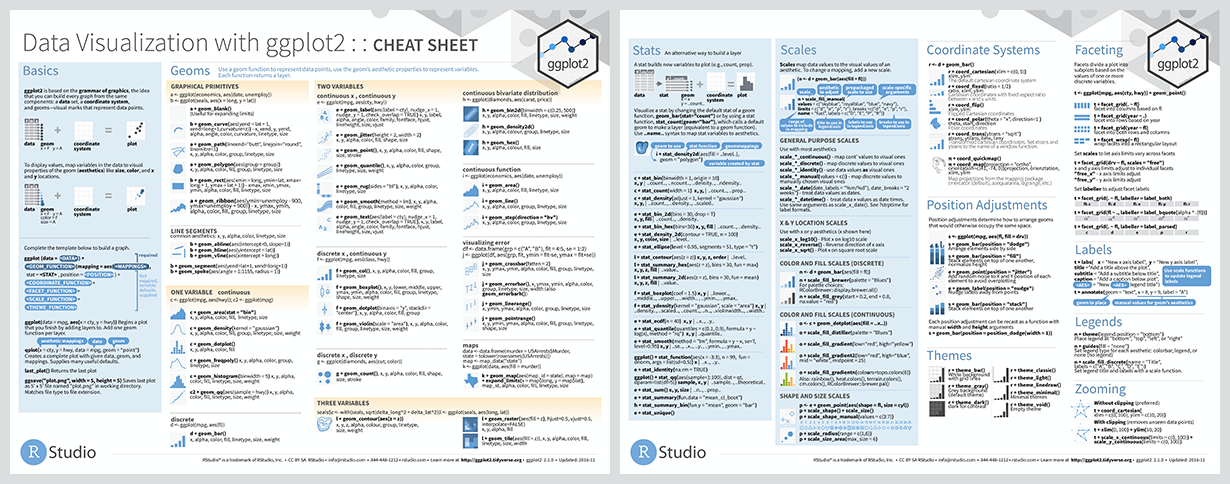
\includegraphics[width=17.08in]{atlas/ggplot_cheat_sheet} \end{center}

For example, you can plot a column chart by passing the \texttt{sa3\_income} dataset into \texttt{ggplot()} (``make a chart with this data''). This completes the first step -- data -- and produces an empty plot:

\begin{Shaded}
\begin{Highlighting}[]
\NormalTok{professionals }\OperatorTok\StringTok{ }
\StringTok{        }\KeywordTok{ggplot}\NormalTok{()}
\end{Highlighting}
\end{Shaded}


\includegraphics{Data_visualisation_files/figure-latex/empty_plot-1.pdf}

Next, set the \texttt{aes} (aesthetics) to \texttt{x\ =\ state} (``make the x-axis represent state''), \texttt{y\ =\ pop} (``the y-axis should represent population''), and \texttt{fill\ =\ year} (``the fill colour represents year''). Now \texttt{ggplot} knows where things should \emph{go}.

If we just plot that, you'll see that \texttt{ggplot} knows a little bit more about what we're trying to do. It has the states on the x-axis and range of populations on the y-axis:

\begin{Shaded}
\begin{Highlighting}[]
\NormalTok{professionals }\OperatorTok\StringTok{ }
\StringTok{        }\KeywordTok{ggplot}\NormalTok{(}\KeywordTok{aes}\NormalTok{(}\DataTypeTok{x =}\NormalTok{ workers,}
                   \DataTypeTok{y =}\NormalTok{ median_income,}
                   \DataTypeTok{colour =}\NormalTok{ gender))}
\end{Highlighting}
\end{Shaded}

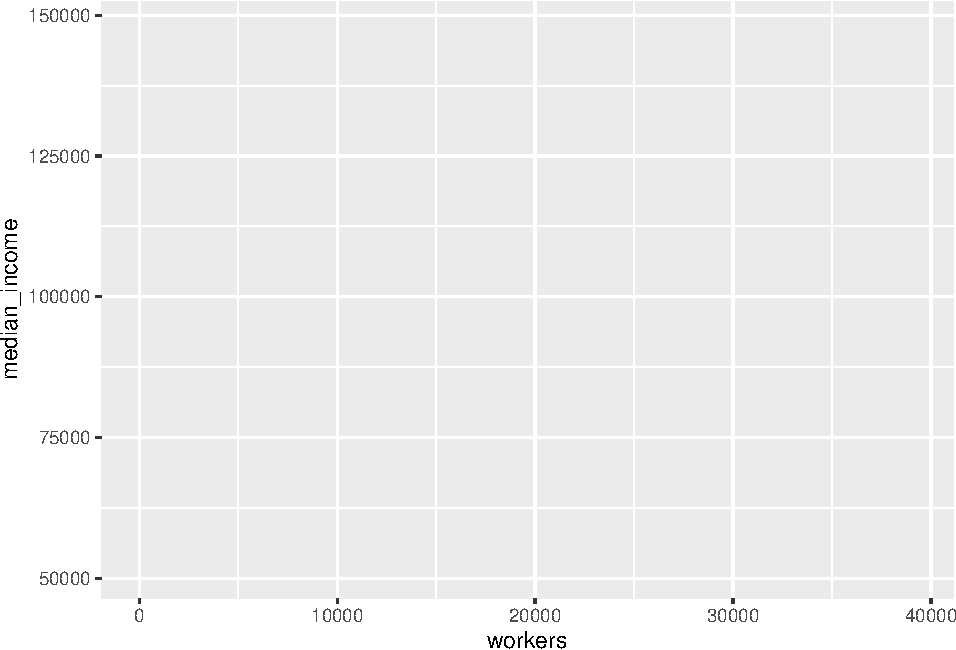
\includegraphics{Data_visualisation_files/figure-latex/empty_aes-1.pdf}

Now that \texttt{ggplot} knows where things should go, it needs to how to \emph{plot} them on the chart. For this we use \texttt{geoms}. Tell \texttt{ggplot} to take the things it knows and plot them as a column chart by using \texttt{geom\_col}:

\begin{Shaded}
\begin{Highlighting}[]
\NormalTok{professionals }\OperatorTok
\StringTok{        }\KeywordTok{ggplot}\NormalTok{(}\KeywordTok{aes}\NormalTok{(}\DataTypeTok{x =}\NormalTok{ workers,}
                   \DataTypeTok{y =}\NormalTok{ median_income,}
                   \DataTypeTok{colour =}\NormalTok{ gender)) }\OperatorTok{+}\StringTok{ }
\StringTok{        }\KeywordTok{geom_point}\NormalTok{()}
\end{Highlighting}
\end{Shaded}

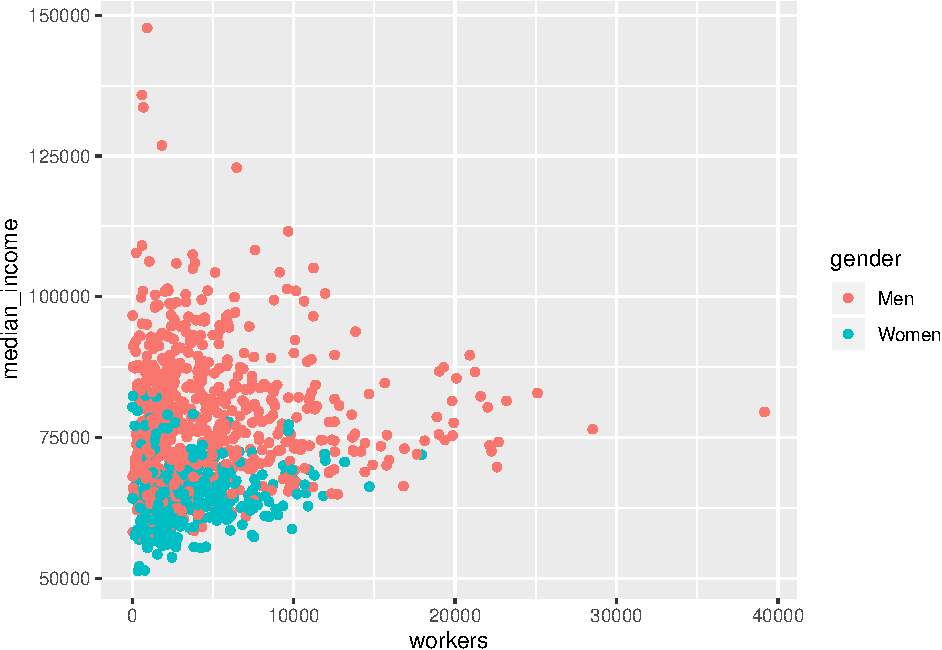
\includegraphics{Data_visualisation_files/figure-latex/complete_plot-1.pdf}

Great! There are a couple of quick things we can do to make the chart a bit clearer. There are points for each group in each year, which we probably don't need. So filter the data before you pass it to \texttt{ggplot} to just include 2015: \texttt{filter(year\ ==\ 2015)}. There will still be lots of overlapping points, so set the opacity to below one with \texttt{alpha\ =\ 0.5}. The \texttt{workers} x-axis can be changed to a log scale with \texttt{scale\_x\_log10}.

\begin{Shaded}
\begin{Highlighting}[]
\NormalTok{professionals }\OperatorTok\StringTok{ }
\StringTok{        }\KeywordTok{ggplot}\NormalTok{(}\KeywordTok{aes}\NormalTok{(}\DataTypeTok{x =}\NormalTok{ workers,}
                   \DataTypeTok{y =}\NormalTok{ median_income,}
                   \DataTypeTok{colour =}\NormalTok{ gender)) }\OperatorTok{+}\StringTok{ }
\StringTok{        }\KeywordTok{geom_point}\NormalTok{(}\DataTypeTok{alpha =} \FloatTok{.5}\NormalTok{) }\OperatorTok{+}\StringTok{ }
\StringTok{        }\KeywordTok{scale_x_log10}\NormalTok{()}
\end{Highlighting}
\end{Shaded}

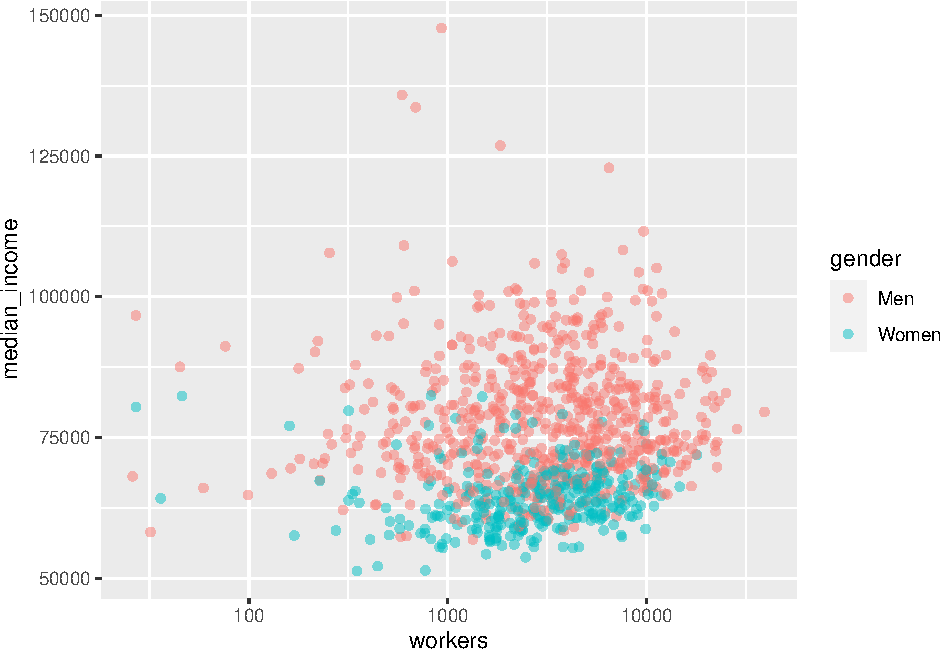
\includegraphics{Data_visualisation_files/figure-latex/with_changes-1.pdf}

That looks a bit better. The following sections in this chapter will cover a broad range of charts and designs, but they will all use the same building-blocks of \texttt{data}, \texttt{aes}, and \texttt{geom}.

The rest of the chapter will explore:

\begin{itemize}
\tightlist
\item
  Exploratory data visualisation
\item
  Grattanising your charts and choosing colours
\item
  Saving charts according to Grattan templates
\item
  Making bar, line, scatter and distribution plots
\item
  Making maps and interactive charts
\item
  Adding chart labels
\end{itemize}

\hypertarget{exploratory-data-visualisation}{%
\section{Exploratory data visualisation}\label{exploratory-data-visualisation}}

Plotting your data early in the analysis stage can help you quickly identify outliers, oddities, things that don't look quite right.

\hypertarget{making-grattan-y-charts}{%
\section{Making Grattan-y charts}\label{making-grattan-y-charts}}

The \texttt{grattantheme} package contains functions that help \emph{Grattanise} your charts. It is hosted here: \url{https://github.com/mattcowgill/grattantheme}

You can install it with \texttt{remotes::install\_github} from the package:

\begin{Shaded}
\begin{Highlighting}[]
\KeywordTok{install.packages}\NormalTok{(}\StringTok{"remotes"}\NormalTok{)}
\NormalTok{remotes}\OperatorTok{::}\KeywordTok{install_github}\NormalTok{(}\StringTok{"mattcowgill/grattantheme"}\NormalTok{)}
\end{Highlighting}
\end{Shaded}

The key functions of \texttt{grattantheme} are:

\begin{itemize}
\tightlist
\item
  \texttt{theme\_grattan}: set size, font and colour defaults that adhere to the Grattan style guide.
\item
  \texttt{grattan\_y\_continuous}: sets the right defaults for a continuous y-axis.
\item
  \texttt{grattan\_colour\_continuous}: pulls colours from the Grattan colour palette for \texttt{colour} aesthetics.
\item
  \texttt{grattan\_fill\_continuous}: pulls colours from the Grattan colour palette for \texttt{fill} aesthetics.
\item
  \texttt{grattan\_save}: a save function that exports charts in correct report or presentation dimensions.
\end{itemize}

This section will run through some examples of \emph{Grattanising} charts. The \texttt{ggplot} functions are explored in more detail in the next section.

\hypertarget{making-grattan-charts}{%
\subsection{Making Grattan charts}\label{making-grattan-charts}}

Start with a scatterplot, similar to the one made above:

\begin{Shaded}
\begin{Highlighting}[]
\NormalTok{base_chart <-}\StringTok{ }\NormalTok{professionals }\OperatorTok\StringTok{ }
\StringTok{        }\KeywordTok{ggplot}\NormalTok{(}\KeywordTok{aes}\NormalTok{(}\DataTypeTok{x =}\NormalTok{ workers,}
                   \DataTypeTok{y =}\NormalTok{ median_income,}
                   \DataTypeTok{colour =}\NormalTok{ gender)) }\OperatorTok{+}\StringTok{ }
\StringTok{        }\KeywordTok{geom_point}\NormalTok{(}\DataTypeTok{alpha =} \FloatTok{.5}\NormalTok{) }\OperatorTok{+}\StringTok{ }
\StringTok{        }\KeywordTok{labs}\NormalTok{(}\DataTypeTok{title =} \StringTok{"More professionals, the more they earn"}\NormalTok{,}
             \DataTypeTok{subtitle =} \StringTok{"Median income of professional workers in SA3s"}\NormalTok{,}
             \DataTypeTok{x =} \StringTok{"Number of professional workers"}\NormalTok{,}
             \DataTypeTok{y =} \StringTok{"Median income"}\NormalTok{,}
             \DataTypeTok{caption =} \StringTok{"Source: ABS Estimates of Personal Income for Small Areas, 2011-2016"}\NormalTok{)}

\NormalTok{base_chart}
\end{Highlighting}
\end{Shaded}

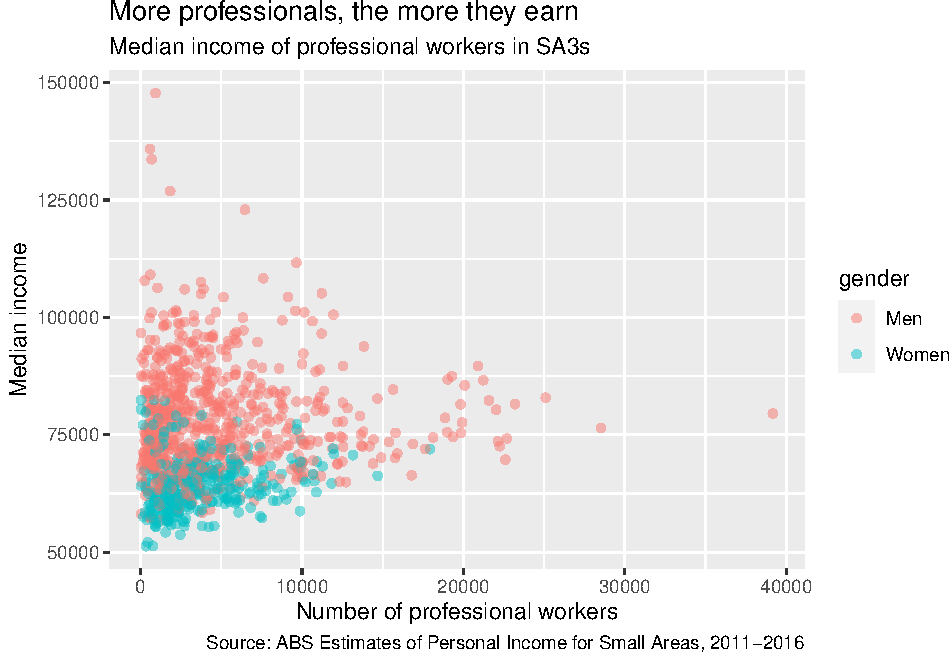
\includegraphics{Data_visualisation_files/figure-latex/base_chart-1.pdf}

Let's make it Grattany. First, add \texttt{theme\_grattan} to your plot:

\begin{Shaded}
\begin{Highlighting}[]
\NormalTok{base_chart }\OperatorTok{+}
\StringTok{        }\KeywordTok{theme_grattan}\NormalTok{(}\DataTypeTok{chart_type =} \StringTok{"scatter"}\NormalTok{)}
\end{Highlighting}
\end{Shaded}

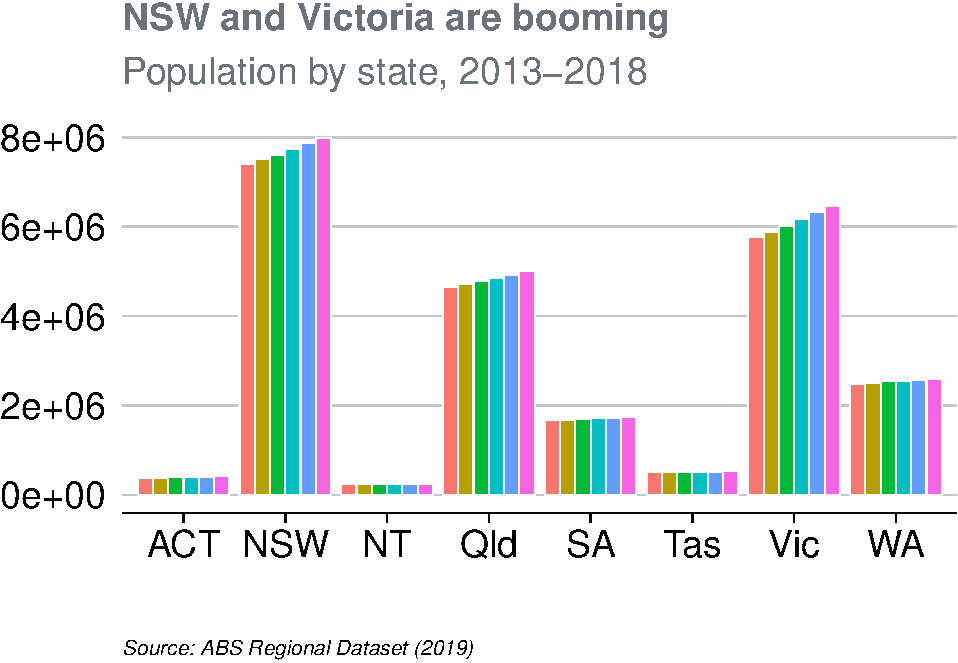
\includegraphics{Data_visualisation_files/figure-latex/add_theme_grattan-1.pdf}

Then use \texttt{grattan\_y\_continuous} to adjust the y-axis. This takes the same arguments as the standard \texttt{scale\_y\_continuous} function, but has Grattan defaults built in. Use it to set the labels as dollars (with \texttt{scales::dollar()}) and to give the y-axis some breathing room (starting at \$50,000 rather than the minimum point).
Also add \texttt{scale\_x\_log10} to make the x-axis a log10 scale, telling it to format the labels as numbers with commas (using \texttt{scales::comma()}).\footnote{The \texttt{dollar} and \texttt{comma} commands are functions, but can be used without \texttt{()}. Using \texttt{dollar()} or \texttt{comma()} works too, and you can provide arguments that adjust their output: eg \texttt{dollar(suffix\ =\ "million")}}

\begin{Shaded}
\begin{Highlighting}[]
\NormalTok{base_chart }\OperatorTok{+}
\StringTok{        }\KeywordTok{theme_grattan}\NormalTok{(}\DataTypeTok{chart_type =} \StringTok{"scatter"}\NormalTok{) }\OperatorTok{+}
\StringTok{        }\KeywordTok{grattan_y_continuous}\NormalTok{(}\DataTypeTok{labels =}\NormalTok{ dollar, }\DataTypeTok{limits =} \KeywordTok{c}\NormalTok{(}\FloatTok{50e3}\NormalTok{, }\OtherTok{NA}\NormalTok{)) }\OperatorTok{+}
\StringTok{        }\KeywordTok{scale_x_log10}\NormalTok{(}\DataTypeTok{labels =}\NormalTok{ comma) }
\end{Highlighting}
\end{Shaded}

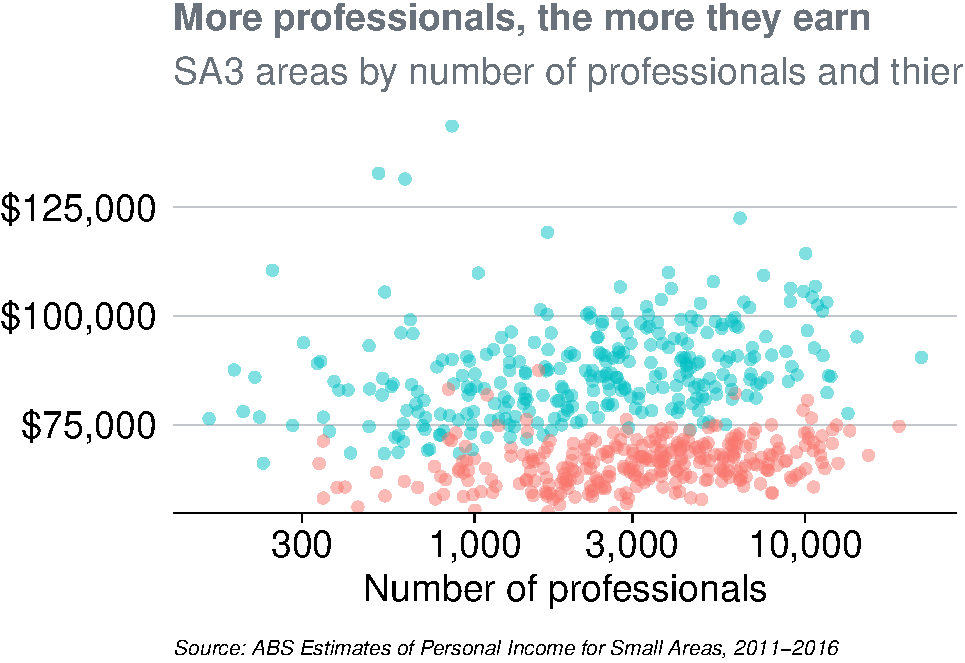
\includegraphics{Data_visualisation_files/figure-latex/add_grattan_y_continuous-1.pdf}

To define \texttt{colour} colours, use \texttt{grattan\_colour\_manual} with the number of colours you need (two, in this case):

\begin{Shaded}
\begin{Highlighting}[]
\NormalTok{prof_chart <-}\StringTok{ }\NormalTok{base_chart }\OperatorTok{+}
\StringTok{        }\KeywordTok{theme_grattan}\NormalTok{(}\DataTypeTok{chart_type =} \StringTok{"scatter"}\NormalTok{) }\OperatorTok{+}
\StringTok{        }\KeywordTok{grattan_y_continuous}\NormalTok{(}\DataTypeTok{labels =}\NormalTok{ dollar, }\DataTypeTok{limits =} \KeywordTok{c}\NormalTok{(}\FloatTok{50e3}\NormalTok{, }\OtherTok{NA}\NormalTok{)) }\OperatorTok{+}
\StringTok{        }\KeywordTok{scale_x_log10}\NormalTok{(}\DataTypeTok{labels =}\NormalTok{ comma) }\OperatorTok{+}
\StringTok{        }\KeywordTok{grattan_colour_manual}\NormalTok{(}\DecValTok{2}\NormalTok{) }

\NormalTok{prof_chart}
\end{Highlighting}
\end{Shaded}

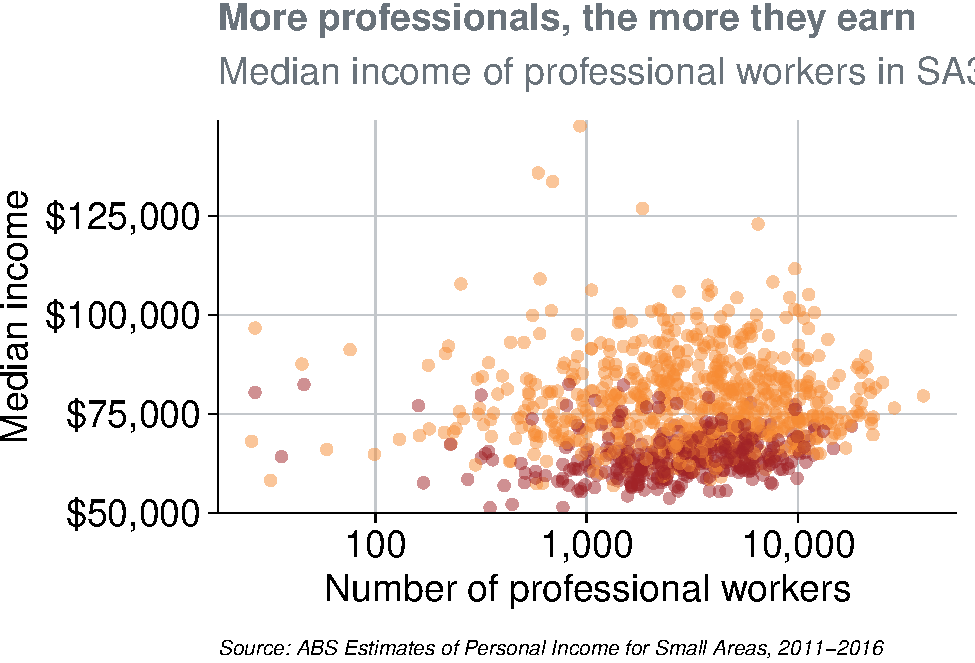
\includegraphics{Data_visualisation_files/figure-latex/add_fill-1.pdf}

Nice chart! Now you can save it and share it with the world.

\hypertarget{saving-grattan-charts}{%
\subsection{Saving Grattan charts}\label{saving-grattan-charts}}

The \texttt{grattan\_save} function saves your charts according to Grattan templates. It takes these arguments:

\begin{itemize}
\tightlist
\item
  \texttt{filename}: the path, name and file-type of your saved chart. eg: \texttt{"atlas/professionals\_chart.pdf"}.
\item
  \texttt{object}: the R object that you want to save. eg: \texttt{prof\_chart}. If left blank, it grabs the last chart that was displayed.
\item
  \texttt{type}: the Grattan template to be used. This is one of:

  \begin{itemize}
  \tightlist
  \item
    \texttt{"normal"} The default. Use for normal Grattan report charts, or to paste into a 4:3 PowerPoint slide. Width: 22.2cm, height: 14.5cm.
  \item
    \texttt{"normal\_169"} Only useful for pasting into a 16:9 format Grattan PowerPoint slide. Width: 30cm, height: 14.5cm.
  \item
    \texttt{"tiny"} Fills the width of a column in a Grattan report, but is shorter than usual. Width: 22.2cm, height: 11.1cm.
  \item
    \texttt{"wholecolumn"} Takes up a whole column in a Grattan report. Width: 22.2cm, height: 22.2cm.
  \item
    \texttt{"fullpage"} Fills a whole page of a Grattan report. Width: 44.3cm, height: 22.2cm.
  \item
    \texttt{"fullslide"} Creates an image that looks like a 4:3 Grattan PowerPoint slide, complete with logo. Width: 25.4cm, height: 19.0cm.
  \item
    \texttt{"fullslide\_169"} Creates` an image that looks like a 16:9 Grattan PowerPoint slide, complete with logo. Use this to drop into standard presentations. Width: 33.9cm, height: 19.0cm
  \item
    \texttt{"blog"} Creates a 4:3 image that looks like a Grattan PowerPoint slide, but with less border whitespace than `fullslide'."
  \item
    \texttt{"fullslide\_44"\ Creates} an image that looks like a 4:4 Grattan PowerPoint slide. This may be useful for taller charts for the Grattan blog; not useful for any other purpose. Width: 25.4cm, height: 25.4cm.
  \item
    Set \texttt{type\ =\ "all"} to save your chart in all available sizes.
  \end{itemize}
\item
  \texttt{height}: override the height set by \texttt{type}. This can be useful for really long charts in blogposts.
\item
  \texttt{save\_data}: exports a \texttt{csv} file containing the data used in the chart.
\item
  \texttt{force\_labs}: override the removal of labels for a particular \texttt{type}. eg \texttt{force\_labs\ =\ TRUE} will keep the y-axis label.
\end{itemize}

To save the \texttt{prof\_chart} plot created above as a whole-column chart for a \textbf{report}:

\begin{Shaded}
\begin{Highlighting}[]
\KeywordTok{grattan_save}\NormalTok{(}\StringTok{"atlas/professionals_chart_report.pdf"}\NormalTok{, prof_chart, }\DataTypeTok{type =} \StringTok{"wholecolumn"}\NormalTok{)}
\end{Highlighting}
\end{Shaded}

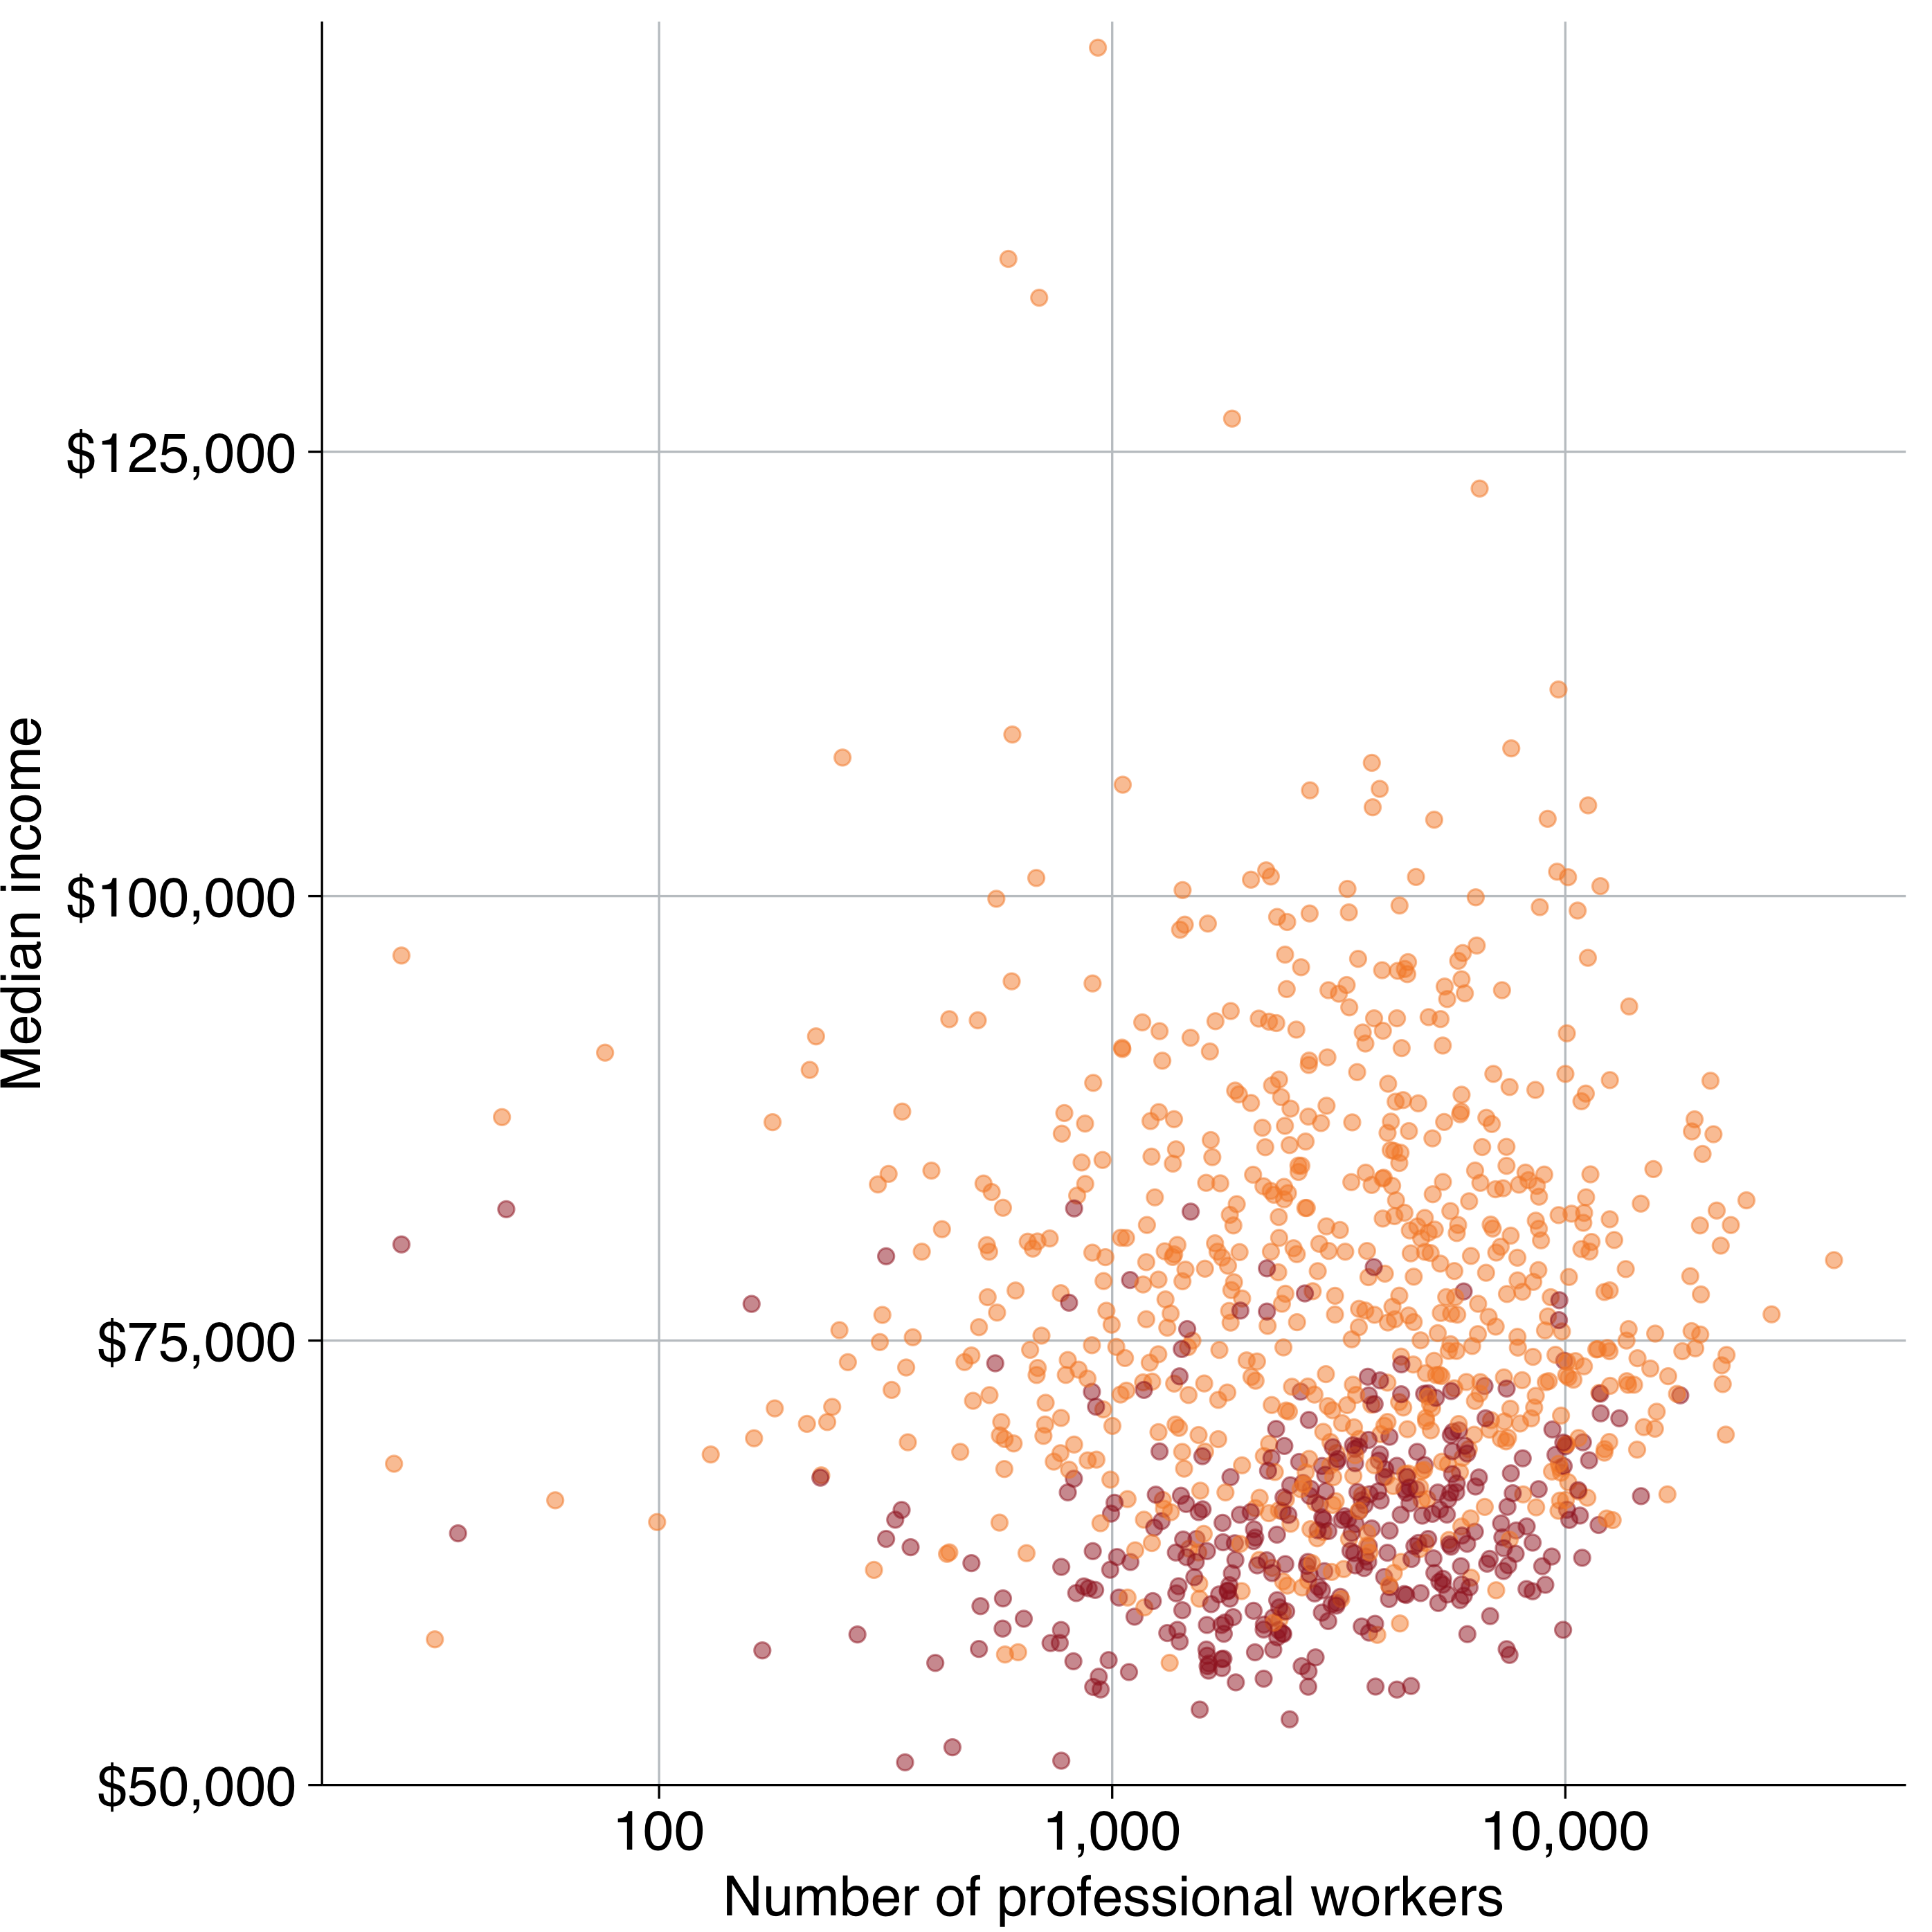
\includegraphics[width=38.76in]{atlas/professionals_chart_report}

To save it as a \textbf{presentation} slide instead, use \texttt{type\ =\ "fullslide"}:

\begin{Shaded}
\begin{Highlighting}[]
\KeywordTok{grattan_save}\NormalTok{(}\StringTok{"atlas/professionals_chart_presentation.pdf"}\NormalTok{, prof_chart, }\DataTypeTok{type =} \StringTok{"fullslide"}\NormalTok{)}
\end{Highlighting}
\end{Shaded}

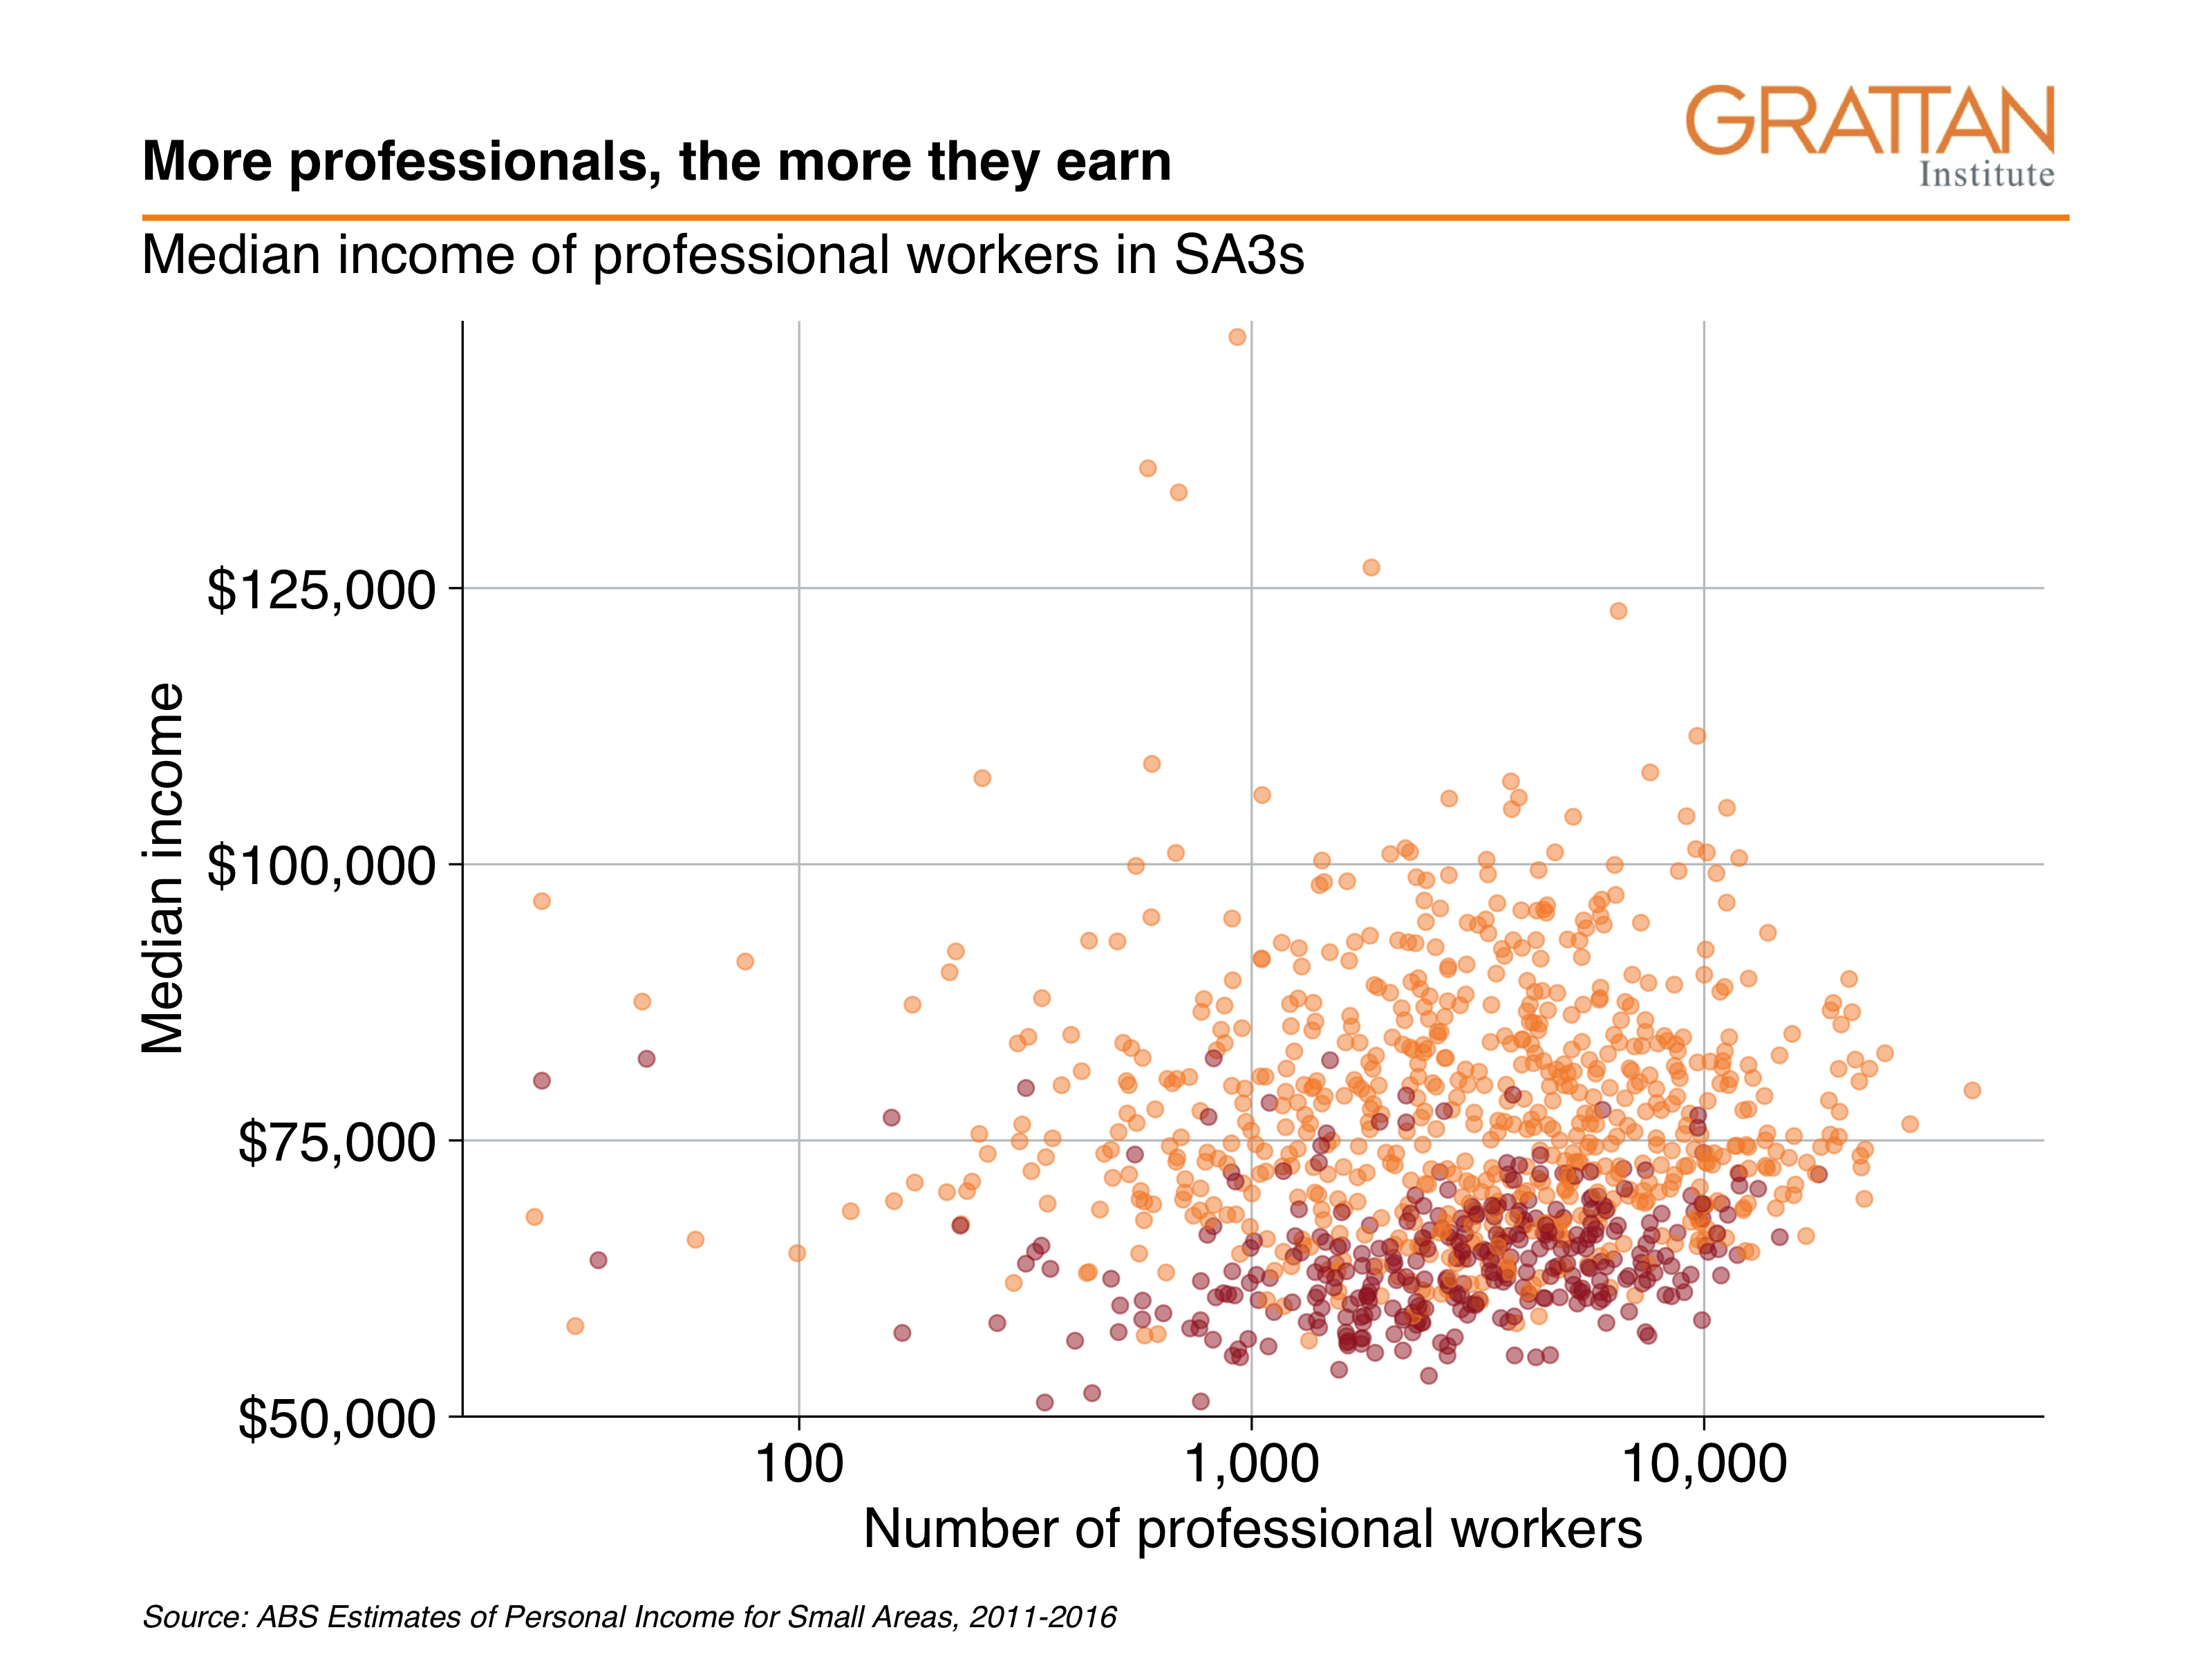
\includegraphics[width=44.44in]{atlas/professionals_chart_presentation}

Or, if you want to emphasise the point in a \emph{really tall} chart for a \textbf{blogpost}, you can use \texttt{type\ =\ "blog"} and adjust the \texttt{height} to be 50cm. Also note that because this is for the blog, you should save it as a \texttt{png} file:

\begin{Shaded}
\begin{Highlighting}[]
\KeywordTok{grattan_save}\NormalTok{(}\StringTok{"atlas/professionals_chart_blog.png"}\NormalTok{, prof_chart, }
             \DataTypeTok{type =} \StringTok{"blog"}\NormalTok{, }\DataTypeTok{height =} \DecValTok{30}\NormalTok{)}
\end{Highlighting}
\end{Shaded}

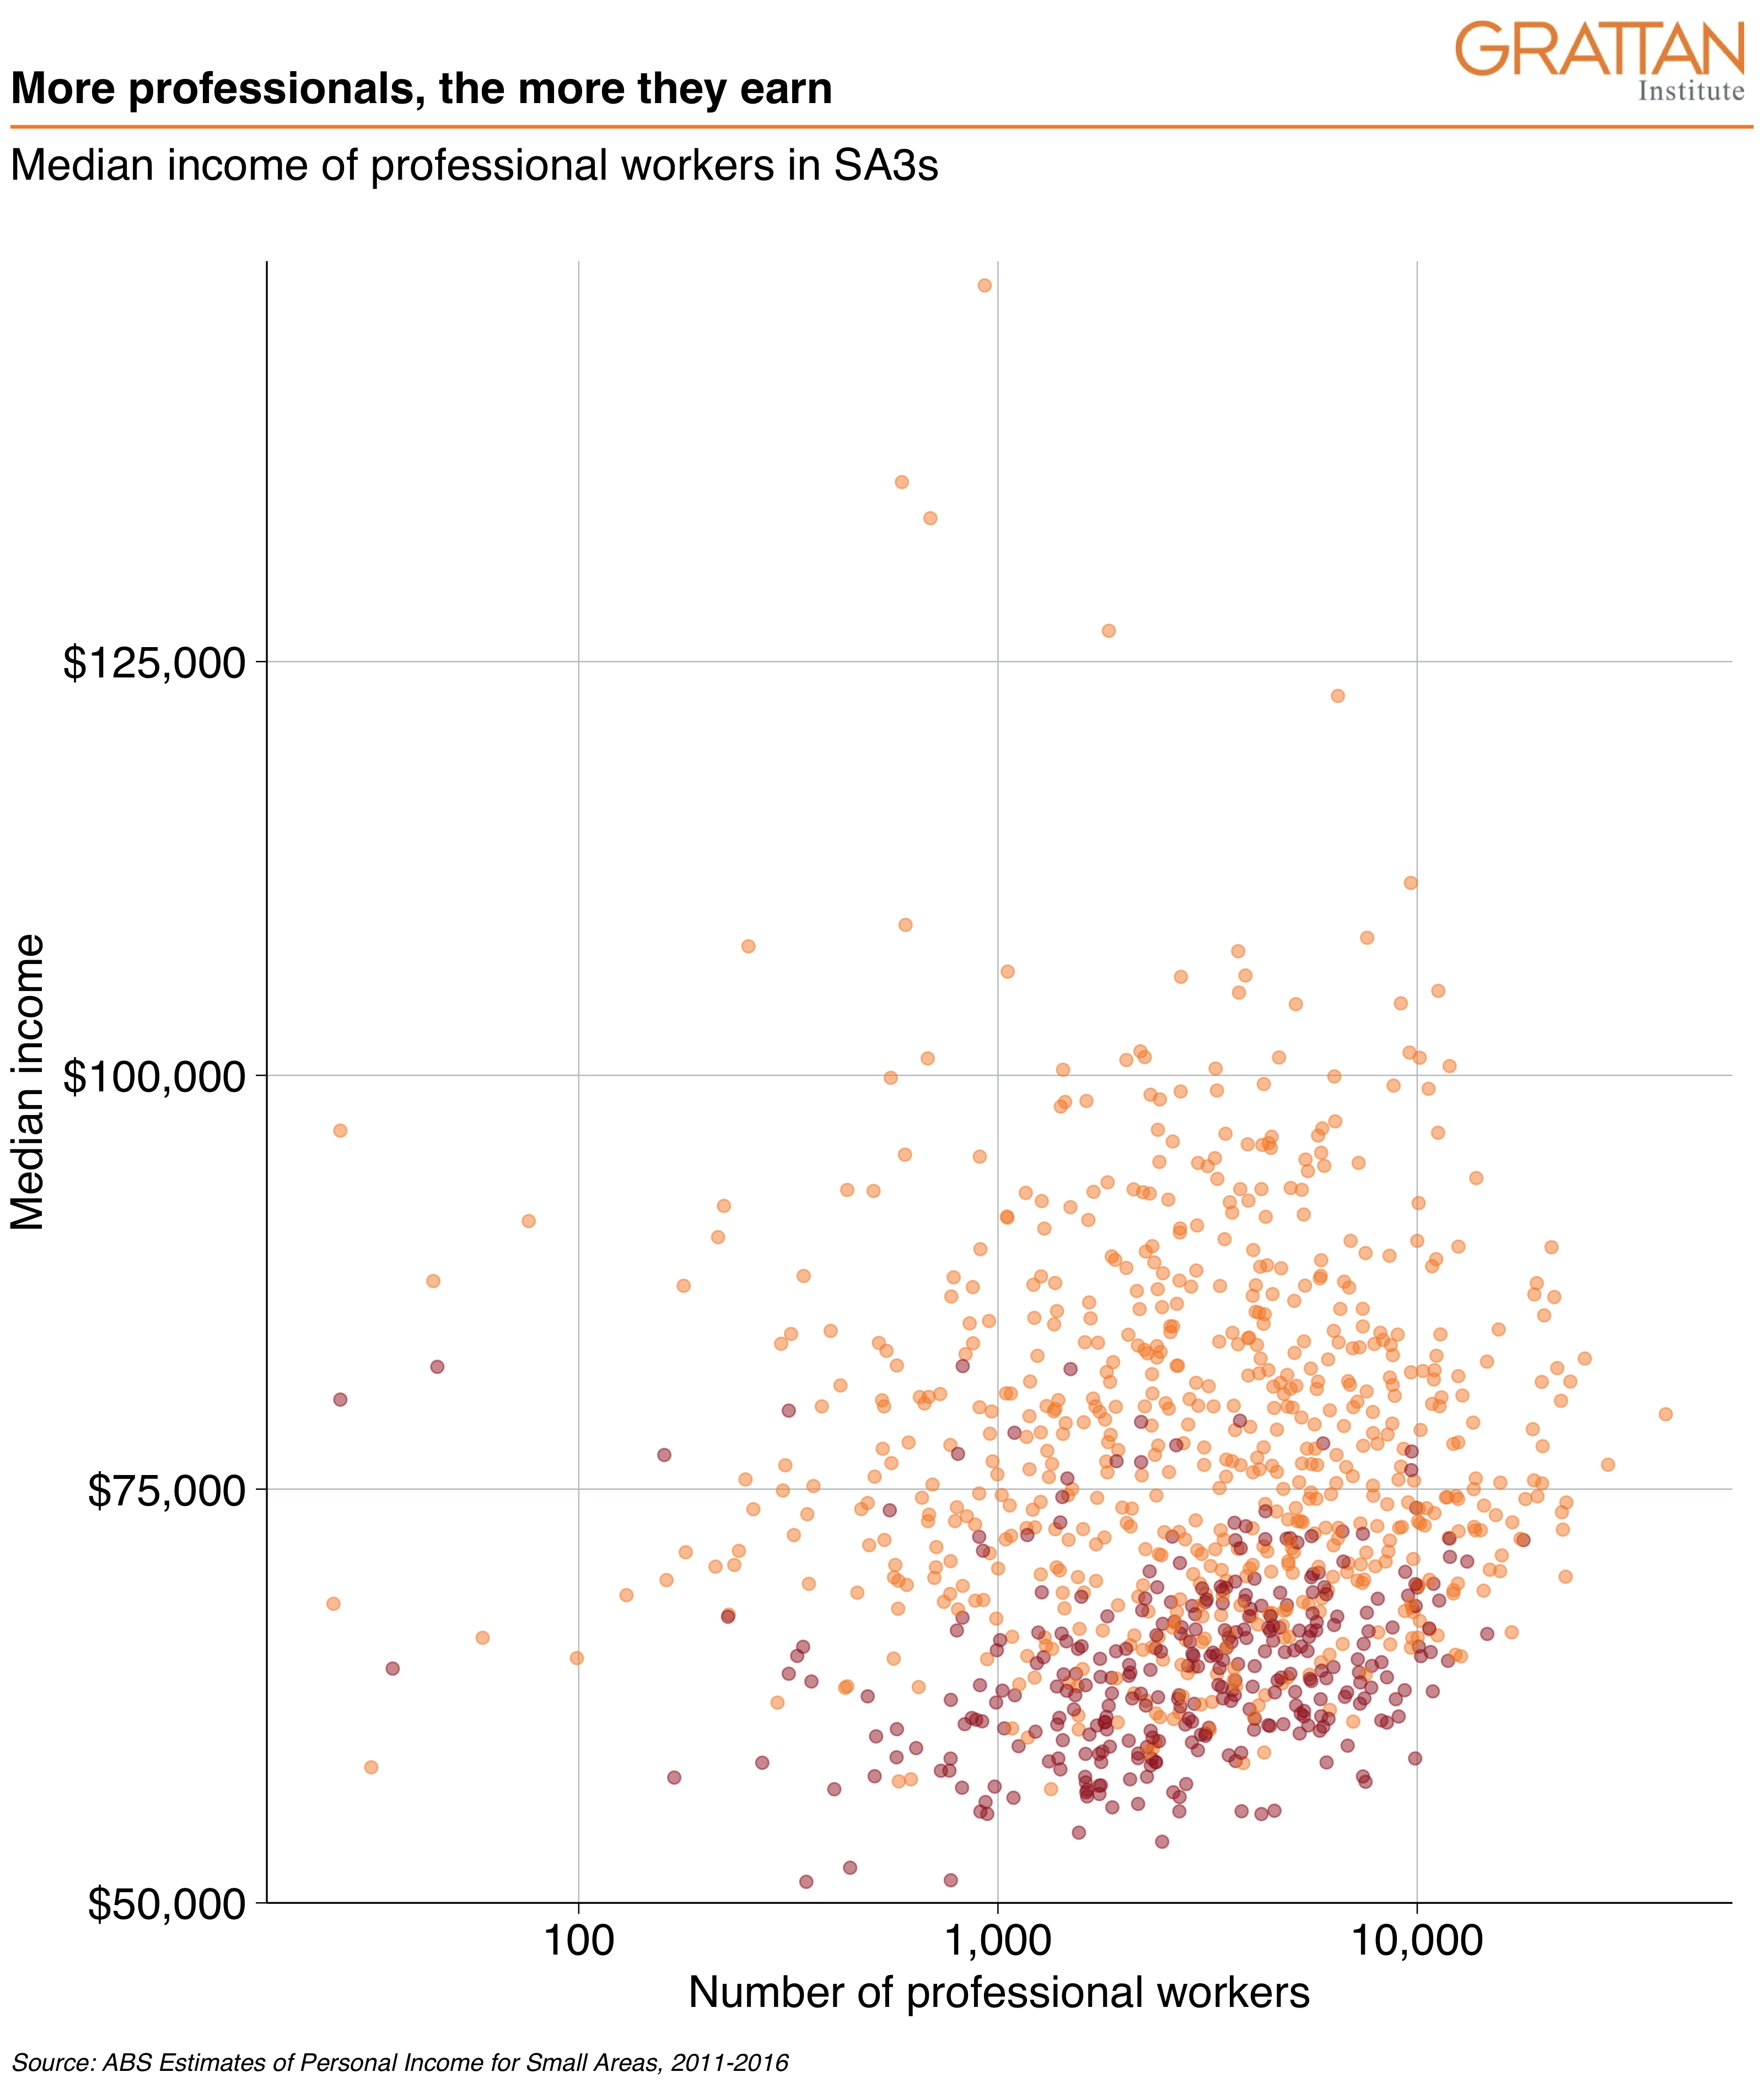
\includegraphics[width=44.44in]{atlas/professionals_chart_blog}

And that's it! The following sections will go into more detail about different chart types in R, but you'll mostly use the same basic \texttt{grattantheme} formatting you've used here.

\hypertarget{adding-labels}{%
\section{Adding labels}\label{adding-labels}}

Labels can be a bit finicky -- especially compared to labelling charts visually in PowerPoint. \ldots{}

Labels can be done in two broad ways:

\begin{enumerate}
\def\labelenumi{\arabic{enumi}.}
\tightlist
\item
  Labelling every single data point on your chart. Grattan charts rarely do this.
\item
  Labelling some of the data points on your chart. This is how you label Grattan charts: label on item in a group and let the reader join the dots.
\end{enumerate}

We'll look at the first approach so you can get a feel for how the labelling geoms -- \texttt{geom\_label} and \texttt{geom\_text} (and some useful extensions) -- work. It won't be pretty.

\begin{Shaded}
\begin{Highlighting}[]
\NormalTok{prof_chart }\OperatorTok{+}
\StringTok{  }\KeywordTok{geom_text}\NormalTok{(}\KeywordTok{aes}\NormalTok{(}\DataTypeTok{label =}\NormalTok{ gender))}
\end{Highlighting}
\end{Shaded}

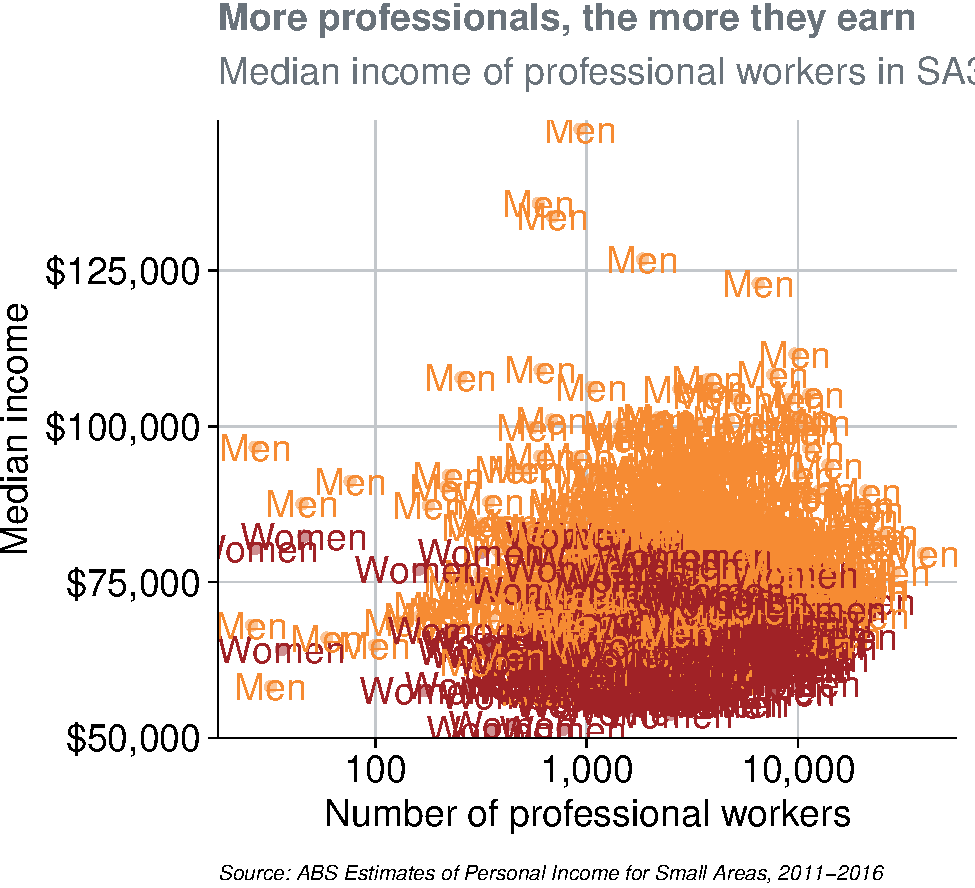
\includegraphics{Data_visualisation_files/figure-latex/add_annotate-1.pdf}

Great! That looks \emph{terrible}. \texttt{geom\_text} is labelling each individual point because it has been told to do so. Just like \texttt{geom\_point}, it takes the \texttt{x} and \texttt{y} aesthetics of each observation, then plots the \texttt{label} at that location. But we just want to label one of the points for \texttt{female} and one for \texttt{male}.

To do this, we can create a new dataset that just contains one observation each. Here, you're filtering the dataset to include \emph{only} the female/male observations that have the most people:

\begin{Shaded}
\begin{Highlighting}[]
\NormalTok{label_data <-}\StringTok{ }\NormalTok{professionals }\OperatorTok\StringTok{ }
\StringTok{  }\KeywordTok{group_by}\NormalTok{(gender) }\OperatorTok\StringTok{ }
\StringTok{  }\KeywordTok{filter}\NormalTok{(workers }\OperatorTok{==}\StringTok{ }\KeywordTok{max}\NormalTok{(workers)) }\OperatorTok\StringTok{ }
\StringTok{  }\KeywordTok{ungroup}\NormalTok{()}

\NormalTok{label_data}
\end{Highlighting}
\end{Shaded}

\begin{verbatim}
## # A tibble: 2 x 14
##     sa3 sa3_name sa3_sqkm sa3_income_perc~ state occupation occ_short prof 
##   <dbl> <chr>       <dbl>            <dbl> <chr> <chr>      <chr>     <chr>
## 1 11703 Sydney ~     25.1               84 NSW   Professio~ Professi~ Prof~
## 2 11703 Sydney ~     25.1               84 NSW   Professio~ Professi~ Prof~
## # ... with 6 more variables: gender <chr>, year <dbl>,
## #   median_income <dbl>, average_income <dbl>, total_income <dbl>,
## #   workers <dbl>
\end{verbatim}

And then tell \texttt{geom\_text} to look at \emph{that} dataset:

\begin{Shaded}
\begin{Highlighting}[]
\NormalTok{prof_chart }\OperatorTok{+}
\StringTok{  }\KeywordTok{geom_text}\NormalTok{(}\DataTypeTok{data =}\NormalTok{ label_data,}
            \KeywordTok{aes}\NormalTok{(}\DataTypeTok{label =}\NormalTok{ gender))}
\end{Highlighting}
\end{Shaded}

\includegraphics{Data_visualisation_files/figure-latex/unnamed-chunk-2-1.pdf}

Okay, not bad. The labels go off the chart. You could fix this by shortening the labels either inside the \texttt{label\_data}:

\begin{Shaded}
\begin{Highlighting}[]
\NormalTok{label_data_short <-}\StringTok{ }\NormalTok{label_data }\OperatorTok\StringTok{ }
\StringTok{  }\KeywordTok{mutate}\NormalTok{(}\DataTypeTok{gender_label =} \KeywordTok{if_else}\NormalTok{(gender }\OperatorTok{==}\StringTok{ "Females"}\NormalTok{, }
                             \StringTok{"Women"}\NormalTok{, }
                             \StringTok{"Men"}\NormalTok{))}

\NormalTok{prof_chart }\OperatorTok{+}
\StringTok{  }\KeywordTok{geom_text}\NormalTok{(}\DataTypeTok{data =}\NormalTok{ label_data_short,}
            \KeywordTok{aes}\NormalTok{(}\DataTypeTok{label =}\NormalTok{ gender_label))}
\end{Highlighting}
\end{Shaded}

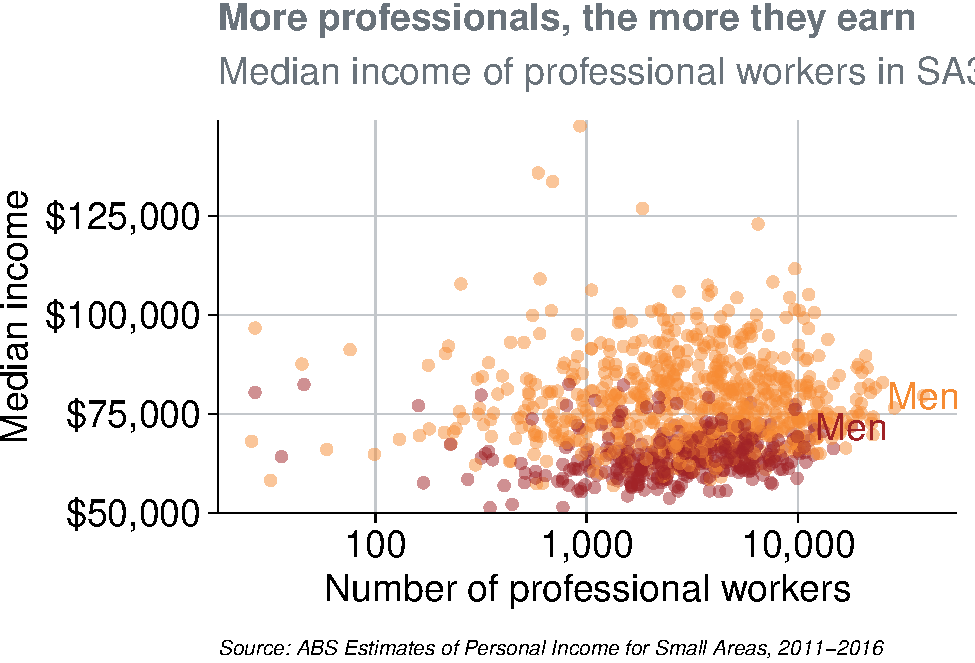
\includegraphics{Data_visualisation_files/figure-latex/unnamed-chunk-3-1.pdf}

\emph{Or} you could adjust the label values directly inside the aesthetics call. Note that this means you have to provide a vector that is the same length as the number of observations in the data (a length of two, in this case).

\begin{Shaded}
\begin{Highlighting}[]
\NormalTok{prof_chart }\OperatorTok{+}
\StringTok{  }\KeywordTok{geom_text}\NormalTok{(}\DataTypeTok{data =}\NormalTok{ label_data,}
            \KeywordTok{aes}\NormalTok{(}\DataTypeTok{label =} \KeywordTok{c}\NormalTok{(}\StringTok{"Female"}\NormalTok{, }\StringTok{"Male"}\NormalTok{)))}
\end{Highlighting}
\end{Shaded}

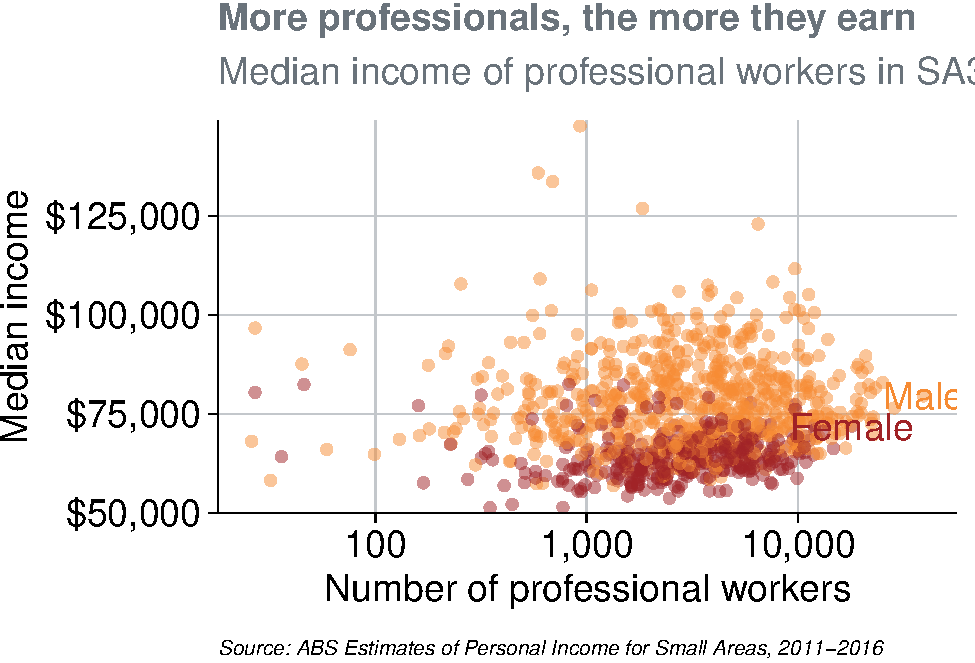
\includegraphics{Data_visualisation_files/figure-latex/unnamed-chunk-4-1.pdf}

To have more freedom over \emph{where} your labels are placed, you can create a dataset yourself. Add the \texttt{x} and \texttt{y} values for your labels, and the label names.\footnote{We are using the \texttt{tribble} function here to make it a little bit clearer what values apply to which gender. The `normal' way to create a tibble is with the \texttt{tibble} function: \texttt{tibble(x\ =\ c(10,\ 100),\ y\ =\ c(100,\ 10))}, etc.}

\begin{Shaded}
\begin{Highlighting}[]
\NormalTok{self_label <-}\StringTok{ }\KeywordTok{tribble}\NormalTok{(}
  \OperatorTok{~}\NormalTok{gender, }\OperatorTok{~}\NormalTok{workers,   }\OperatorTok{~}\NormalTok{median_income,}
  \StringTok{"Women"}\NormalTok{,    }\DecValTok{23000}\NormalTok{,            }\DecValTok{55000}\NormalTok{,}
  \StringTok{"Men"}\NormalTok{,      }\DecValTok{23000}\NormalTok{,           }\DecValTok{110000}\NormalTok{)}


\NormalTok{self_label}
\end{Highlighting}
\end{Shaded}

\begin{verbatim}
## # A tibble: 2 x 3
##   gender workers median_income
##   <chr>    <dbl>         <dbl>
## 1 Women    23000         55000
## 2 Men      23000        110000
\end{verbatim}

\begin{Shaded}
\begin{Highlighting}[]
\NormalTok{prof_chart }\OperatorTok{+}
\StringTok{  }\KeywordTok{geom_text}\NormalTok{(}\DataTypeTok{data =}\NormalTok{ self_label,}
            \KeywordTok{aes}\NormalTok{(}\DataTypeTok{label =}\NormalTok{ gender), }
            \DataTypeTok{hjust =} \DecValTok{1}\NormalTok{)}
\end{Highlighting}
\end{Shaded}

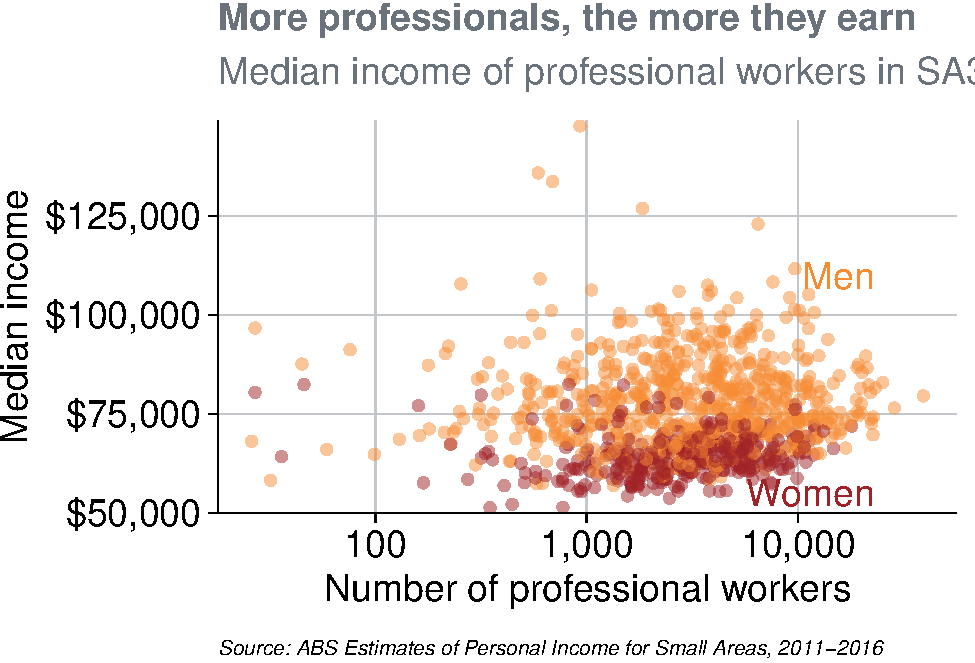
\includegraphics{Data_visualisation_files/figure-latex/unnamed-chunk-6-1.pdf}

{[}cover \texttt{annotate}{]}

\hypertarget{chart-cookbook}{%
\chapter{Chart cookbook}\label{chart-cookbook}}

This section takes you through a few often-used chart types.

\hypertarget{set-up}{%
\section{Set up}\label{set-up}}

\begin{Shaded}
\begin{Highlighting}[]
\KeywordTok{library}\NormalTok{(tidyverse)}
\KeywordTok{library}\NormalTok{(grattantheme)}
\KeywordTok{library}\NormalTok{(ggrepel)}
\KeywordTok{library}\NormalTok{(absmapsdata)}
\KeywordTok{library}\NormalTok{(sf)}
\KeywordTok{library}\NormalTok{(scales)}
\KeywordTok{library}\NormalTok{(janitor)}
\CommentTok{# this might be hairy; should get `grattools` happening:}
\KeywordTok{library}\NormalTok{(grattan)}
\end{Highlighting}
\end{Shaded}

\begin{Shaded}
\begin{Highlighting}[]
\CommentTok{# note: to be added to grattantheme; remove this when done}
\NormalTok{grattan_label_repel <-}\StringTok{ }\ControlFlowTok{function}\NormalTok{(..., }\DataTypeTok{size =} \DecValTok{18}\NormalTok{) \{}

\NormalTok{  .size =}\StringTok{ }\NormalTok{size }\OperatorTok{/}\StringTok{ }\NormalTok{ggplot2}\OperatorTok{::}\NormalTok{.pt}
  
  \KeywordTok{geom_label_repel}\NormalTok{(..., }
                   \DataTypeTok{fill =} \StringTok{"white"}\NormalTok{,}
                   \DataTypeTok{label.padding =} \KeywordTok{unit}\NormalTok{(}\FloatTok{0.1}\NormalTok{, }\StringTok{"lines"}\NormalTok{), }
                   \DataTypeTok{label.size =} \DecValTok{0}\NormalTok{,}
                   \DataTypeTok{size =}\NormalTok{ .size)}
\NormalTok{\}}


\NormalTok{grattan_label <-}\StringTok{ }\ControlFlowTok{function}\NormalTok{(..., }\DataTypeTok{size =} \DecValTok{18}\NormalTok{) \{}

\NormalTok{  .size =}\StringTok{ }\NormalTok{size }\OperatorTok{/}\StringTok{ }\NormalTok{ggplot2}\OperatorTok{::}\NormalTok{.pt}
  
  \KeywordTok{geom_label}\NormalTok{(..., }
                   \DataTypeTok{fill =} \StringTok{"white"}\NormalTok{,}
                   \DataTypeTok{label.padding =} \KeywordTok{unit}\NormalTok{(}\FloatTok{0.1}\NormalTok{, }\StringTok{"lines"}\NormalTok{), }
                   \DataTypeTok{label.size =} \DecValTok{0}\NormalTok{,}
                   \DataTypeTok{size =}\NormalTok{ .size)}
\NormalTok{\}}
\end{Highlighting}
\end{Shaded}

The \texttt{sa3\_income} dataset will be used for all key examples in this chapter.\footnote{From \href{https://www.abs.gov.au/AUSSTATS/abs@.nsf/DetailsPage/6524.0.55.0022011-2016?OpenDocument}{ABS Employee income by occupation and sex, 2010-11 to 2016-16}} It is a long dataset from the ABS that contains the median income and number of workers by Statistical Area 3, occupation and sex between 2010 and 2016.

\begin{Shaded}
\begin{Highlighting}[]
\NormalTok{sa3_income <-}\StringTok{ }\KeywordTok{read_csv}\NormalTok{(}\StringTok{"data/sa3_income.csv"}\NormalTok{) }\OperatorTok\StringTok{ }
\StringTok{  }\KeywordTok{filter}\NormalTok{(}\OperatorTok{!}\KeywordTok{is.na}\NormalTok{(median_income),}
         \OperatorTok{!}\KeywordTok{is.na}\NormalTok{(average_income))}
\end{Highlighting}
\end{Shaded}

\begin{verbatim}
## Parsed with column specification:
## cols(
##   sa3 = col_double(),
##   sa3_name = col_character(),
##   sa3_sqkm = col_double(),
##   sa3_income_percentile = col_double(),
##   sa4_name = col_character(),
##   gcc_name = col_character(),
##   state = col_character(),
##   occupation = col_character(),
##   occ_short = col_character(),
##   prof = col_character(),
##   gender = col_character(),
##   year = col_double(),
##   median_income = col_double(),
##   average_income = col_double(),
##   total_income = col_double(),
##   workers = col_double()
## )
\end{verbatim}

\begin{Shaded}
\begin{Highlighting}[]
\KeywordTok{head}\NormalTok{(sa3_income)}
\end{Highlighting}
\end{Shaded}

\begin{verbatim}
## # A tibble: 6 x 16
##     sa3 sa3_name sa3_sqkm sa3_income_perc~ sa4_name gcc_name state
##   <dbl> <chr>       <dbl>            <dbl> <chr>    <chr>    <chr>
## 1 10102 Queanbe~    6511.               80 Capital~ Rest of~ NSW  
## 2 10102 Queanbe~    6511.               76 Capital~ Rest of~ NSW  
## 3 10102 Queanbe~    6511.               78 Capital~ Rest of~ NSW  
## 4 10102 Queanbe~    6511.               76 Capital~ Rest of~ NSW  
## 5 10102 Queanbe~    6511.               74 Capital~ Rest of~ NSW  
## 6 10102 Queanbe~    6511.               79 Capital~ Rest of~ NSW  
## # ... with 9 more variables: occupation <chr>, occ_short <chr>,
## #   prof <chr>, gender <chr>, year <dbl>, median_income <dbl>,
## #   average_income <dbl>, total_income <dbl>, workers <dbl>
\end{verbatim}

\hypertarget{bar-charts}{%
\section{Bar charts}\label{bar-charts}}

Bar charts are made with \texttt{geom\_bar} or \texttt{geom\_col}. Creating a bar chart will look something like this:

\begin{Shaded}
\begin{Highlighting}[]
\KeywordTok{ggplot}\NormalTok{(}\DataTypeTok{data =} \OperatorTok{<}\NormalTok{data}\OperatorTok{>}\NormalTok{) }\OperatorTok{+}\StringTok{ }
\StringTok{  }\KeywordTok{geom_bar}\NormalTok{(}\KeywordTok{aes}\NormalTok{(}\DataTypeTok{x =} \OperatorTok{<}\NormalTok{xvar}\OperatorTok{>}\NormalTok{, }\DataTypeTok{y =} \OperatorTok{<}\NormalTok{yvar}\OperatorTok{>}\NormalTok{),}
     \DataTypeTok{stat =} \OperatorTok{<}\NormalTok{STAT}\OperatorTok{>}\NormalTok{, }
     \DataTypeTok{position =} \OperatorTok{<}\NormalTok{POSITION}\OperatorTok{>}
\StringTok{  }\NormalTok{)}
\end{Highlighting}
\end{Shaded}

It has two key arguments: \texttt{stat} and \texttt{position}.

First, \texttt{stat} defines what kind of \emph{operation} the function will do on the dataset before plotting. Some options are:

\begin{itemize}
\tightlist
\item
  \texttt{"count"}, the \textbf{default}: count the number of observations in a particular group, and plot that number. This is useful when you're using microdata. When this is the case, there is no need for a \texttt{y} aesthetic.
\item
  \texttt{"sum"}: sum the values of the \texttt{y} aesthetic.
\item
  \texttt{"identity"}: directly report the values of the \texttt{y} aesthetic. This is how PowerPoint and Excel charts work.
\end{itemize}

You can use \textbf{\texttt{geom\_col}} instead, as a shortcut for \texttt{geom\_bar(stat\ =\ "identity)}.

Second, \texttt{position}, dictates how multiple bars occupying the same x-axis position will positioned. The options are:

\begin{itemize}
\tightlist
\item
  \texttt{"stack"}, the default: bars in the same group are stacked atop one another.
\item
  \texttt{"dodge"}: bars in the same group are positioned next to one another.
\item
  \texttt{"fill"}: bars in the same group are stacked and all fill to 100 per cent.
\end{itemize}

\hypertarget{simple-bar-plot}{%
\subsection{Simple bar plot}\label{simple-bar-plot}}

This section will create the following vertical bar plot showing number of workers by state in 2016:

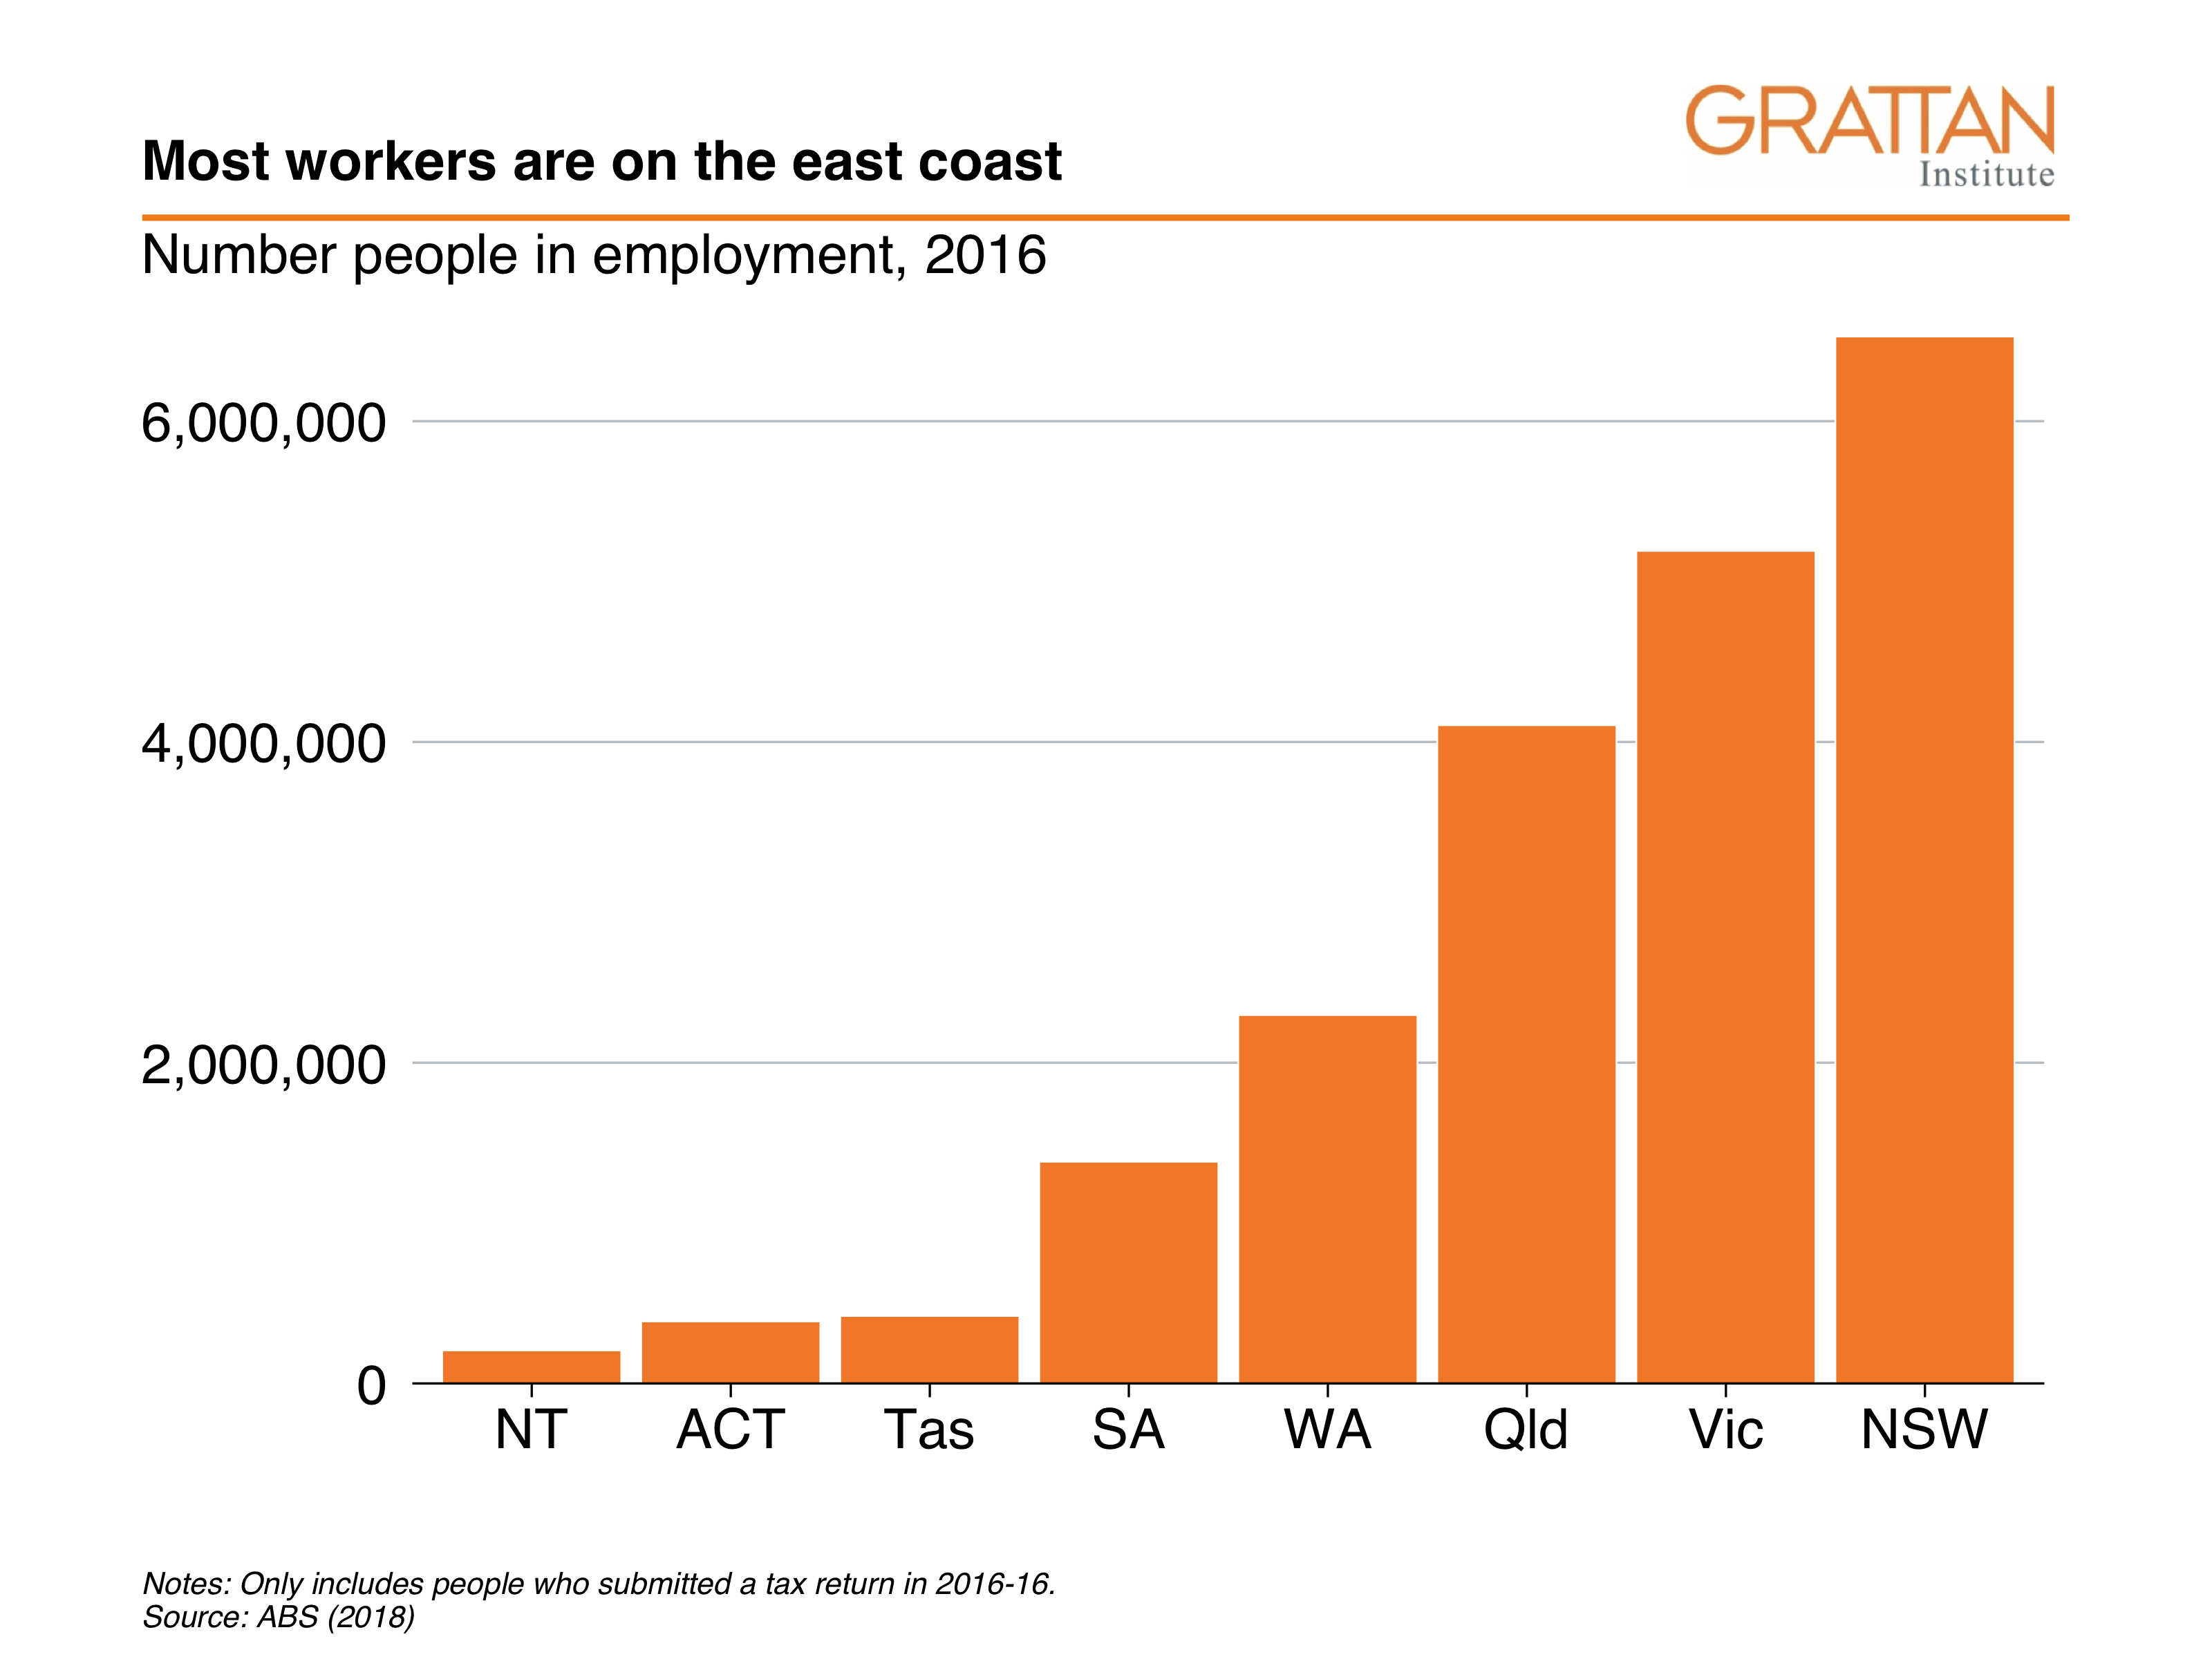
\includegraphics[width=44.44in]{atlas/simple_bar}

First, create the data you want to plot.

\begin{Shaded}
\begin{Highlighting}[]
\NormalTok{data <-}\StringTok{ }\NormalTok{sa3_income }\OperatorTok\StringTok{ }
\StringTok{  }\KeywordTok{filter}\NormalTok{(year }\OperatorTok{==}\StringTok{ }\DecValTok{2016}\NormalTok{) }\OperatorTok\StringTok{ }
\StringTok{  }\KeywordTok{group_by}\NormalTok{(state) }\OperatorTok\StringTok{ }
\StringTok{  }\KeywordTok{summarise}\NormalTok{(}\DataTypeTok{workers =} \KeywordTok{sum}\NormalTok{(workers))}

\NormalTok{data}
\end{Highlighting}
\end{Shaded}

\begin{verbatim}
## # A tibble: 8 x 2
##   state workers
##   <chr>   <dbl>
## 1 ACT    386989
## 2 NSW   6527661
## 3 NT     206061
## 4 Qld   4104503
## 5 SA    1382446
## 6 Tas    420767
## 7 Vic   5190976
## 8 WA    2297081
\end{verbatim}

Looks of the highest quality: you have one observation (row) for each state you want to plot, and a value for their number of workers.

Now pass the nice, simple table to \texttt{ggplot} and add aesthetics so that \texttt{x} represents \texttt{state}, and \texttt{y} represents \texttt{workers}. Then, because the dataset contains the \emph{actual} numbers you want on the chart, you can plot the data with \texttt{geom\_col}:\footnote{Remember that \texttt{geom\_col} is just shorthand for \texttt{geom\_bar(stat\ =\ "identity")}}

\begin{Shaded}
\begin{Highlighting}[]
\NormalTok{data }\OperatorTok\StringTok{ }
\StringTok{  }\KeywordTok{ggplot}\NormalTok{(}\KeywordTok{aes}\NormalTok{(}\DataTypeTok{x =}\NormalTok{ state,}
             \DataTypeTok{y =}\NormalTok{ workers)) }\OperatorTok{+}\StringTok{ }
\StringTok{  }\KeywordTok{geom_col}\NormalTok{()}
\end{Highlighting}
\end{Shaded}

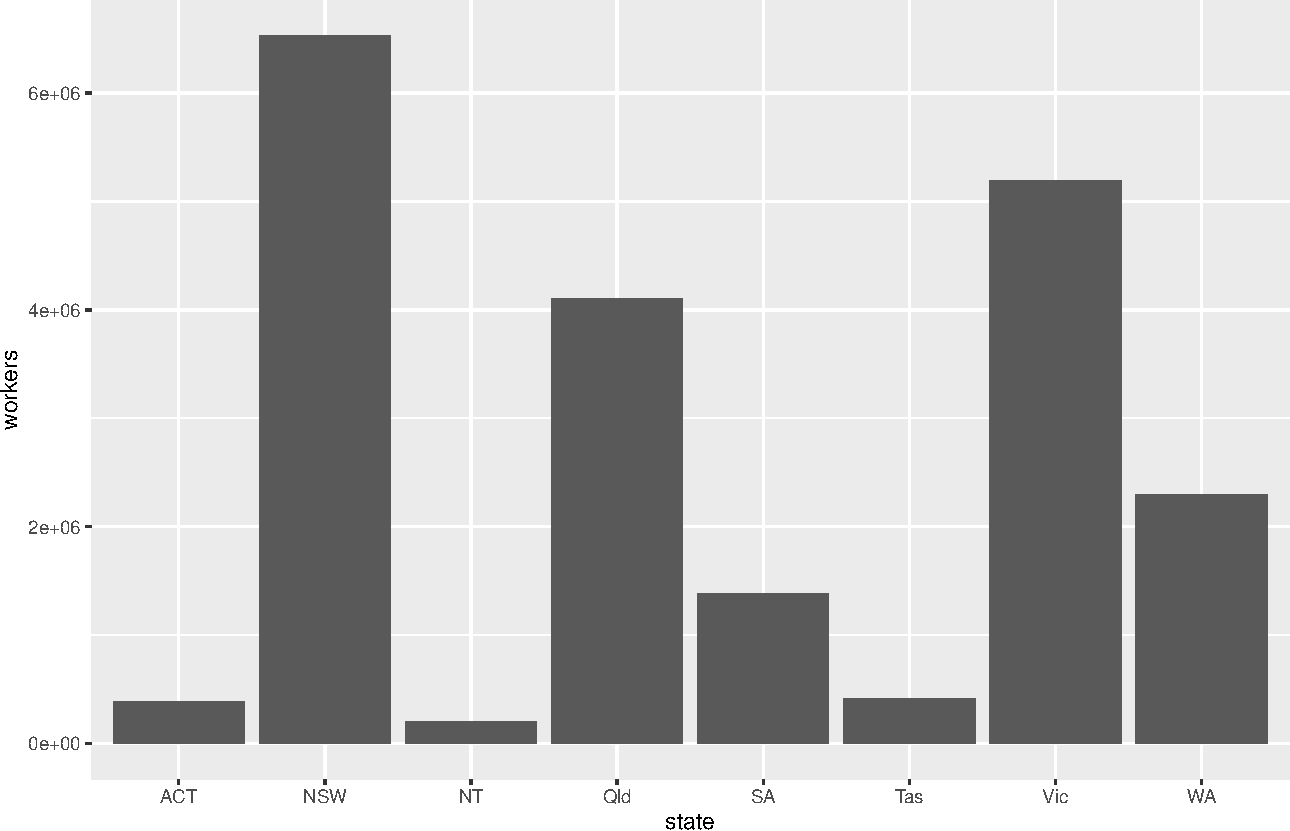
\includegraphics{Visualisation_cookbook_files/figure-latex/simple_bar_base-1.pdf}

Make it Grattany by adjusting general theme defaults with \texttt{theme\_grattan}, and use \texttt{grattan\_y\_continuous} to change the y-axis. Use labels formatted with commas (rather than scientific notation) by adding \texttt{labels\ =\ comma}.

\begin{Shaded}
\begin{Highlighting}[]
\NormalTok{data }\OperatorTok\StringTok{ }
\StringTok{  }\KeywordTok{ggplot}\NormalTok{(}\KeywordTok{aes}\NormalTok{(}\DataTypeTok{x =}\NormalTok{ state,}
             \DataTypeTok{y =}\NormalTok{ workers)) }\OperatorTok{+}\StringTok{ }
\StringTok{  }\KeywordTok{geom_col}\NormalTok{() }\OperatorTok{+}\StringTok{ }
\StringTok{  }\KeywordTok{theme_grattan}\NormalTok{() }\OperatorTok{+}\StringTok{ }
\StringTok{  }\KeywordTok{grattan_y_continuous}\NormalTok{(}\DataTypeTok{labels =}\NormalTok{ comma)}
\end{Highlighting}
\end{Shaded}

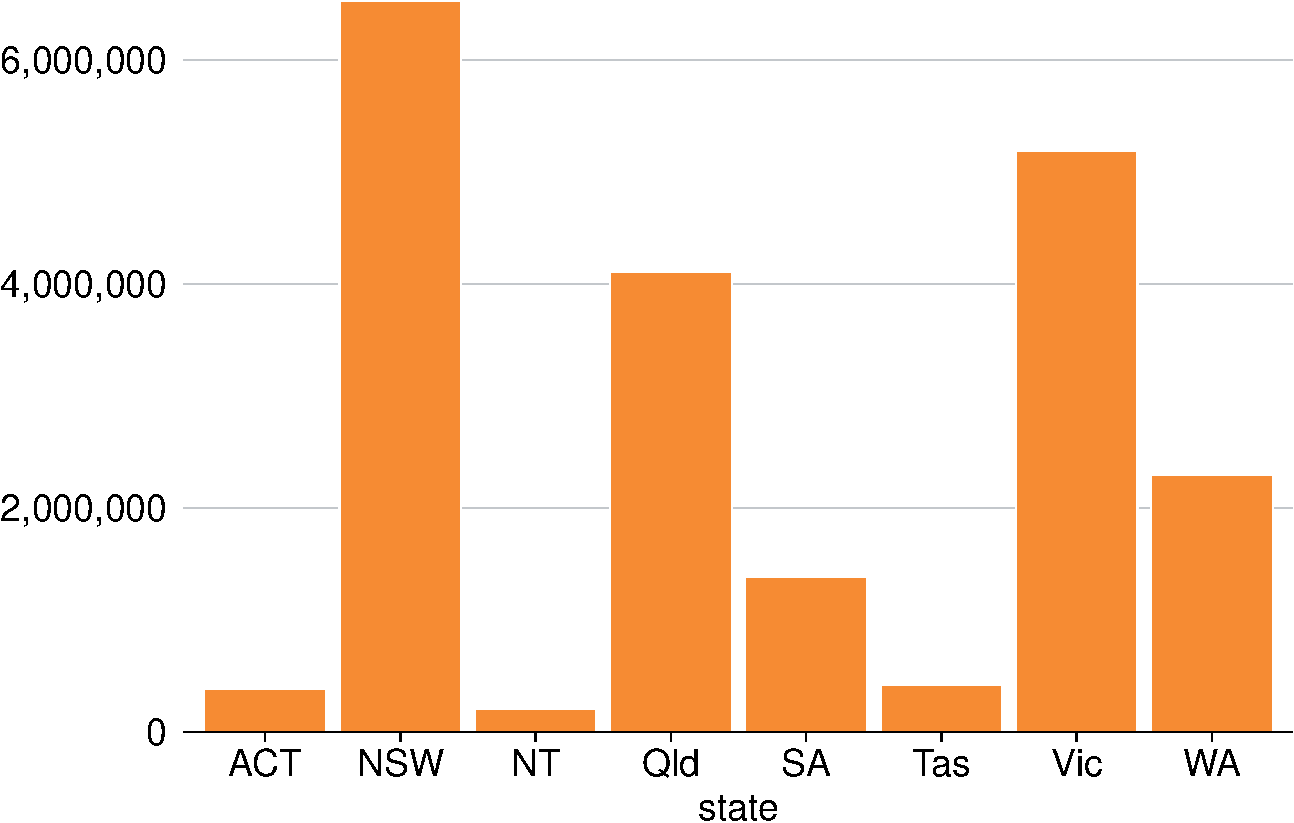
\includegraphics{Visualisation_cookbook_files/figure-latex/simple_bar_grattan-1.pdf}

To order the states by number of workers, you can tell the \texttt{x} aesthetic that you want to \texttt{reorder} the \texttt{state} variable by \texttt{workers}:

\begin{Shaded}
\begin{Highlighting}[]
\NormalTok{data }\OperatorTok\StringTok{ }
\StringTok{  }\KeywordTok{ggplot}\NormalTok{(}\KeywordTok{aes}\NormalTok{(}\DataTypeTok{x =} \KeywordTok{reorder}\NormalTok{(state, workers), }\CommentTok{# reorder states by workers}
             \DataTypeTok{y =}\NormalTok{ workers)) }\OperatorTok{+}\StringTok{ }
\StringTok{  }\KeywordTok{geom_col}\NormalTok{() }\OperatorTok{+}\StringTok{ }
\StringTok{  }\KeywordTok{theme_grattan}\NormalTok{() }\OperatorTok{+}\StringTok{ }
\StringTok{  }\KeywordTok{grattan_y_continuous}\NormalTok{(}\DataTypeTok{labels =}\NormalTok{ comma)}
\end{Highlighting}
\end{Shaded}

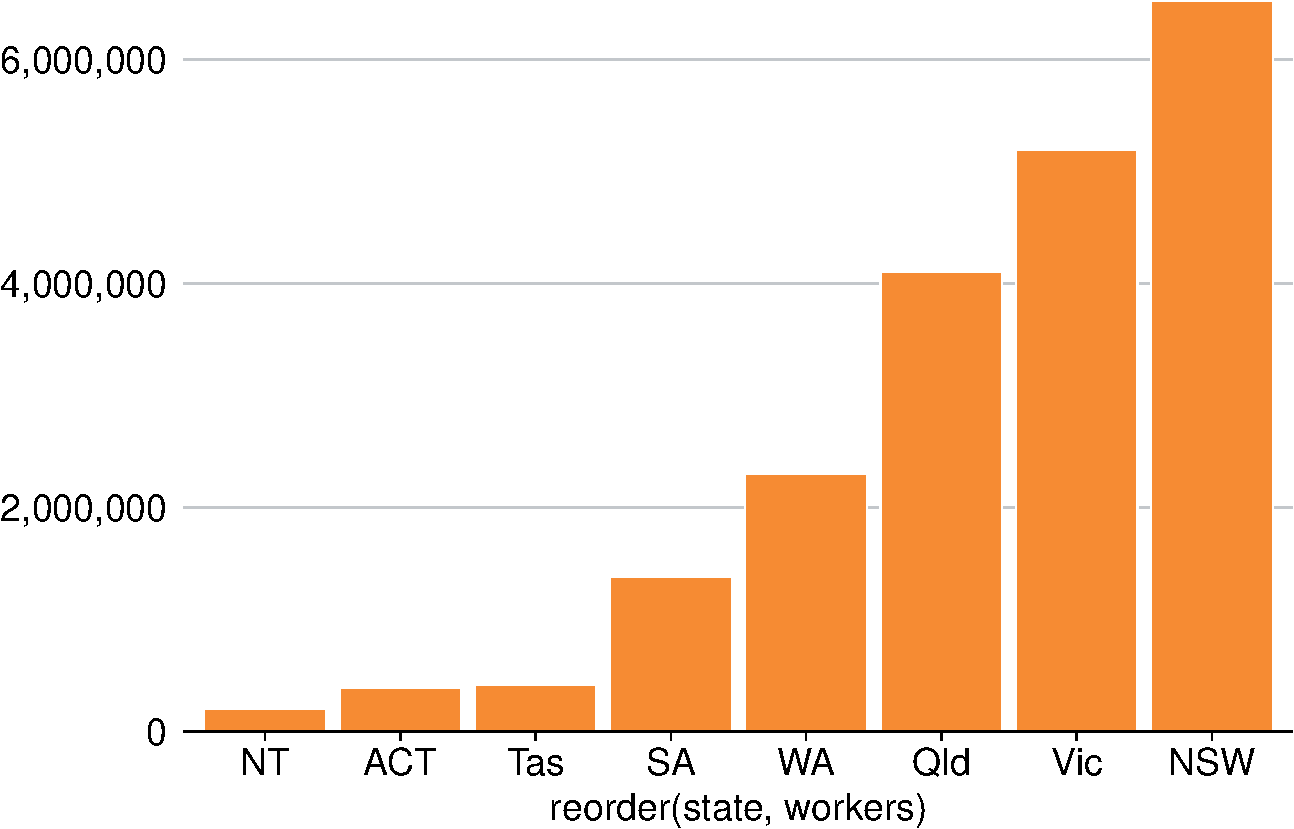
\includegraphics{Visualisation_cookbook_files/figure-latex/simple_bar_reorder-1.pdf}

You can probably drop the x-axis label -- people will understand that they're states without you explicitly saying it -- and add a title and subtitle with \texttt{labs}:

\begin{Shaded}
\begin{Highlighting}[]
\NormalTok{simple_bar <-}\StringTok{ }\NormalTok{data }\OperatorTok\StringTok{ }
\StringTok{  }\KeywordTok{ggplot}\NormalTok{(}\KeywordTok{aes}\NormalTok{(}\DataTypeTok{x =} \KeywordTok{reorder}\NormalTok{(state, workers),}
             \DataTypeTok{y =}\NormalTok{ workers)) }\OperatorTok{+}\StringTok{ }
\StringTok{  }\KeywordTok{geom_col}\NormalTok{() }\OperatorTok{+}\StringTok{ }
\StringTok{  }\KeywordTok{theme_grattan}\NormalTok{() }\OperatorTok{+}\StringTok{ }
\StringTok{  }\KeywordTok{grattan_y_continuous}\NormalTok{(}\DataTypeTok{labels =}\NormalTok{ comma) }\OperatorTok{+}\StringTok{ }
\StringTok{  }\KeywordTok{labs}\NormalTok{(}\DataTypeTok{title =} \StringTok{"Most workers are on the east coast"}\NormalTok{,}
       \DataTypeTok{subtitle =} \StringTok{"Number people in employment, 2016"}\NormalTok{,}
       \DataTypeTok{x =} \StringTok{""}\NormalTok{,}
       \DataTypeTok{caption =} \StringTok{"Notes: Only includes people who submitted a tax return in 2016-16. Source: ABS (2018)"}\NormalTok{)}

\NormalTok{simple_bar}
\end{Highlighting}
\end{Shaded}

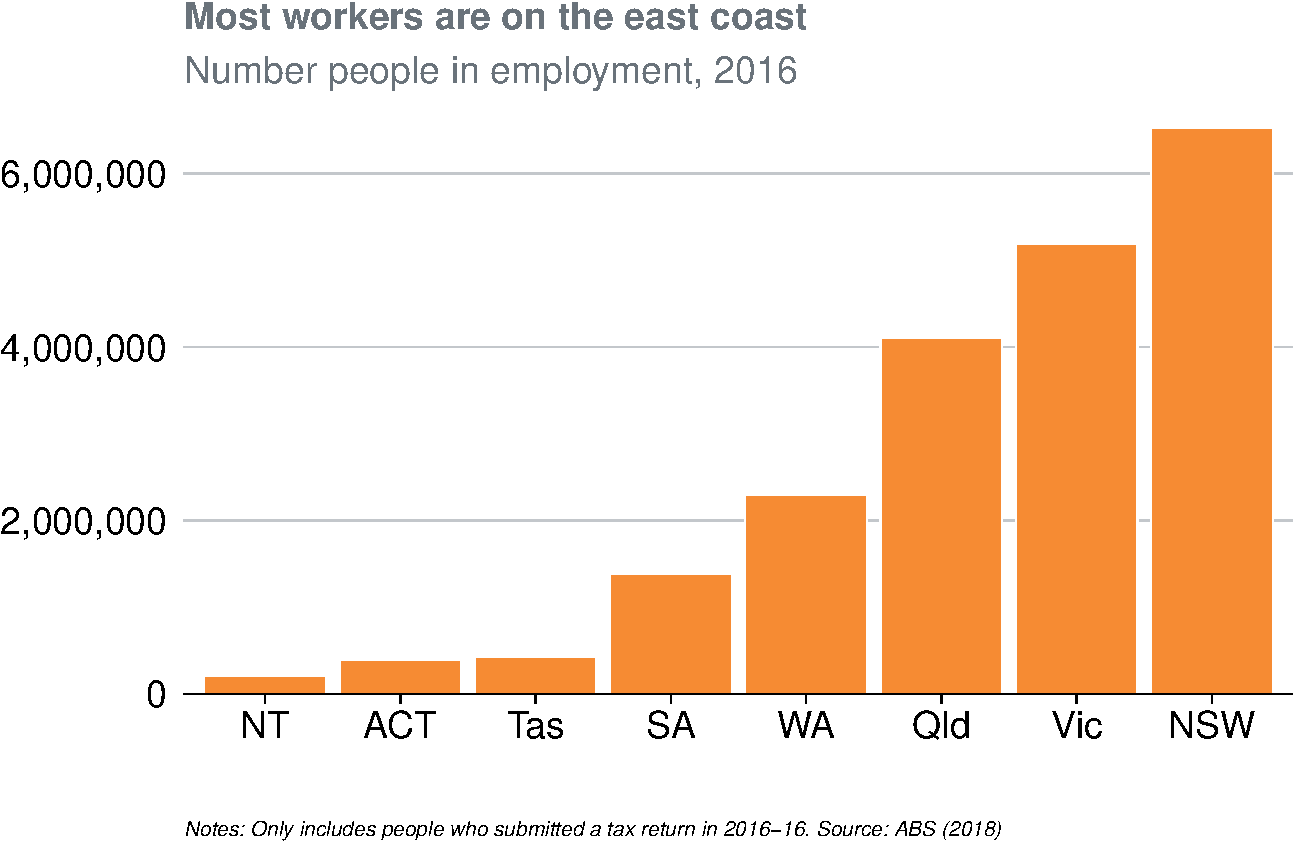
\includegraphics{Visualisation_cookbook_files/figure-latex/simple_bar_title-1.pdf}

Looks fine! Now you can export as a full-slide Grattan chart using \texttt{grattan\_save}:

\begin{Shaded}
\begin{Highlighting}[]
\KeywordTok{grattan_save}\NormalTok{(}\StringTok{"atlas/simple_bar.pdf"}\NormalTok{, simple_bar, }\DataTypeTok{type =} \StringTok{"fullslide"}\NormalTok{)}
\end{Highlighting}
\end{Shaded}

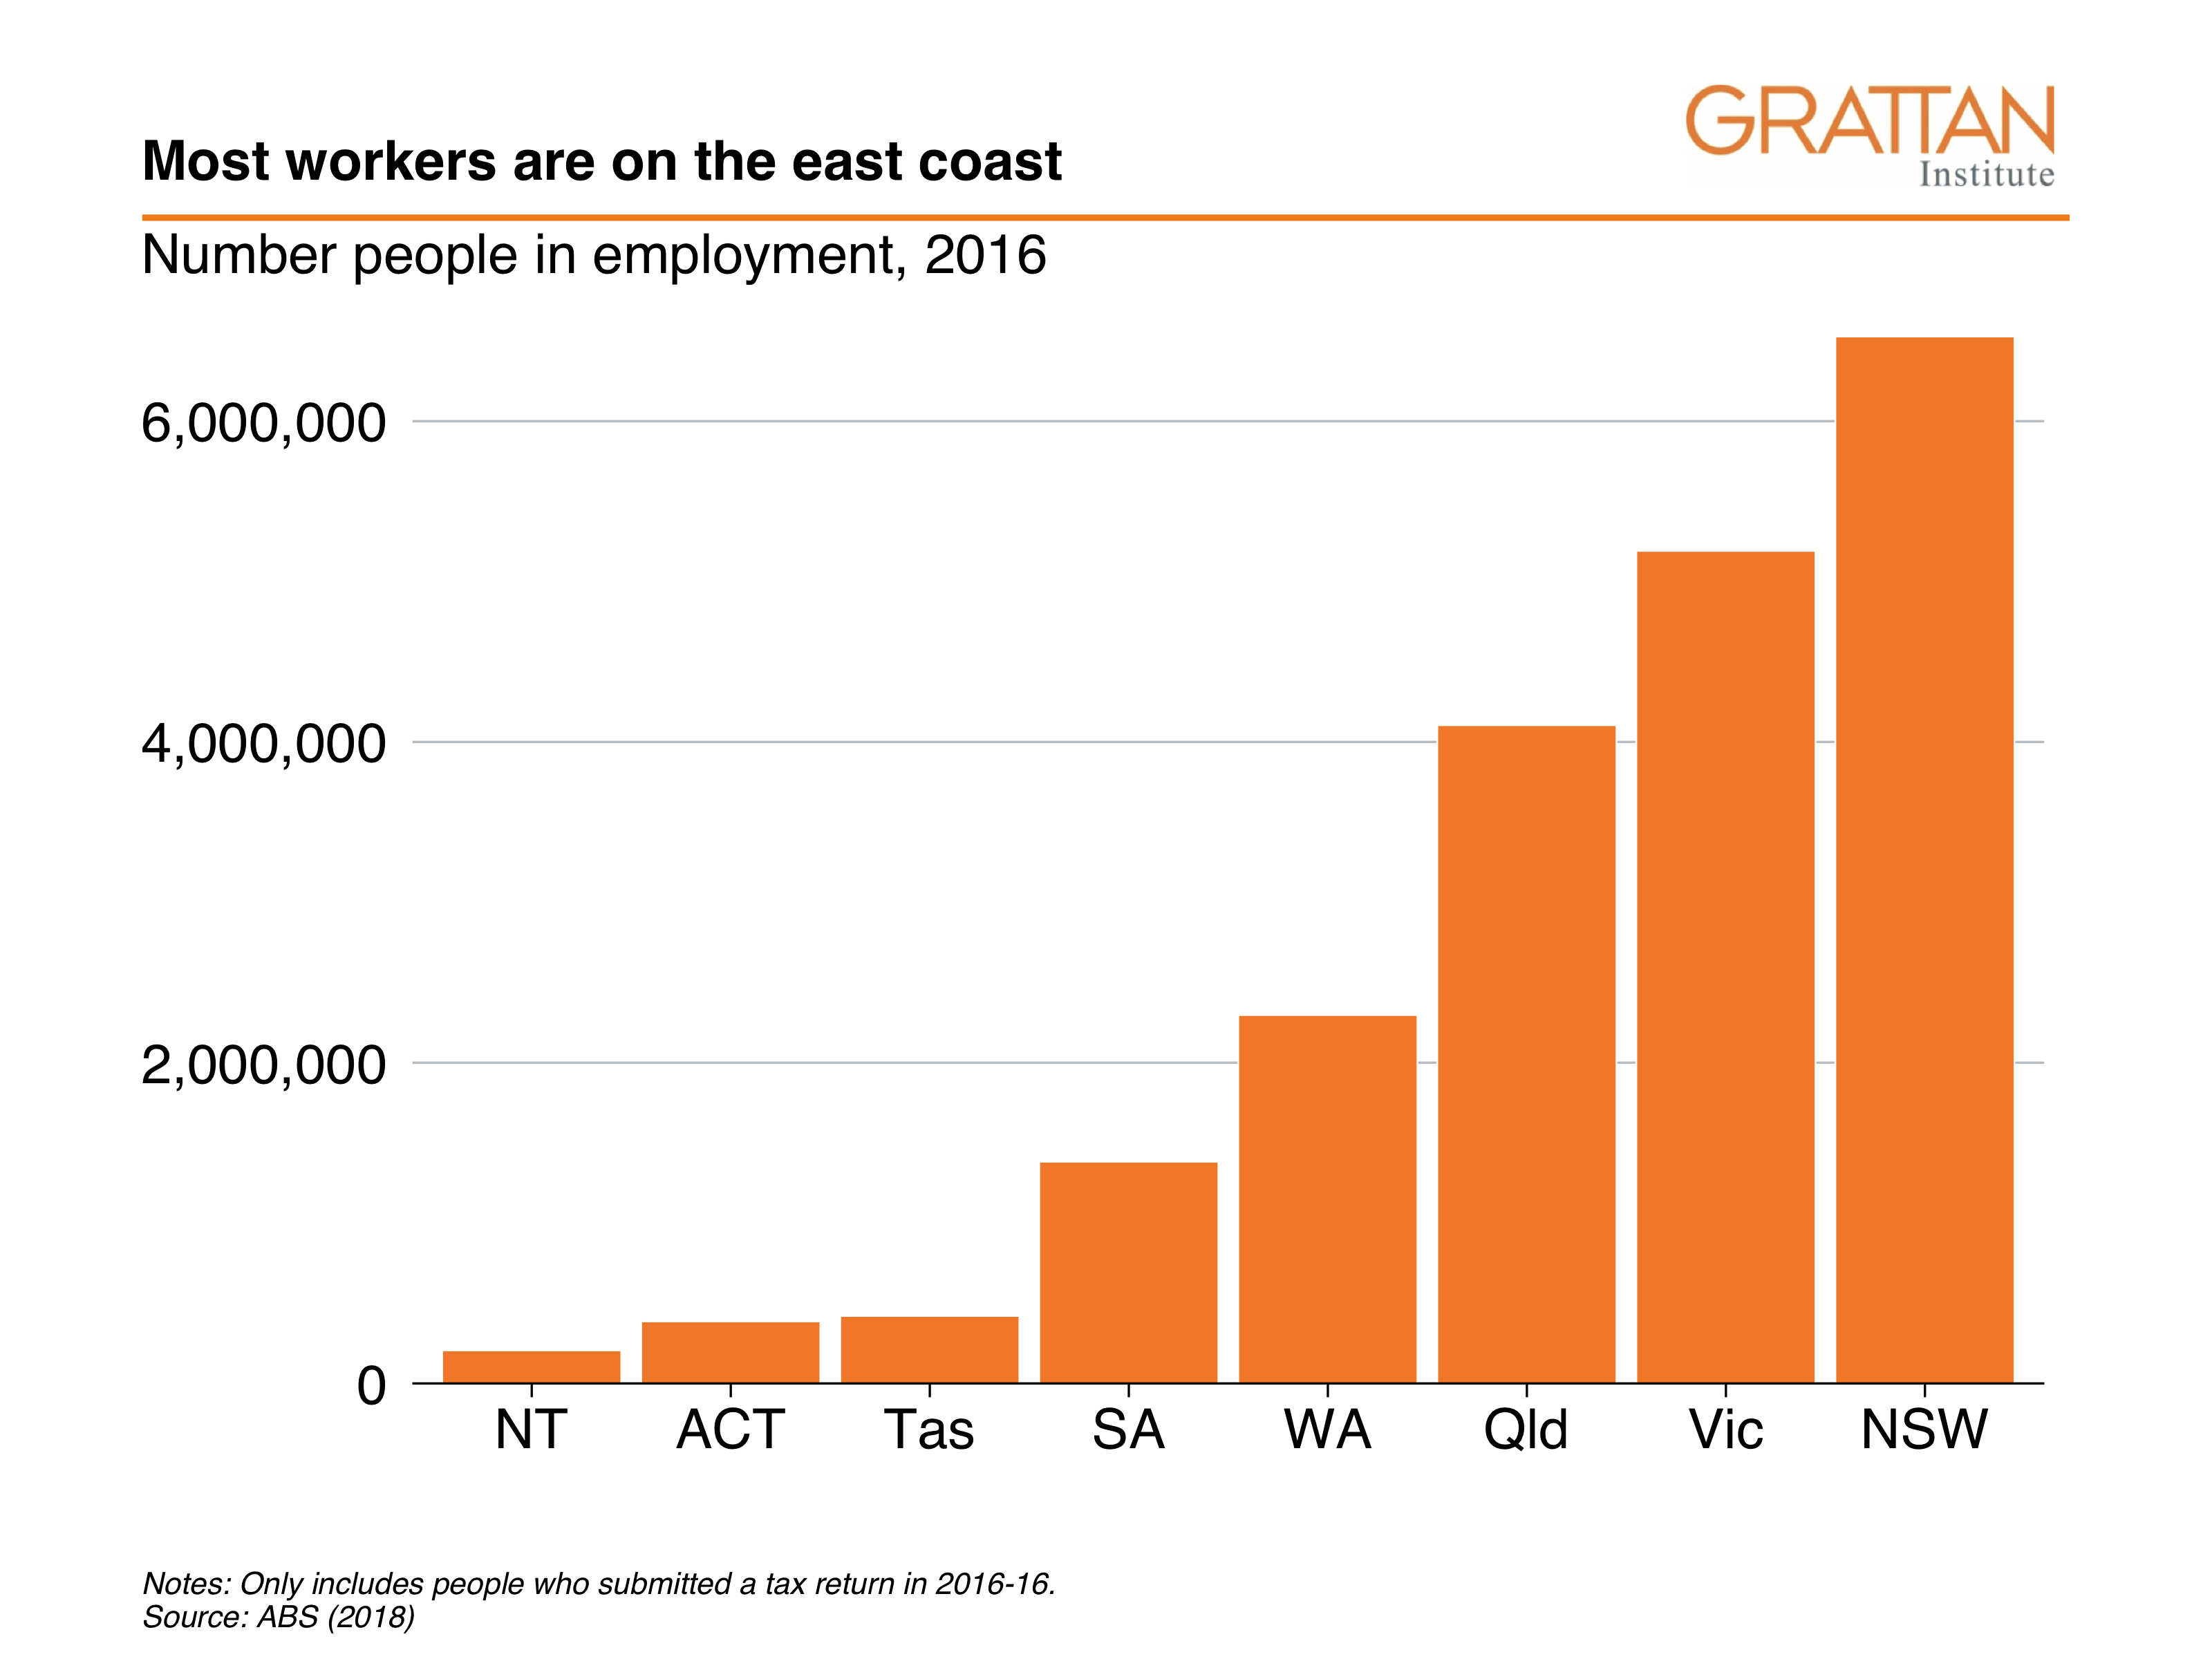
\includegraphics[width=44.44in]{atlas/simple_bar}

\hypertarget{bar-multi}{%
\subsection{Bar plot with multiple series}\label{bar-multi}}

This section will create a horizontal bar plot showing average income by state and gender in 2016:

First create the dataset you want to plot, getting the average income by state and gender in the year 2016:

\begin{Shaded}
\begin{Highlighting}[]
\NormalTok{data <-}\StringTok{ }\NormalTok{sa3_income }\OperatorTok\StringTok{ }
\StringTok{  }\KeywordTok{filter}\NormalTok{(year }\OperatorTok{==}\StringTok{ }\DecValTok{2016}\NormalTok{) }\OperatorTok\StringTok{   }
\StringTok{  }\KeywordTok{group_by}\NormalTok{(state, gender) }\OperatorTok\StringTok{   }
\StringTok{  }\KeywordTok{summarise}\NormalTok{(}\DataTypeTok{average_income =} \KeywordTok{sum}\NormalTok{(total_income) }\OperatorTok{/}\StringTok{ }\KeywordTok{sum}\NormalTok{(workers))}

\NormalTok{data}
\end{Highlighting}
\end{Shaded}

\begin{verbatim}
## # A tibble: 16 x 3
## # Groups:   state [8]
##    state gender average_income
##    <chr> <chr>           <dbl>
##  1 ACT   Men            78141.
##  2 ACT   Women          65548.
##  3 NSW   Men            69750.
##  4 NSW   Women          53191.
##  5 NT    Men            75246.
##  6 NT    Women          58527.
##  7 Qld   Men            65108.
##  8 Qld   Women          48458.
##  9 SA    Men            60244.
## 10 SA    Women          47533.
## 11 Tas   Men            56345.
## 12 Tas   Women          45158.
## 13 Vic   Men            64908.
## 14 Vic   Women          49264.
## 15 WA    Men            76677.
## 16 WA    Women          51578.
\end{verbatim}

Looks fine: you have one observation (row) for each state \(\times\) gender group you want to plot, and a value for their average income. Put \texttt{state} on the x-axis, \texttt{average\_income} on the y-axis, and split gender by fill-colour (\texttt{fill}).

Pass the data to \texttt{ggplot}, give it the appropriate \texttt{x} and \texttt{y} aesthetics, along with \texttt{fill} (the fill colour\footnote{The aesthetic \texttt{fill} represents the `fill' colour -- the colour that fills the bars in your chart. The \texttt{colour} aesthetic controls the colours of the \emph{lines}.}) representing \texttt{gender}. And because you have the \emph{actual} values for \texttt{average\_income} you want to plot, use \texttt{geom\_col}:\footnote{\texttt{geom\_col} is shorthand for \texttt{geom\_bar(stat\ =\ "identity"}}

\begin{Shaded}
\begin{Highlighting}[]
\NormalTok{data }\OperatorTok\StringTok{ }
\StringTok{  }\KeywordTok{ggplot}\NormalTok{(}\KeywordTok{aes}\NormalTok{(}\DataTypeTok{x =}\NormalTok{ state,}
             \DataTypeTok{y =}\NormalTok{ average_income,}
             \DataTypeTok{fill =}\NormalTok{ gender)) }\OperatorTok{+}\StringTok{ }
\StringTok{  }\KeywordTok{geom_col}\NormalTok{()}
\end{Highlighting}
\end{Shaded}

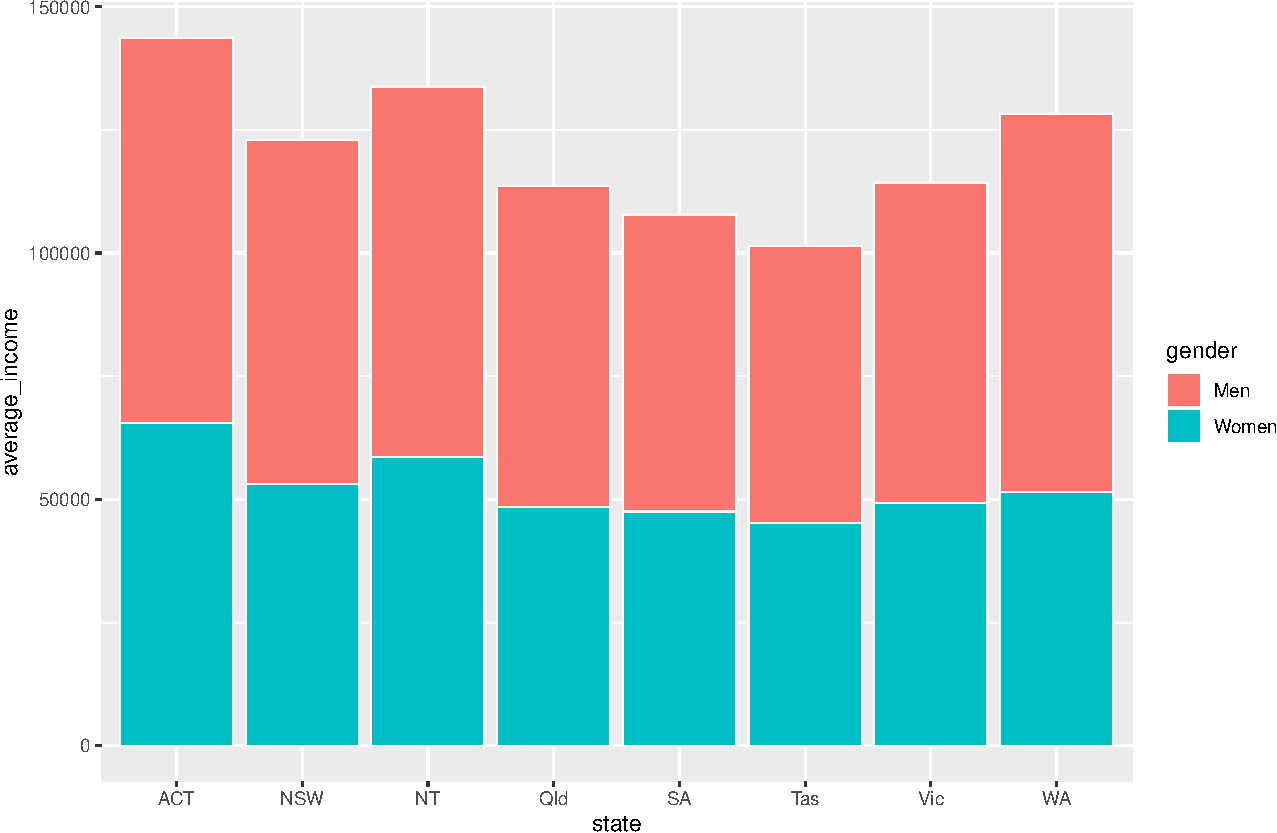
\includegraphics{Visualisation_cookbook_files/figure-latex/bar_multi_base-1.pdf}

The two series -- women and men -- created by \texttt{fill} are stacked on-top of each other by \texttt{geom\_col}. You can tell it to plot them next to each other -- to `dodge' -- instead with the \texttt{position} argument \emph{within} \texttt{geom\_col}:

\begin{Shaded}
\begin{Highlighting}[]
\NormalTok{data }\OperatorTok\StringTok{ }
\StringTok{  }\KeywordTok{ggplot}\NormalTok{(}\KeywordTok{aes}\NormalTok{(}\DataTypeTok{x =}\NormalTok{ state,}
             \DataTypeTok{y =}\NormalTok{ average_income,}
             \DataTypeTok{fill =}\NormalTok{ gender)) }\OperatorTok{+}\StringTok{ }
\StringTok{  }\KeywordTok{geom_col}\NormalTok{(}\DataTypeTok{position =} \StringTok{"dodge"}\NormalTok{) }\CommentTok{# 'dodge' the series}
\end{Highlighting}
\end{Shaded}

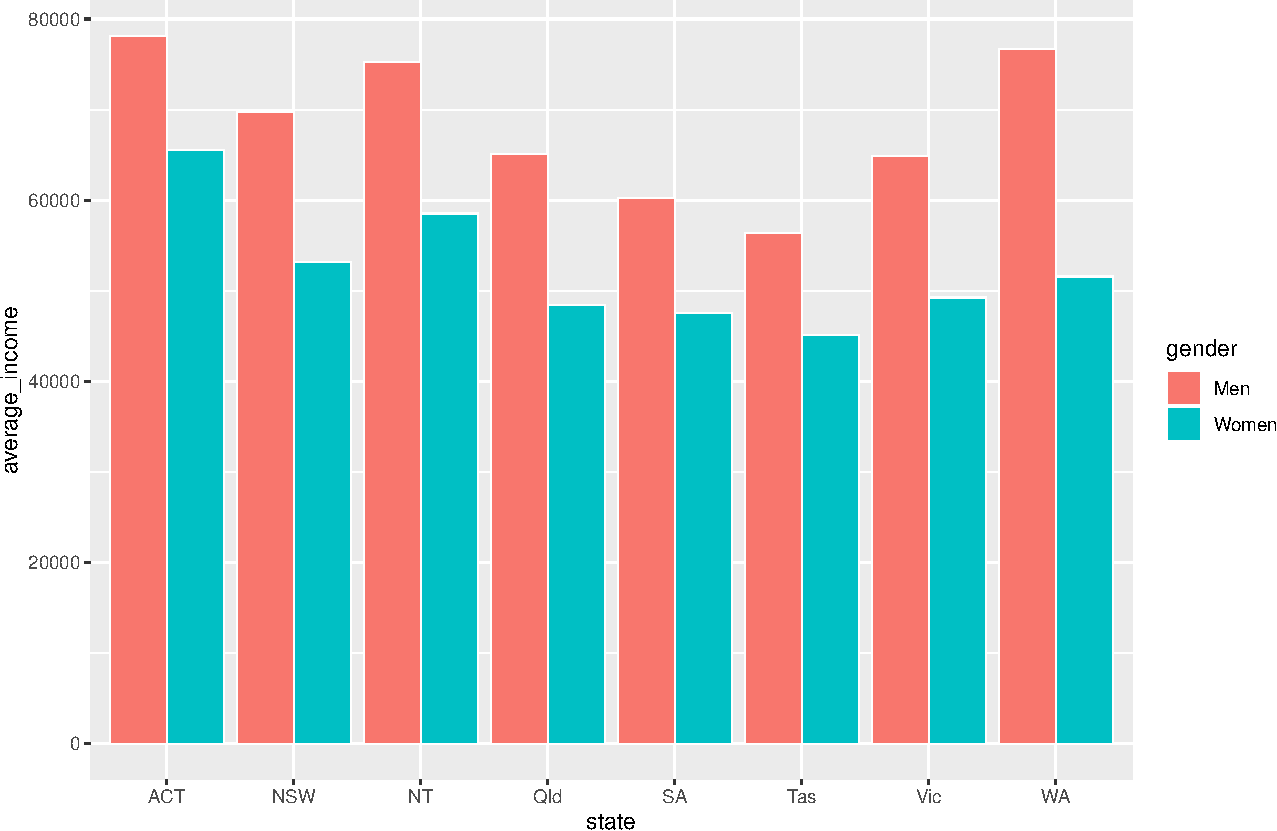
\includegraphics{Visualisation_cookbook_files/figure-latex/bar_multi_dodge-1.pdf}

To flip the chart -- a useful move when you have long labels -- add \texttt{coord\_flip} (ie `flip the x and y coordinates of the chart').

However, while the \emph{coordinates} have been flipped, the underlying data hasn't. If you want to refer to the \texttt{average\_income} axis, which now lies horizontally, you would still refer to the \texttt{y} axis (eg \texttt{grattan\_y\_continuous} still refers to your \texttt{y} aesthetic, \texttt{average\_income}).

\begin{Shaded}
\begin{Highlighting}[]
\NormalTok{data }\OperatorTok\StringTok{ }
\StringTok{  }\KeywordTok{ggplot}\NormalTok{(}\KeywordTok{aes}\NormalTok{(}\DataTypeTok{x =}\NormalTok{ state,}
             \DataTypeTok{y =}\NormalTok{ average_income,}
             \DataTypeTok{fill =}\NormalTok{ gender)) }\OperatorTok{+}\StringTok{ }
\StringTok{  }\KeywordTok{geom_col}\NormalTok{(}\DataTypeTok{position =} \StringTok{"dodge"}\NormalTok{) }\OperatorTok{+}\StringTok{ }
\StringTok{  }\KeywordTok{coord_flip}\NormalTok{() }\CommentTok{# rotate the chart}
\end{Highlighting}
\end{Shaded}

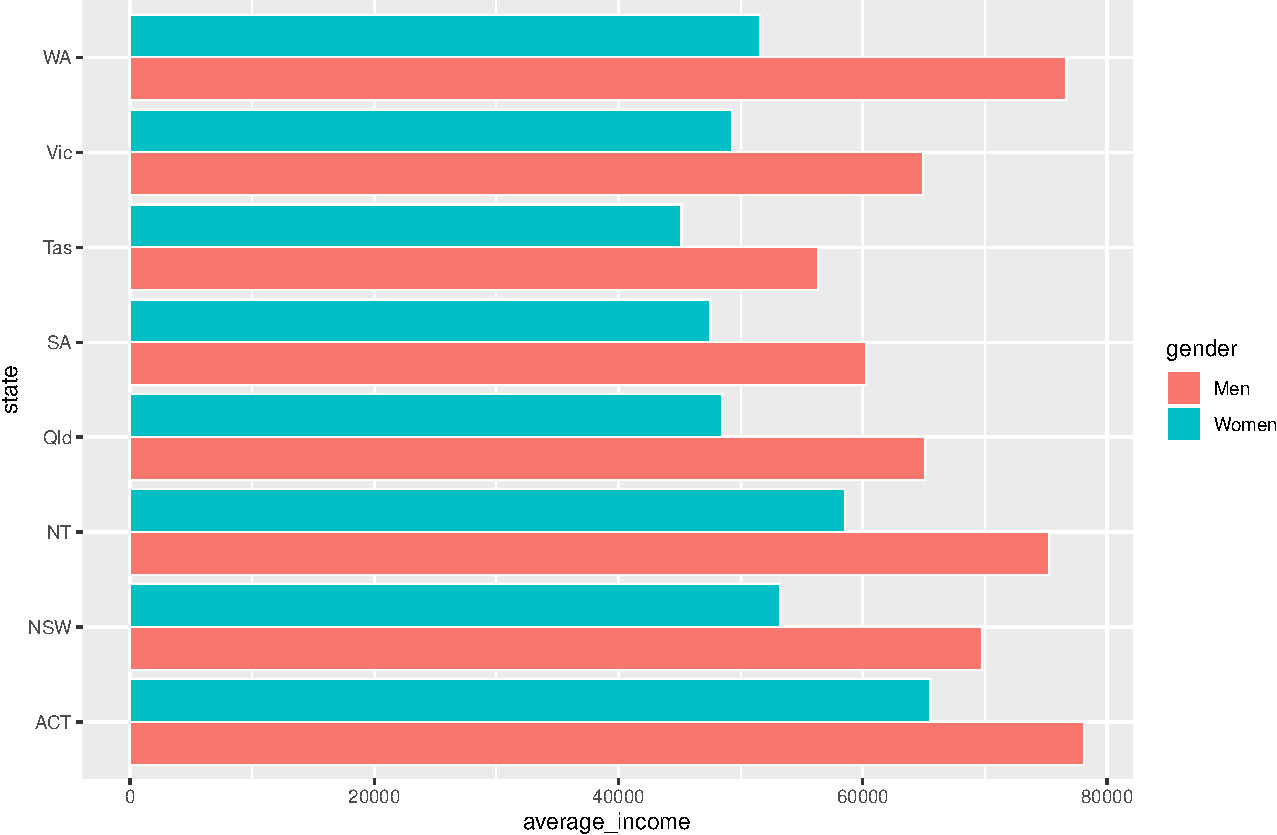
\includegraphics{Visualisation_cookbook_files/figure-latex/bar_multi_flip-1.pdf}

And reorder the states by average income, so that the state with the highest (combined) average income is at the top. This is done with the \texttt{reorder(var\_to\_reorder,\ var\_to\_reorder\_by)} function when you define the \texttt{state} aesthetic:

\begin{Shaded}
\begin{Highlighting}[]
\NormalTok{data }\OperatorTok\StringTok{ }
\StringTok{  }\KeywordTok{ggplot}\NormalTok{(}\KeywordTok{aes}\NormalTok{(}\DataTypeTok{x =} \KeywordTok{reorder}\NormalTok{(state, average_income), }\CommentTok{# reorder}
             \DataTypeTok{y =}\NormalTok{ average_income,}
             \DataTypeTok{fill =}\NormalTok{ gender)) }\OperatorTok{+}\StringTok{ }
\StringTok{  }\KeywordTok{geom_col}\NormalTok{(}\DataTypeTok{position =} \StringTok{"dodge"}\NormalTok{) }\OperatorTok{+}\StringTok{ }
\StringTok{  }\KeywordTok{coord_flip}\NormalTok{()}
\end{Highlighting}
\end{Shaded}

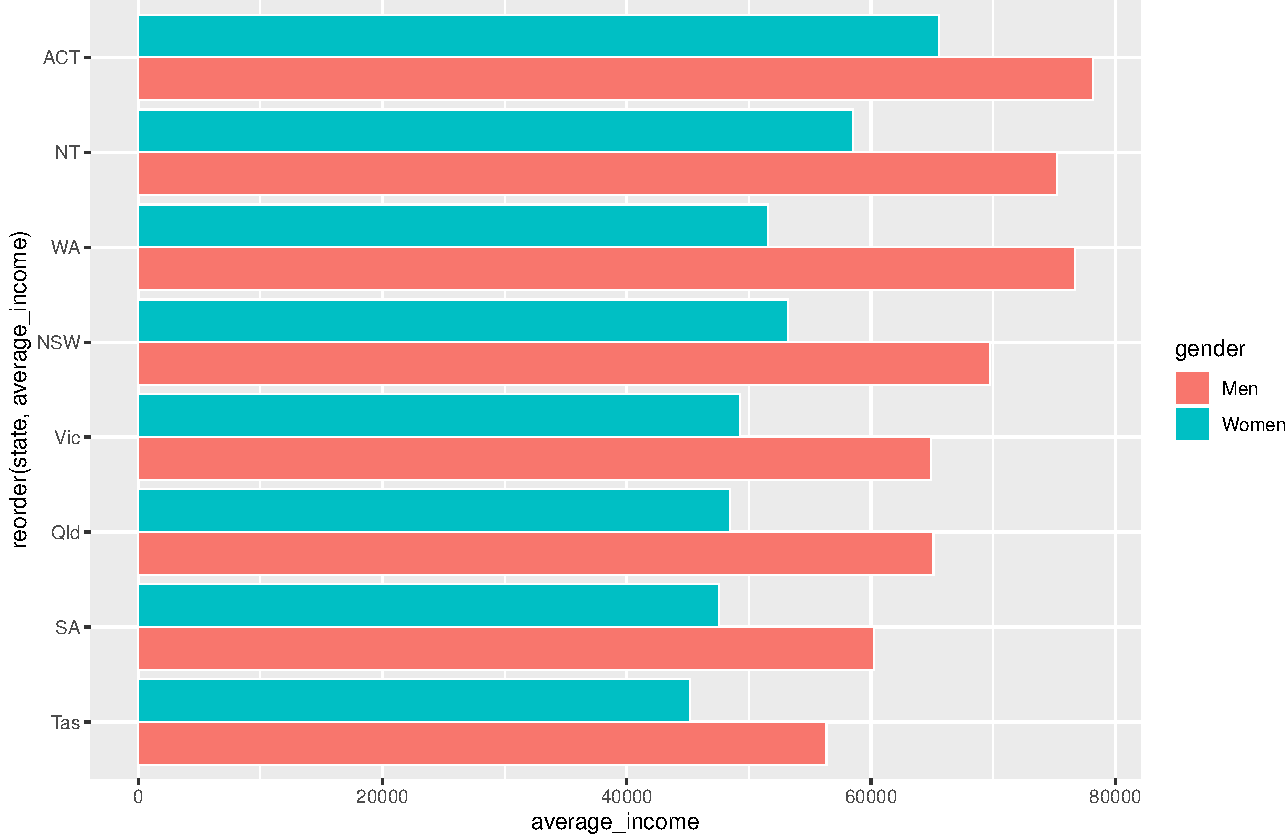
\includegraphics{Visualisation_cookbook_files/figure-latex/bar_multi_reorder-1.pdf}

Wonderful -- that's how you want our \emph{data} to look. Now you can Grattanise it. Note that \texttt{theme\_grattan} needs to know that the coordinates were flipped so it can apply the right settings. Also tell \texttt{grattan\_fill\_manual} that there are two fill series.

\begin{Shaded}
\begin{Highlighting}[]
\NormalTok{data }\OperatorTok\StringTok{ }
\StringTok{  }\KeywordTok{ggplot}\NormalTok{(}\KeywordTok{aes}\NormalTok{(}\DataTypeTok{x =} \KeywordTok{reorder}\NormalTok{(state, average_income), }
             \DataTypeTok{y =}\NormalTok{ average_income,}
             \DataTypeTok{fill =}\NormalTok{ gender)) }\OperatorTok{+}\StringTok{ }
\StringTok{  }\KeywordTok{geom_col}\NormalTok{(}\DataTypeTok{position =} \StringTok{"dodge"}\NormalTok{) }\OperatorTok{+}\StringTok{ }
\StringTok{  }\KeywordTok{coord_flip}\NormalTok{() }\OperatorTok{+}\StringTok{ }
\StringTok{  }\KeywordTok{theme_grattan}\NormalTok{(}\DataTypeTok{flipped =} \OtherTok{TRUE}\NormalTok{) }\OperatorTok{+}\StringTok{ }\CommentTok{# grattan theme}
\StringTok{  }\KeywordTok{grattan_y_continuous}\NormalTok{(}\DataTypeTok{labels =}\NormalTok{ dollar) }\OperatorTok{+}\StringTok{ }\CommentTok{# y axis}
\StringTok{  }\KeywordTok{grattan_fill_manual}\NormalTok{(}\DecValTok{2}\NormalTok{) }\CommentTok{# grattan fill colours}
\end{Highlighting}
\end{Shaded}

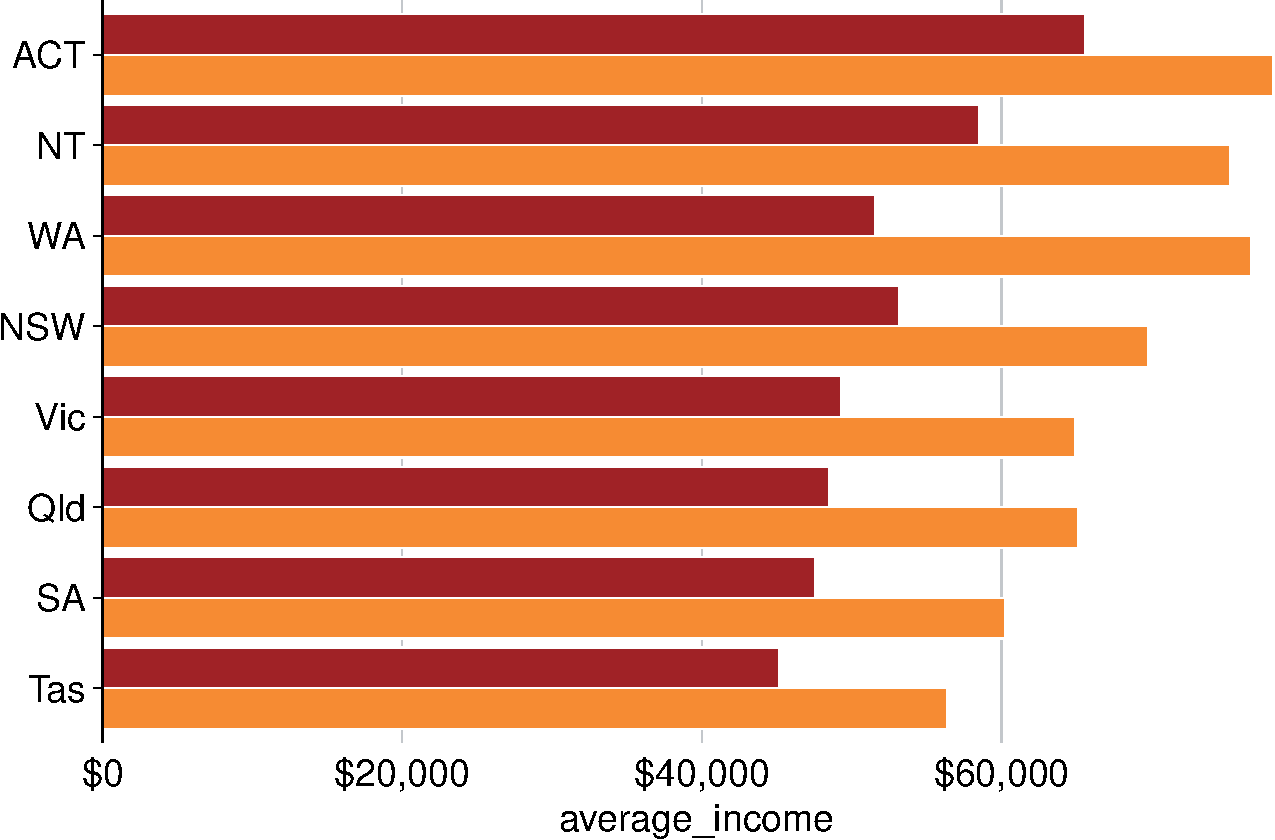
\includegraphics{Visualisation_cookbook_files/figure-latex/bar_multi_grattan-1.pdf}

You can use \texttt{grattan\_label} to \textbf{label your charts} in the Grattan style. This function is a `wrapper' around \texttt{geom\_label} that has settings that we tend to like: white background with a thin margin, 18-point font, and no border. It takes the \href{https://ggplot2.tidyverse.org/reference/geom_text.html}{standard arguments of \texttt{geom\_label}}.

Section \ref{adding-labels} shows how labels are treated like data points: they need to know where to go (\texttt{x} and \texttt{y}) and what to show (\texttt{label}). But if you provide \emph{every point} to your labelling \texttt{geom}, it will plot every label:

\begin{Shaded}
\begin{Highlighting}[]
\NormalTok{data }\OperatorTok\StringTok{ }
\StringTok{  }\KeywordTok{ggplot}\NormalTok{(}\KeywordTok{aes}\NormalTok{(}\DataTypeTok{x =} \KeywordTok{reorder}\NormalTok{(state, average_income), }
             \DataTypeTok{y =}\NormalTok{ average_income,}
             \DataTypeTok{fill =}\NormalTok{ gender)) }\OperatorTok{+}\StringTok{ }
\StringTok{  }\KeywordTok{geom_col}\NormalTok{(}\DataTypeTok{position =} \StringTok{"dodge"}\NormalTok{) }\OperatorTok{+}\StringTok{ }
\StringTok{  }\KeywordTok{coord_flip}\NormalTok{() }\OperatorTok{+}\StringTok{ }
\StringTok{  }\KeywordTok{theme_grattan}\NormalTok{(}\DataTypeTok{flipped =} \OtherTok{TRUE}\NormalTok{) }\OperatorTok{+}\StringTok{ }
\StringTok{  }\KeywordTok{grattan_y_continuous}\NormalTok{(}\DataTypeTok{labels =}\NormalTok{ dollar) }\OperatorTok{+}\StringTok{ }
\StringTok{  }\KeywordTok{grattan_fill_manual}\NormalTok{(}\DecValTok{2}\NormalTok{) }\OperatorTok{+}\StringTok{ }
\StringTok{  }\KeywordTok{grattan_label}\NormalTok{(}\KeywordTok{aes}\NormalTok{(}\DataTypeTok{colour =}\NormalTok{ gender,  }\CommentTok{# colour the text according to gender}
                    \DataTypeTok{label =}\NormalTok{ gender),  }\CommentTok{# label the text according to gender}
            \DataTypeTok{position =} \KeywordTok{position_dodge}\NormalTok{(}\DataTypeTok{width =} \DecValTok{1}\NormalTok{),  }\CommentTok{# position dodge with width 1}
            \DataTypeTok{hjust =} \FloatTok{-0.1}\NormalTok{) }\OperatorTok{+}\StringTok{  }\CommentTok{# horizontally align the label so its outside the bar}
\StringTok{  }\KeywordTok{grattan_colour_manual}\NormalTok{(}\DecValTok{2}\NormalTok{)   }\CommentTok{# define colour as two grattan colours}
\end{Highlighting}
\end{Shaded}

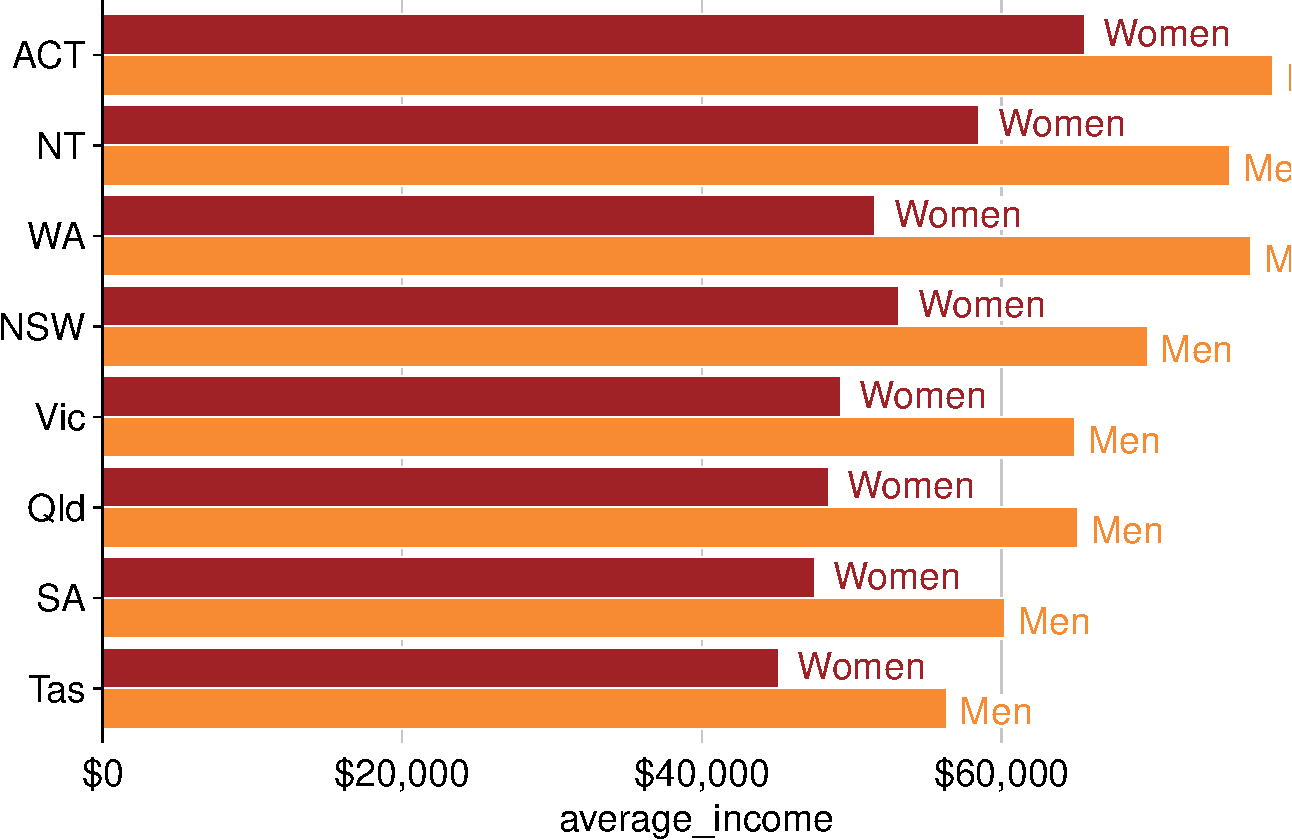
\includegraphics{Visualisation_cookbook_files/figure-latex/bar_multi_label_all-1.pdf}

To just label \emph{one} of the plots -- ie the first one, ACT in this case -- we need to tell \texttt{grattan\_label}. The easiest way to do this is by \textbf{creating a label dataset beforehand}, like \texttt{label\_gender} below. This just includes the observations you want to label:

\begin{Shaded}
\begin{Highlighting}[]
\NormalTok{label_gender <-}\StringTok{ }\NormalTok{data }\OperatorTok\StringTok{ }
\StringTok{  }\KeywordTok{filter}\NormalTok{(state }\OperatorTok{==}\StringTok{ "ACT"}\NormalTok{)  }\CommentTok{# just want Tasmania observations}

\NormalTok{label_gender}
\end{Highlighting}
\end{Shaded}

\begin{verbatim}
## # A tibble: 2 x 3
## # Groups:   state [1]
##   state gender average_income
##   <chr> <chr>           <dbl>
## 1 ACT   Men            78141.
## 2 ACT   Women          65548.
\end{verbatim}

So you can pass that \texttt{label\_gender} dataset to \texttt{grattan\_label}:

\begin{Shaded}
\begin{Highlighting}[]
\NormalTok{data }\OperatorTok\StringTok{ }
\StringTok{  }\KeywordTok{ggplot}\NormalTok{(}\KeywordTok{aes}\NormalTok{(}\DataTypeTok{x =} \KeywordTok{reorder}\NormalTok{(state, average_income), }
             \DataTypeTok{y =}\NormalTok{ average_income,}
             \DataTypeTok{fill =}\NormalTok{ gender)) }\OperatorTok{+}\StringTok{ }
\StringTok{  }\KeywordTok{geom_col}\NormalTok{(}\DataTypeTok{position =} \StringTok{"dodge"}\NormalTok{) }\OperatorTok{+}\StringTok{ }
\StringTok{  }\KeywordTok{coord_flip}\NormalTok{() }\OperatorTok{+}\StringTok{ }
\StringTok{  }\KeywordTok{theme_grattan}\NormalTok{(}\DataTypeTok{flipped =} \OtherTok{TRUE}\NormalTok{) }\OperatorTok{+}\StringTok{ }
\StringTok{  }\KeywordTok{grattan_y_continuous}\NormalTok{(}\DataTypeTok{labels =}\NormalTok{ dollar) }\OperatorTok{+}\StringTok{ }
\StringTok{  }\KeywordTok{grattan_fill_manual}\NormalTok{(}\DecValTok{2}\NormalTok{) }\OperatorTok{+}\StringTok{ }
\StringTok{  }\KeywordTok{grattan_label}\NormalTok{(}\DataTypeTok{data =}\NormalTok{ label_gender,  }\CommentTok{# supply the new dataset}
                \KeywordTok{aes}\NormalTok{(}\DataTypeTok{colour =}\NormalTok{ gender,}
                    \DataTypeTok{label =}\NormalTok{ gender), }
                \DataTypeTok{position =} \KeywordTok{position_dodge}\NormalTok{(}\DataTypeTok{width =} \DecValTok{1}\NormalTok{), }
                \DataTypeTok{hjust =} \FloatTok{-0.1}\NormalTok{) }\OperatorTok{+}\StringTok{ }
\StringTok{  }\KeywordTok{grattan_colour_manual}\NormalTok{(}\DecValTok{2}\NormalTok{)}
\end{Highlighting}
\end{Shaded}

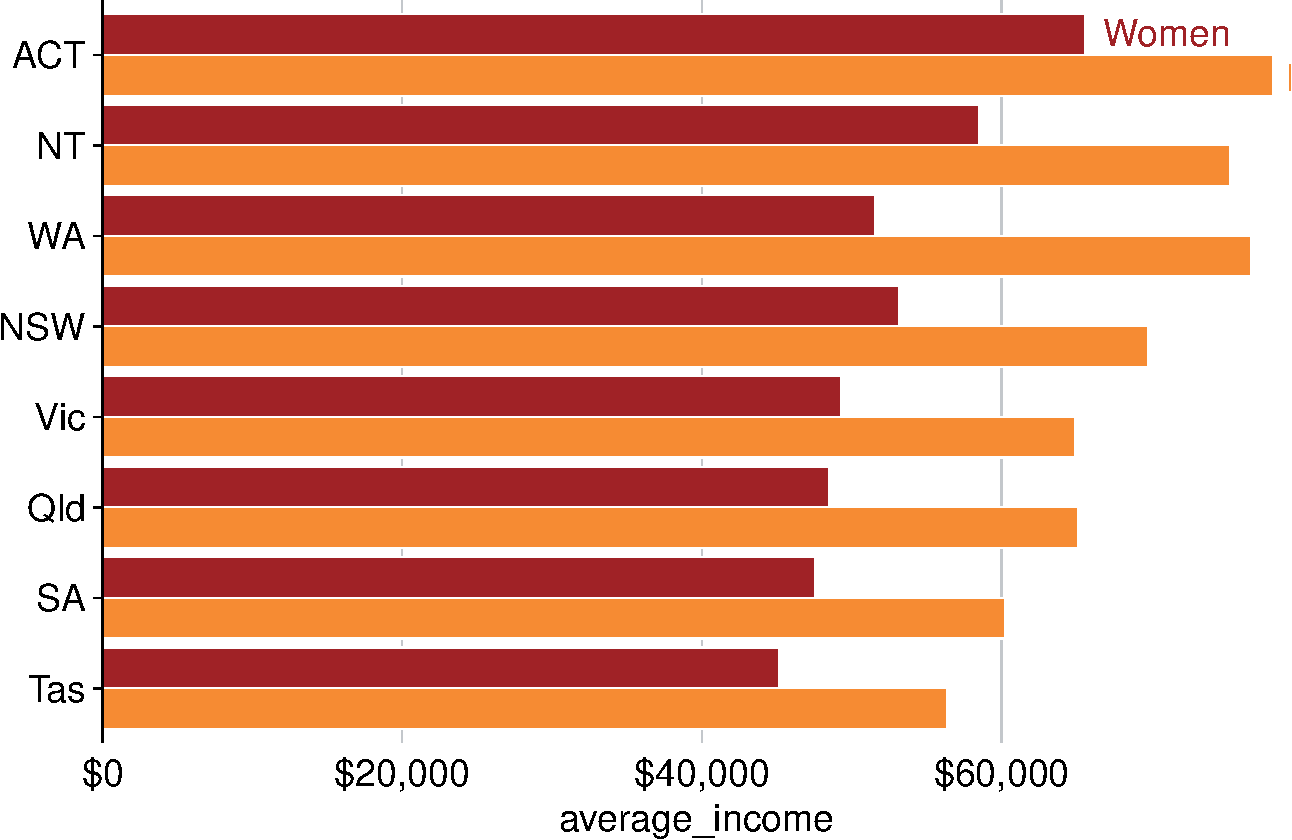
\includegraphics{Visualisation_cookbook_files/figure-latex/bar_multi_label-1.pdf}

Almost there! The labels go out of range a little bit, and we can fix this by expanding the plot:

\begin{Shaded}
\begin{Highlighting}[]
\NormalTok{data }\OperatorTok\StringTok{ }
\StringTok{  }\KeywordTok{ggplot}\NormalTok{(}\KeywordTok{aes}\NormalTok{(}\DataTypeTok{x =} \KeywordTok{reorder}\NormalTok{(state, average_income),}
             \DataTypeTok{y =}\NormalTok{ average_income,}
             \DataTypeTok{fill =}\NormalTok{ gender)) }\OperatorTok{+}\StringTok{ }
\StringTok{  }\KeywordTok{geom_col}\NormalTok{(}\DataTypeTok{position =} \StringTok{"dodge"}\NormalTok{) }\OperatorTok{+}\StringTok{ }
\StringTok{  }\KeywordTok{coord_flip}\NormalTok{() }\OperatorTok{+}\StringTok{ }
\StringTok{  }\KeywordTok{theme_grattan}\NormalTok{(}\DataTypeTok{flipped =} \OtherTok{TRUE}\NormalTok{) }\OperatorTok{+}\StringTok{ }
\StringTok{  }\KeywordTok{grattan_y_continuous}\NormalTok{(}\DataTypeTok{labels =}\NormalTok{ dollar, }
                       \DataTypeTok{expand_top =} \FloatTok{.1}\NormalTok{) }\OperatorTok{+}\StringTok{ }\CommentTok{# expand the plot}
\StringTok{  }\KeywordTok{grattan_fill_manual}\NormalTok{(}\DecValTok{2}\NormalTok{) }\OperatorTok{+}\StringTok{ }
\StringTok{  }\KeywordTok{grattan_label}\NormalTok{(}\DataTypeTok{data =}\NormalTok{ label_gender,}
                \KeywordTok{aes}\NormalTok{(}\DataTypeTok{colour =}\NormalTok{ gender,}
                    \DataTypeTok{label =}\NormalTok{ gender), }
                \DataTypeTok{position =} \KeywordTok{position_dodge}\NormalTok{(}\DataTypeTok{width =} \DecValTok{1}\NormalTok{), }
                \DataTypeTok{hjust =} \FloatTok{-0.1}\NormalTok{) }\OperatorTok{+}\StringTok{ }
\StringTok{  }\KeywordTok{grattan_colour_manual}\NormalTok{(}\DecValTok{2}\NormalTok{)}
\end{Highlighting}
\end{Shaded}

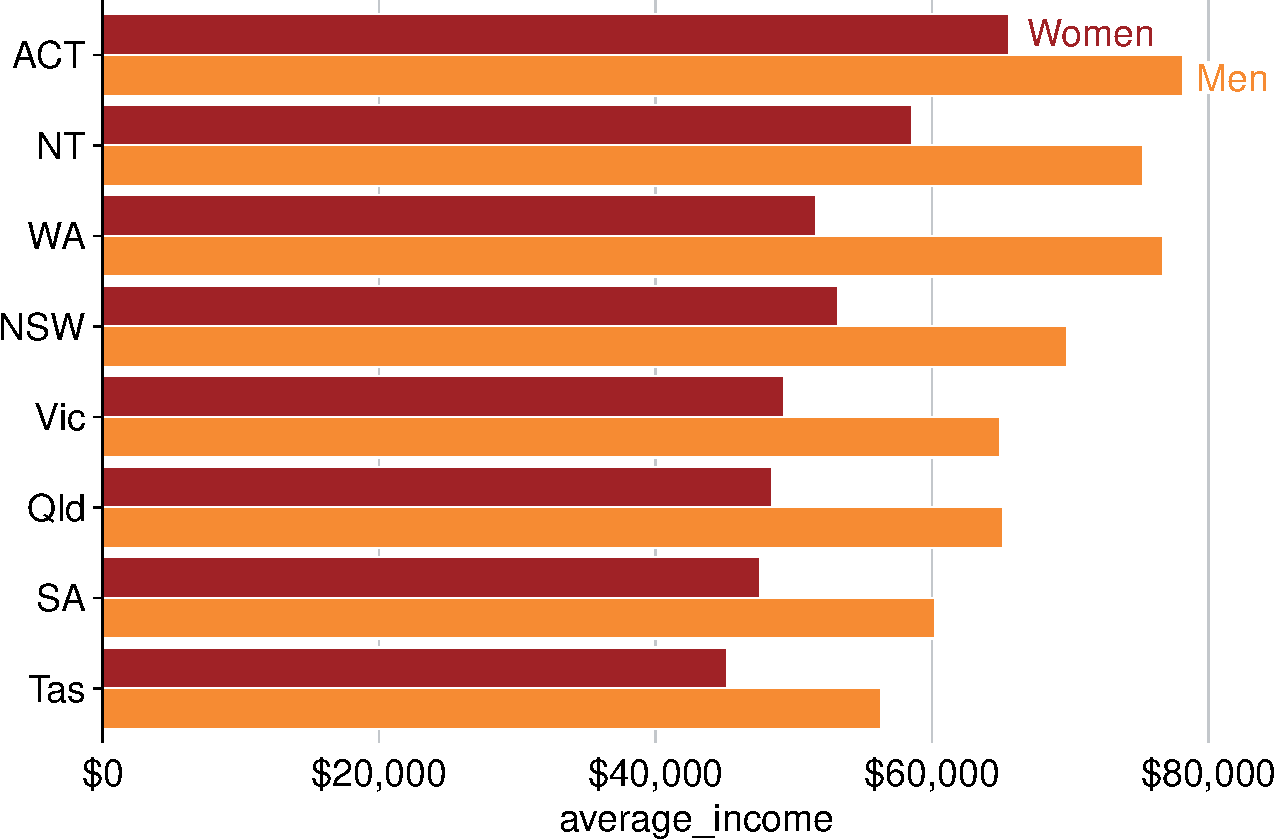
\includegraphics{Visualisation_cookbook_files/figure-latex/bar_multi_expand-1.pdf}

Looks magic! Now you can add titles and a caption, and save using \texttt{grattan\_save}:

\begin{Shaded}
\begin{Highlighting}[]
\NormalTok{multiple_bar <-}\StringTok{ }\NormalTok{data }\OperatorTok\StringTok{ }
\StringTok{  }\KeywordTok{ggplot}\NormalTok{(}\KeywordTok{aes}\NormalTok{(}\DataTypeTok{x =} \KeywordTok{reorder}\NormalTok{(state, average_income), }
             \DataTypeTok{y =}\NormalTok{ average_income,}
             \DataTypeTok{fill =}\NormalTok{ gender)) }\OperatorTok{+}\StringTok{ }
\StringTok{  }\KeywordTok{geom_col}\NormalTok{(}\DataTypeTok{position =} \StringTok{"dodge"}\NormalTok{) }\OperatorTok{+}\StringTok{ }
\StringTok{  }\KeywordTok{coord_flip}\NormalTok{() }\OperatorTok{+}\StringTok{ }
\StringTok{  }\KeywordTok{theme_grattan}\NormalTok{(}\DataTypeTok{flipped =} \OtherTok{TRUE}\NormalTok{) }\OperatorTok{+}\StringTok{ }
\StringTok{  }\KeywordTok{grattan_y_continuous}\NormalTok{(}\DataTypeTok{labels =}\NormalTok{ dollar, }
                       \DataTypeTok{expand_top =} \FloatTok{.1}\NormalTok{) }\OperatorTok{+}\StringTok{ }
\StringTok{  }\KeywordTok{grattan_fill_manual}\NormalTok{(}\DecValTok{2}\NormalTok{) }\OperatorTok{+}\StringTok{ }
\StringTok{  }\KeywordTok{grattan_label}\NormalTok{(}\DataTypeTok{data =}\NormalTok{ label_gender, }
                \KeywordTok{aes}\NormalTok{(}\DataTypeTok{colour =}\NormalTok{ gender,}
                    \DataTypeTok{label =}\NormalTok{ gender), }
                \DataTypeTok{position =} \KeywordTok{position_dodge}\NormalTok{(}\DataTypeTok{width =} \DecValTok{1}\NormalTok{), }
                \DataTypeTok{hjust =} \FloatTok{-0.1}\NormalTok{) }\OperatorTok{+}\StringTok{ }
\StringTok{  }\KeywordTok{grattan_colour_manual}\NormalTok{(}\DecValTok{2}\NormalTok{) }\OperatorTok{+}\StringTok{ }
\StringTok{  }\KeywordTok{labs}\NormalTok{(}\DataTypeTok{title =} \StringTok{"Women earn less than men in every state"}\NormalTok{,}
       \DataTypeTok{subtitle =} \StringTok{"Average income of workers, 2016"}\NormalTok{,}
       \DataTypeTok{x =} \StringTok{""}\NormalTok{,}
       \DataTypeTok{y =} \StringTok{""}\NormalTok{,}
       \DataTypeTok{caption =} \StringTok{"Notes: Only includes people who submitted a tax return in 2016-16. Source: ABS (2018)"}\NormalTok{)}
\end{Highlighting}
\end{Shaded}

\begin{Shaded}
\begin{Highlighting}[]
\KeywordTok{grattan_save}\NormalTok{(}\StringTok{"atlas/multiple_bar.pdf"}\NormalTok{, multiple_bar, }\DataTypeTok{type =} \StringTok{"fullslide"}\NormalTok{)}
\end{Highlighting}
\end{Shaded}

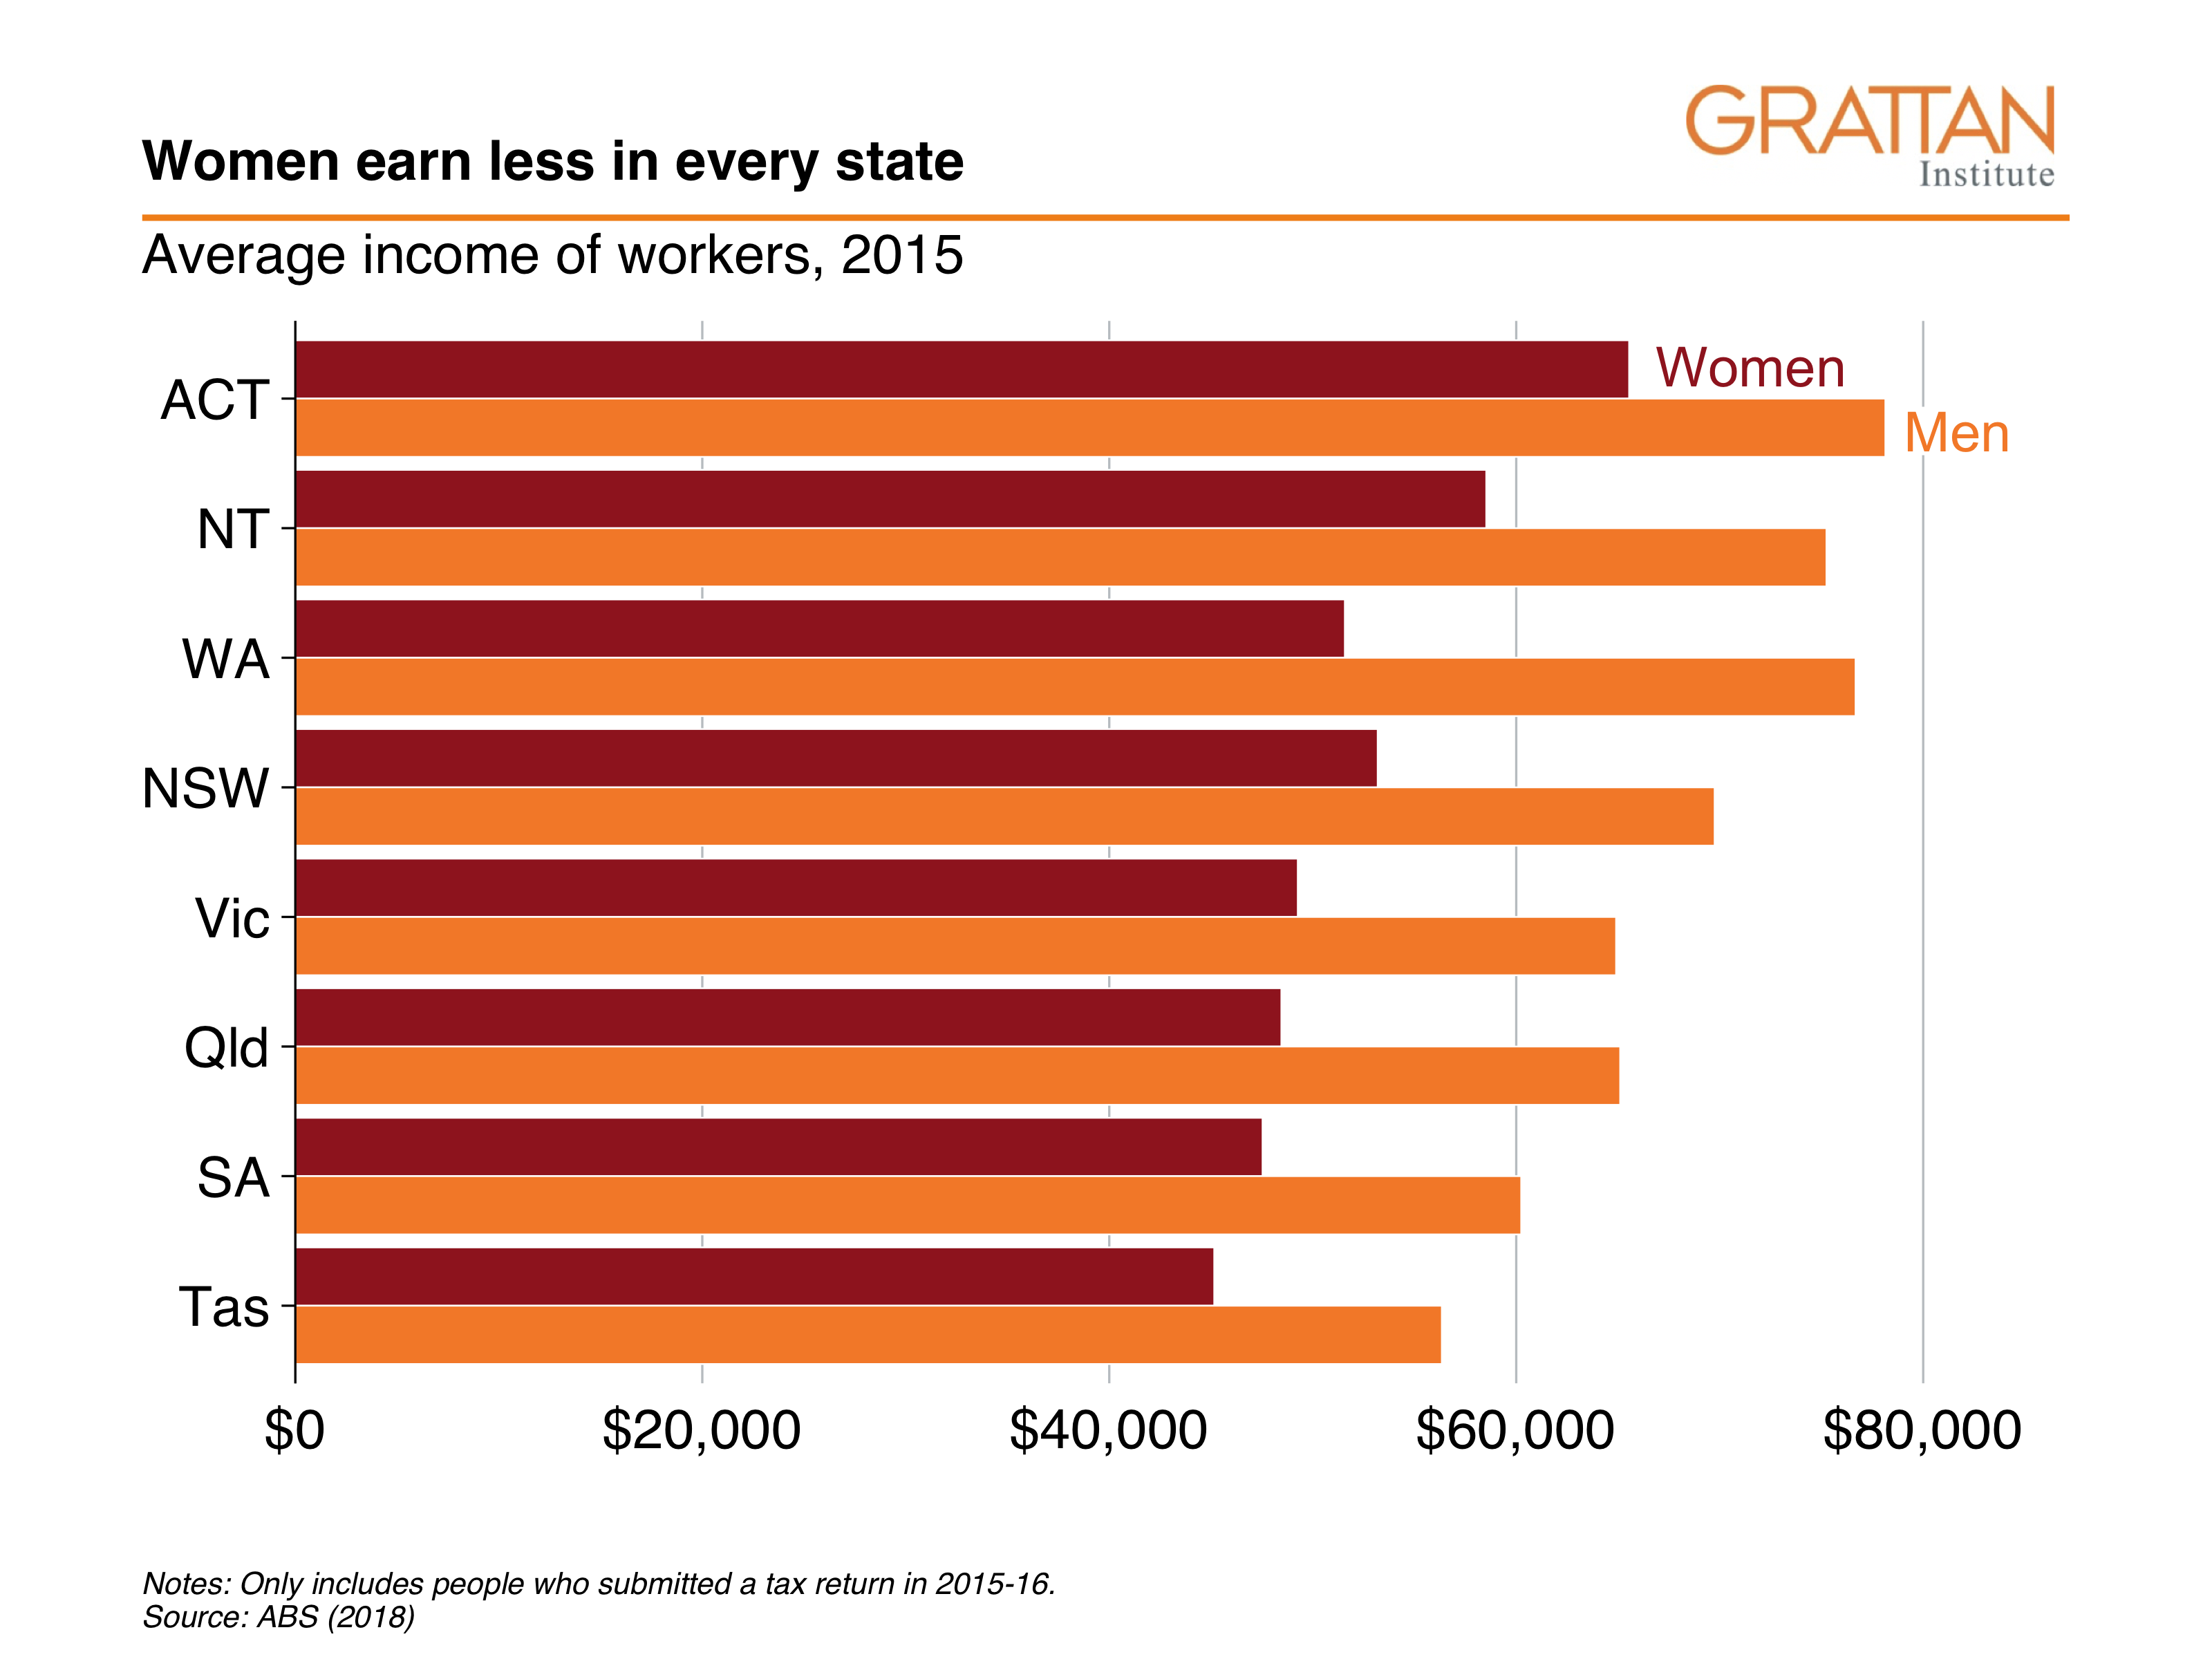
\includegraphics[width=44.44in]{atlas/multiple_bar}

\hypertarget{facet-bar}{%
\subsection{Facetted bar charts}\label{facet-bar}}

`Facetting' a chart means you create a separate plot for each group. It's particularly useful in showing differences between more than one group. The chart you'll make in this section will show annual income by gender and state, \emph{and} by professional and non-professional workers:

Start by creating the dataset you want to plot:

\begin{Shaded}
\begin{Highlighting}[]
\NormalTok{data <-}\StringTok{ }\NormalTok{sa3_income }\OperatorTok\StringTok{ }
\StringTok{  }\KeywordTok{group_by}\NormalTok{(state, gender, prof) }\OperatorTok\StringTok{ }
\StringTok{  }\KeywordTok{summarise}\NormalTok{(}\DataTypeTok{average_income =} \KeywordTok{sum}\NormalTok{(total_income) }\OperatorTok{/}\StringTok{ }\KeywordTok{sum}\NormalTok{(workers))}

\NormalTok{data}
\end{Highlighting}
\end{Shaded}

\begin{verbatim}
## # A tibble: 32 x 4
## # Groups:   state, gender [16]
##    state gender prof             average_income
##    <chr> <chr>  <chr>                     <dbl>
##  1 ACT   Men    Non-professional         52545.
##  2 ACT   Men    Professional             96488.
##  3 ACT   Women  Non-professional         46151.
##  4 ACT   Women  Professional             79828.
##  5 NSW   Men    Non-professional         49182.
##  6 NSW   Men    Professional             91624.
##  7 NSW   Women  Non-professional         36772.
##  8 NSW   Women  Professional             68445.
##  9 NT    Men    Non-professional         58844.
## 10 NT    Men    Professional             87666.
## # ... with 22 more rows
\end{verbatim}

Then plot a bar chart with \texttt{geom\_col} and \texttt{theme\_grattan} elements, using a similar chain to the final plot of \ref{bar-multi} (without the labelling). We'll build on this chart:

\begin{Shaded}
\begin{Highlighting}[]
\NormalTok{facet_bar <-}\StringTok{ }\NormalTok{data }\OperatorTok\StringTok{ }
\StringTok{  }\KeywordTok{ggplot}\NormalTok{(}\KeywordTok{aes}\NormalTok{(}\DataTypeTok{x =} \KeywordTok{reorder}\NormalTok{(state, average_income),}
             \DataTypeTok{y =}\NormalTok{ average_income,}
             \DataTypeTok{fill =}\NormalTok{ gender)) }\OperatorTok{+}\StringTok{ }
\StringTok{  }\KeywordTok{geom_col}\NormalTok{(}\DataTypeTok{position =} \StringTok{"dodge"}\NormalTok{) }\OperatorTok{+}\StringTok{ }
\StringTok{  }\KeywordTok{coord_flip}\NormalTok{() }\OperatorTok{+}\StringTok{ }
\StringTok{  }\KeywordTok{theme_grattan}\NormalTok{(}\DataTypeTok{flipped =} \OtherTok{TRUE}\NormalTok{) }\OperatorTok{+}\StringTok{ }
\StringTok{  }\KeywordTok{grattan_y_continuous}\NormalTok{(}\DataTypeTok{labels =}\NormalTok{ dollar, }
                       \DataTypeTok{expand_top =} \FloatTok{.1}\NormalTok{) }\OperatorTok{+}\StringTok{ }
\StringTok{  }\KeywordTok{grattan_fill_manual}\NormalTok{(}\DecValTok{2}\NormalTok{) }\OperatorTok{+}\StringTok{ }
\StringTok{  }\KeywordTok{grattan_colour_manual}\NormalTok{(}\DecValTok{2}\NormalTok{) }\OperatorTok{+}\StringTok{ }
\StringTok{  }\KeywordTok{labs}\NormalTok{(}\DataTypeTok{title =} \StringTok{"Professional workers earn more in every state"}\NormalTok{,}
       \DataTypeTok{subtitle =} \StringTok{"Average income of workers, 2016"}\NormalTok{,}
       \DataTypeTok{x =} \StringTok{""}\NormalTok{,}
       \DataTypeTok{y =} \StringTok{""}\NormalTok{,}
       \DataTypeTok{caption =} \StringTok{"Notes: Only includes people who submitted a tax return in 2016-16. Source: ABS (2018)"}\NormalTok{)}
\end{Highlighting}
\end{Shaded}

You can `facet' bar charts -- and any other chart type -- with the \texttt{facet\_grid} or \texttt{facet\_wrap} commands. The latter tends to give you more control over label placement, so let's start with that. \texttt{fadcet\_wrap} asks the questions: ``what variables should I create separete charts for'', and ``how should I place them on the page''? Tell it to use the \texttt{prof} variable with the \texttt{vars()} function.\footnote{The \texttt{vars()} function is sometimes used in the \texttt{tidyverse} to specifically say ``I am using a variable name here''. You can't use variable names directly because of legacy issues. You can learn more about it in the \href{https://ggplot2.tidyverse.org/reference/facet_wrap.html}{official documentation}.}

\begin{Shaded}
\begin{Highlighting}[]
\NormalTok{facet_bar }\OperatorTok{+}
\StringTok{  }\KeywordTok{facet_wrap}\NormalTok{(}\KeywordTok{vars}\NormalTok{(prof))}
\end{Highlighting}
\end{Shaded}

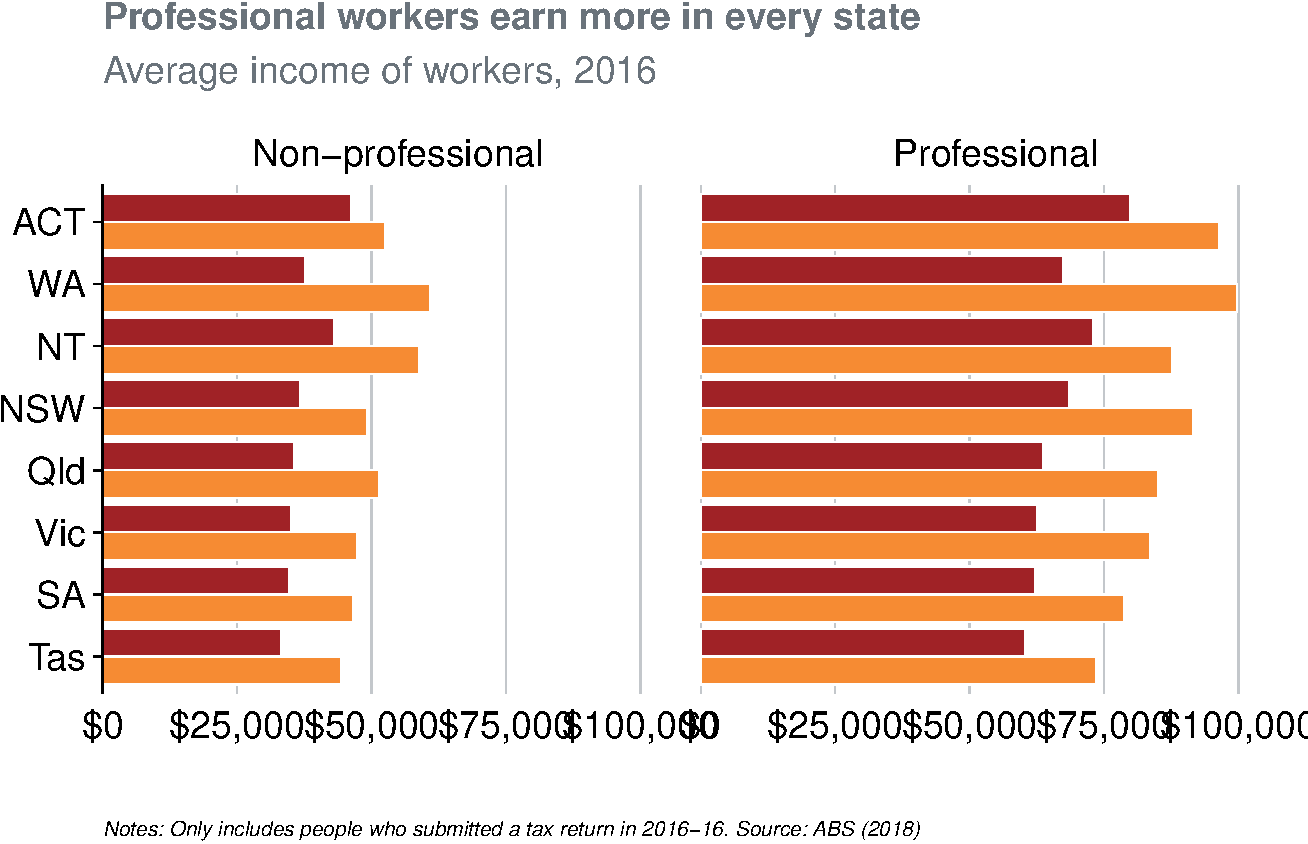
\includegraphics{Visualisation_cookbook_files/figure-latex/bar_facet_wrap-1.pdf}

That's good! It does what it should. Now you just need to tidy it up a little bit by adding labels and avoiding clashes along the bottom axis.

Create labels in the same way you have done before: you only want to label one `women' and `men' series, so create a dataset that contains only that information:

\begin{Shaded}
\begin{Highlighting}[]
\NormalTok{label_data <-}\StringTok{ }\NormalTok{data }\OperatorTok\StringTok{ }
\StringTok{  }\KeywordTok{filter}\NormalTok{(state }\OperatorTok{==}\StringTok{ "ACT"}\NormalTok{,}
\NormalTok{         prof }\OperatorTok{==}\StringTok{ "Non-professional"}\NormalTok{)}

\NormalTok{label_data}
\end{Highlighting}
\end{Shaded}

\begin{verbatim}
## # A tibble: 2 x 4
## # Groups:   state, gender [2]
##   state gender prof             average_income
##   <chr> <chr>  <chr>                     <dbl>
## 1 ACT   Men    Non-professional         52545.
## 2 ACT   Women  Non-professional         46151.
\end{verbatim}

Good -- now add that to the plot with \texttt{grattan\_label}, supplying the required aesthetics and position. And use \texttt{hjust\ =\ 0} to tell the labels to be left-aligned.

To give each plot a black base axis, you can add \texttt{geom\_hline()} with \texttt{yintercept\ =\ 0}.

\begin{Shaded}
\begin{Highlighting}[]
\NormalTok{facet_bar }\OperatorTok{+}
\StringTok{  }\KeywordTok{facet_wrap}\NormalTok{(}\KeywordTok{vars}\NormalTok{(prof)) }\OperatorTok{+}\StringTok{ }
\StringTok{  }\KeywordTok{geom_hline}\NormalTok{(}\DataTypeTok{yintercept =} \DecValTok{0}\NormalTok{) }\OperatorTok{+}\StringTok{  }\CommentTok{# add black line}
\StringTok{  }\KeywordTok{grattan_label}\NormalTok{(}\DataTypeTok{data =}\NormalTok{ label_data, }\CommentTok{# supply label data}
                \KeywordTok{aes}\NormalTok{(}\DataTypeTok{label =}\NormalTok{ gender,}
                    \DataTypeTok{colour =}\NormalTok{ gender),}
                \DataTypeTok{position =} \KeywordTok{position_dodge}\NormalTok{(}\DataTypeTok{width =} \DecValTok{1}\NormalTok{), }
                \DataTypeTok{hjust =} \DecValTok{0}\NormalTok{)}
\end{Highlighting}
\end{Shaded}

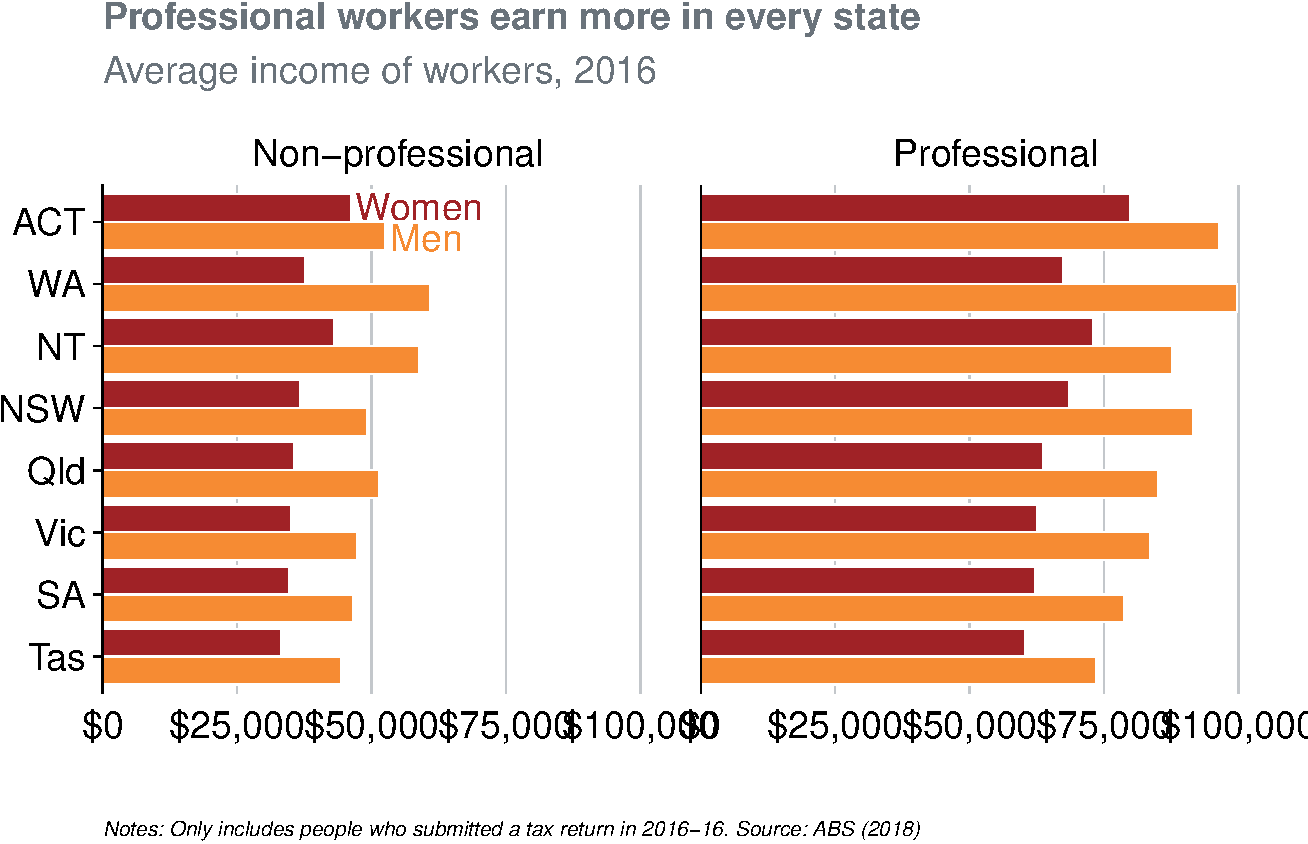
\includegraphics{Visualisation_cookbook_files/figure-latex/bar_facet_label-1.pdf}

Wicked! But the ``\$0'' and ``\$100,000'' labels are clashing along the horizontal axis. To tidy these up, we redefine the \texttt{breaks} -- the points that will be labelled -- to 25,000, 50,000 and 75,000 inside \texttt{grattan\_y\_continuous}. Putting everything together and saving the plot as a fullslide chart with \texttt{grattan\_save}:

\begin{Shaded}
\begin{Highlighting}[]
\CommentTok{# Create label data}
\NormalTok{label_data <-}\StringTok{ }\NormalTok{data }\OperatorTok\StringTok{ }
\StringTok{  }\KeywordTok{filter}\NormalTok{(state }\OperatorTok{==}\StringTok{ "ACT"}\NormalTok{,}
\NormalTok{         prof }\OperatorTok{==}\StringTok{ "Non-professional"}\NormalTok{)}

\CommentTok{# Create plot}
\NormalTok{facet_bar <-}\StringTok{ }\NormalTok{data }\OperatorTok\StringTok{ }
\StringTok{  }\KeywordTok{ggplot}\NormalTok{(}\KeywordTok{aes}\NormalTok{(}\DataTypeTok{x =} \KeywordTok{reorder}\NormalTok{(state, average_income),}
             \DataTypeTok{y =}\NormalTok{ average_income,}
             \DataTypeTok{fill =}\NormalTok{ gender)) }\OperatorTok{+}\StringTok{ }
\StringTok{  }\KeywordTok{geom_col}\NormalTok{(}\DataTypeTok{position =} \StringTok{"dodge"}\NormalTok{) }\OperatorTok{+}\StringTok{ }
\StringTok{  }\KeywordTok{coord_flip}\NormalTok{() }\OperatorTok{+}\StringTok{ }
\StringTok{  }\KeywordTok{theme_grattan}\NormalTok{(}\DataTypeTok{flipped =} \OtherTok{TRUE}\NormalTok{) }\OperatorTok{+}\StringTok{ }
\StringTok{  }\KeywordTok{grattan_y_continuous}\NormalTok{(}\DataTypeTok{labels =}\NormalTok{ dollar,}
                       \DataTypeTok{breaks =} \KeywordTok{c}\NormalTok{(}\FloatTok{25e3}\NormalTok{, }\FloatTok{50e3}\NormalTok{, }\FloatTok{75e3}\NormalTok{)) }\OperatorTok{+}\StringTok{  }\CommentTok{# change breaks}
\StringTok{  }\KeywordTok{grattan_fill_manual}\NormalTok{(}\DecValTok{2}\NormalTok{) }\OperatorTok{+}\StringTok{ }
\StringTok{  }\KeywordTok{grattan_colour_manual}\NormalTok{(}\DecValTok{2}\NormalTok{) }\OperatorTok{+}\StringTok{ }
\StringTok{  }\KeywordTok{labs}\NormalTok{(}\DataTypeTok{title =} \StringTok{"Professional workers earn more in every state"}\NormalTok{,}
       \DataTypeTok{subtitle =} \StringTok{"Average income of workers, 2016"}\NormalTok{,}
       \DataTypeTok{x =} \StringTok{""}\NormalTok{,}
       \DataTypeTok{y =} \StringTok{""}\NormalTok{,}
       \DataTypeTok{caption =} \StringTok{"Notes: Only includes people who submitted a tax return in 2016-16. Source: ABS (2018)"}\NormalTok{) }\OperatorTok{+}\StringTok{ }
\StringTok{  }\KeywordTok{facet_wrap}\NormalTok{(}\KeywordTok{vars}\NormalTok{(prof)) }\OperatorTok{+}\StringTok{ }
\StringTok{  }\KeywordTok{grattan_label}\NormalTok{(}\DataTypeTok{data =}\NormalTok{ label_data,}
                \KeywordTok{aes}\NormalTok{(}\DataTypeTok{label =}\NormalTok{ gender,}
                    \DataTypeTok{colour =}\NormalTok{ gender),}
                \DataTypeTok{position =} \KeywordTok{position_dodge}\NormalTok{(}\DataTypeTok{width =} \DecValTok{1}\NormalTok{), }
                \DataTypeTok{hjust =} \DecValTok{0}\NormalTok{)}
\end{Highlighting}
\end{Shaded}

\begin{Shaded}
\begin{Highlighting}[]
\KeywordTok{grattan_save}\NormalTok{(}\StringTok{"atlas/facet_bar.pdf"}\NormalTok{, facet_bar, }\DataTypeTok{type =} \StringTok{"fullslide"}\NormalTok{)}
\end{Highlighting}
\end{Shaded}

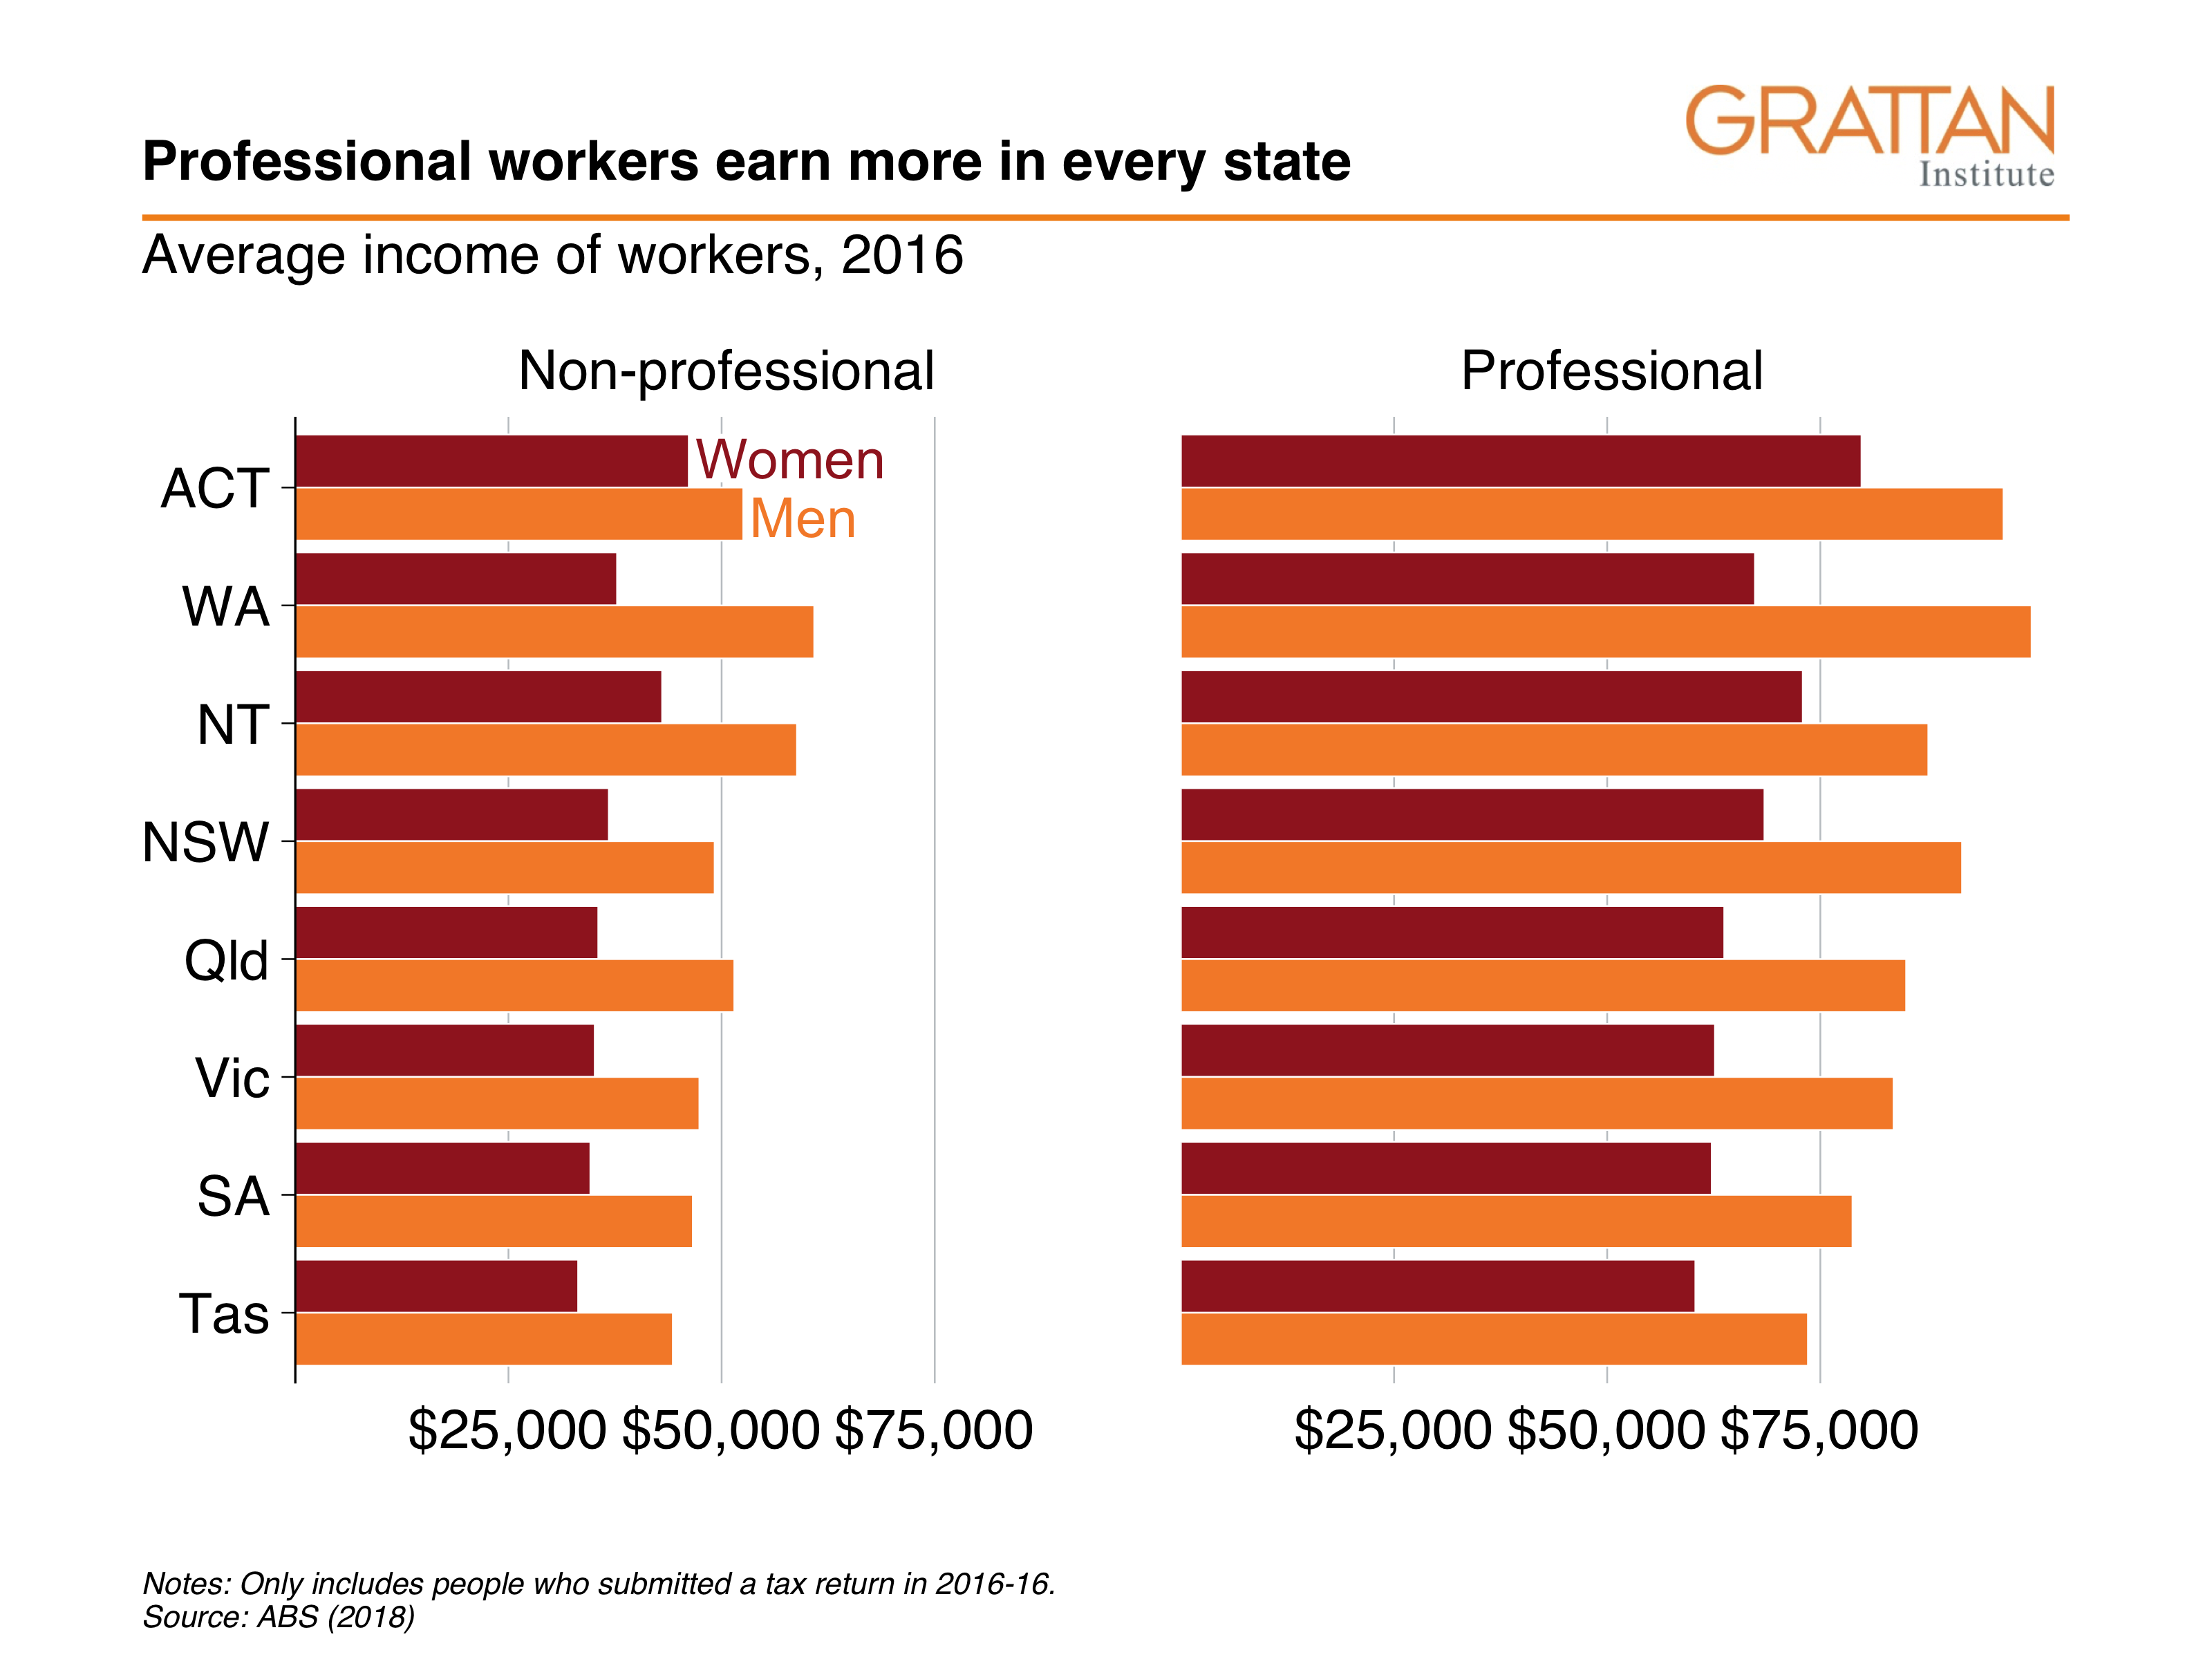
\includegraphics[width=44.44in]{atlas/facet_bar}

\hypertarget{line-charts}{%
\section{Line charts}\label{line-charts}}

A line chart has one key aesthetic: \texttt{group}. This tells \texttt{ggplot} how to connect individual lines.

\hypertarget{simple-line-chart}{%
\subsection{Simple line chart}\label{simple-line-chart}}

The first line chart shows the number of workers in Australia between 2011 and 2016:

\hypertarget{line-chart-with-multiple-series}{%
\subsection{Line chart with multiple series}\label{line-chart-with-multiple-series}}

This line chart will show how \textbf{real} average income has changed for each state over the past five years:

First, take the \texttt{sa3\_income} dataset and create a summary table average income by year and state. Ignore the territories for this chart.

\begin{Shaded}
\begin{Highlighting}[]
\NormalTok{data <-}\StringTok{ }\NormalTok{sa3_income }\OperatorTok\StringTok{ }
\StringTok{  }\KeywordTok{filter}\NormalTok{(}\OperatorTok{!}\NormalTok{state }\OperatorTok\StringTok{ }\KeywordTok{c}\NormalTok{(}\StringTok{"ACT"}\NormalTok{, }\StringTok{"NT"}\NormalTok{)) }\OperatorTok\StringTok{ }
\StringTok{  }\KeywordTok{group_by}\NormalTok{(year, state) }\OperatorTok\StringTok{ }
\StringTok{  }\KeywordTok{summarise}\NormalTok{(}\DataTypeTok{average_income =} \KeywordTok{sum}\NormalTok{(total_income) }\OperatorTok{/}\StringTok{ }\KeywordTok{sum}\NormalTok{(workers))}

\KeywordTok{head}\NormalTok{(data)}
\end{Highlighting}
\end{Shaded}

\begin{verbatim}
## # A tibble: 6 x 3
## # Groups:   year [1]
##    year state average_income
##   <dbl> <chr>          <dbl>
## 1  2011 NSW           55483.
## 2  2011 Qld           51408.
## 3  2011 SA            48443.
## 4  2011 Tas           45439.
## 5  2011 Vic           52053.
## 6  2011 WA            58795.
\end{verbatim}

The income data presented is nominal, so you'll need to inflate to `real' dollars using the `cpi\_inflate

Plot a line chart by taking the \texttt{data}, passing it to \texttt{ggplot} with \emph{aes}thetics, then using \texttt{geom\_line}:

\begin{Shaded}
\begin{Highlighting}[]
\NormalTok{data }\OperatorTok\StringTok{ }
\StringTok{  }\KeywordTok{ggplot}\NormalTok{(}\KeywordTok{aes}\NormalTok{(}\DataTypeTok{x =}\NormalTok{ year,}
             \DataTypeTok{y =}\NormalTok{ average_income,}
             \DataTypeTok{group =}\NormalTok{ state)) }\OperatorTok{+}\StringTok{ }
\StringTok{  }\KeywordTok{geom_line}\NormalTok{()}
\end{Highlighting}
\end{Shaded}

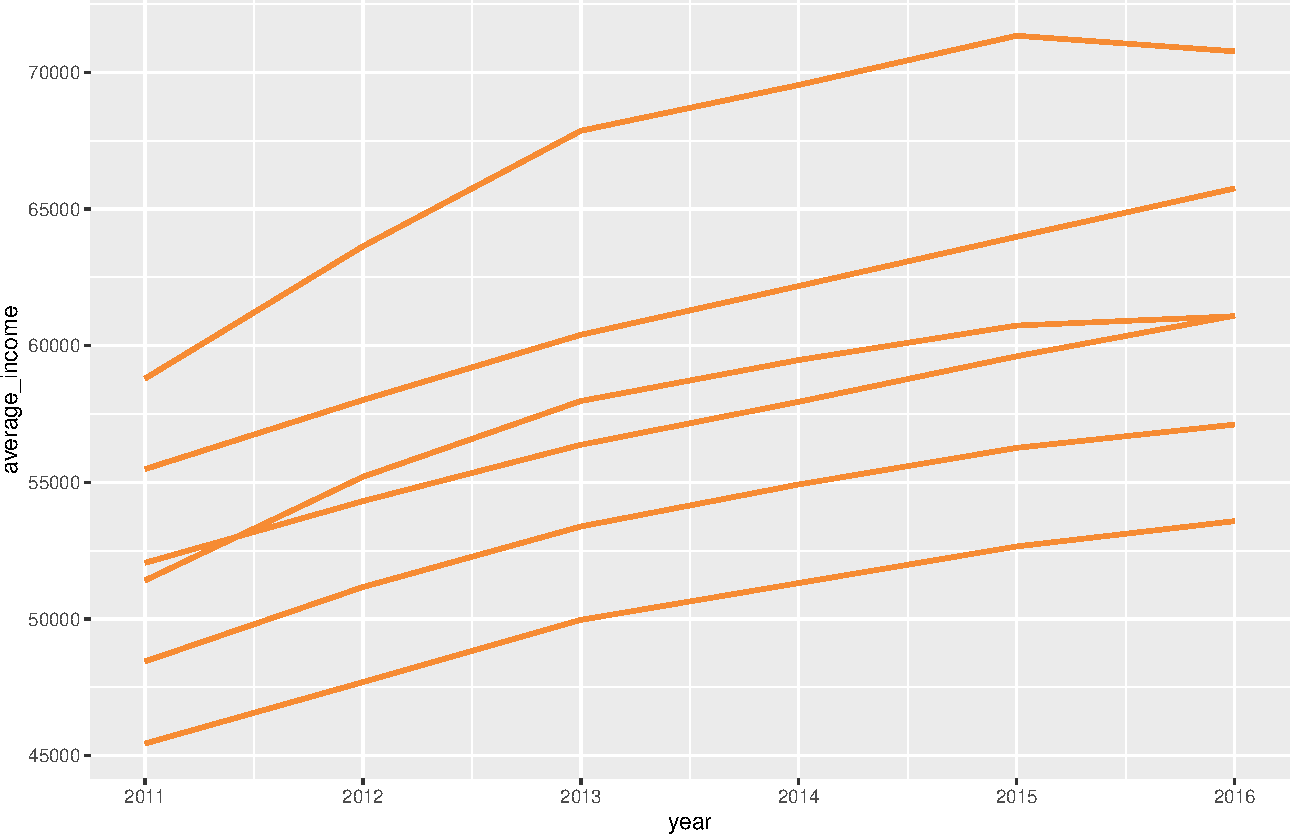
\includegraphics{Visualisation_cookbook_files/figure-latex/line1_nocol-1.pdf}

Now you can represent each \texttt{state} by colour:

\begin{Shaded}
\begin{Highlighting}[]
\NormalTok{data }\OperatorTok\StringTok{ }
\StringTok{  }\KeywordTok{ggplot}\NormalTok{(}\KeywordTok{aes}\NormalTok{(}\DataTypeTok{x =}\NormalTok{ year,}
             \DataTypeTok{y =}\NormalTok{ average_income,}
             \DataTypeTok{group =}\NormalTok{ state,}
             \DataTypeTok{colour =}\NormalTok{ state)) }\OperatorTok{+}\StringTok{ }
\StringTok{  }\KeywordTok{geom_line}\NormalTok{()}
\end{Highlighting}
\end{Shaded}

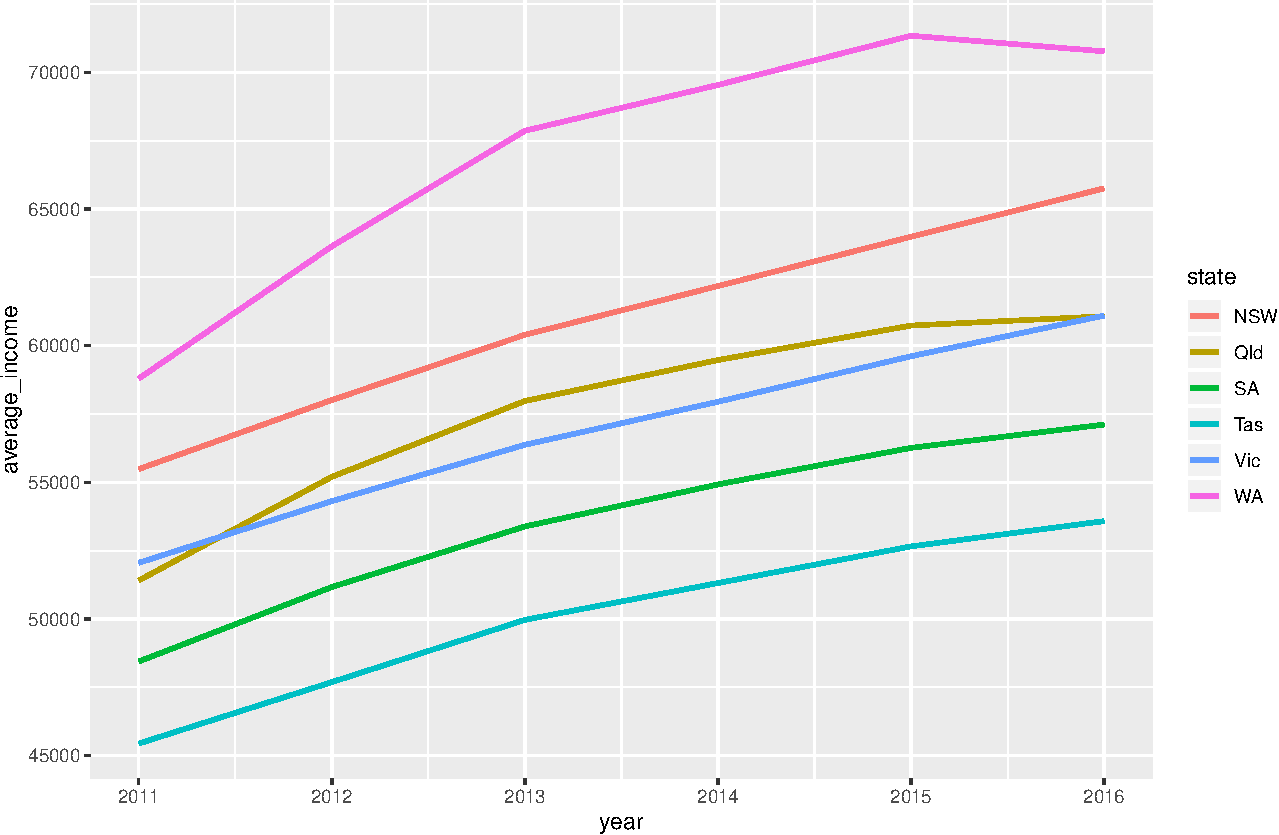
\includegraphics{Visualisation_cookbook_files/figure-latex/line1_wcol-1.pdf}

Cooler! Adding some Grattan formatting to it and define it as our `base chart':

\begin{Shaded}
\begin{Highlighting}[]
\NormalTok{base_chart <-data }\OperatorTok\StringTok{ }
\StringTok{  }\KeywordTok{ggplot}\NormalTok{(}\KeywordTok{aes}\NormalTok{(}\DataTypeTok{x =}\NormalTok{ year,}
             \DataTypeTok{y =}\NormalTok{ average_income,}
             \DataTypeTok{group =}\NormalTok{ state,}
             \DataTypeTok{colour =}\NormalTok{ state)) }\OperatorTok{+}\StringTok{ }
\StringTok{  }\KeywordTok{geom_line}\NormalTok{() }\OperatorTok{+}
\StringTok{  }\KeywordTok{theme_grattan}\NormalTok{() }\OperatorTok{+}\StringTok{ }
\StringTok{  }\KeywordTok{grattan_y_continuous}\NormalTok{(}\DataTypeTok{labels =}\NormalTok{ comma) }\OperatorTok{+}\StringTok{ }
\StringTok{  }\KeywordTok{grattan_colour_manual}\NormalTok{(}\DecValTok{6}\NormalTok{) }\OperatorTok{+}
\StringTok{  }\KeywordTok{labs}\NormalTok{(}\DataTypeTok{x =} \StringTok{""}\NormalTok{,}
       \DataTypeTok{y =} \StringTok{""}\NormalTok{)}

\NormalTok{base_chart}
\end{Highlighting}
\end{Shaded}

\includegraphics{Visualisation_cookbook_files/figure-latex/unnamed-chunk-2-1.pdf}

You can add `dots' for each year by layering \texttt{geom\_point} on top of \texttt{geom\_line}:

\begin{Shaded}
\begin{Highlighting}[]
\NormalTok{base_chart }\OperatorTok{+}
\StringTok{  }\KeywordTok{geom_point}\NormalTok{()}
\end{Highlighting}
\end{Shaded}

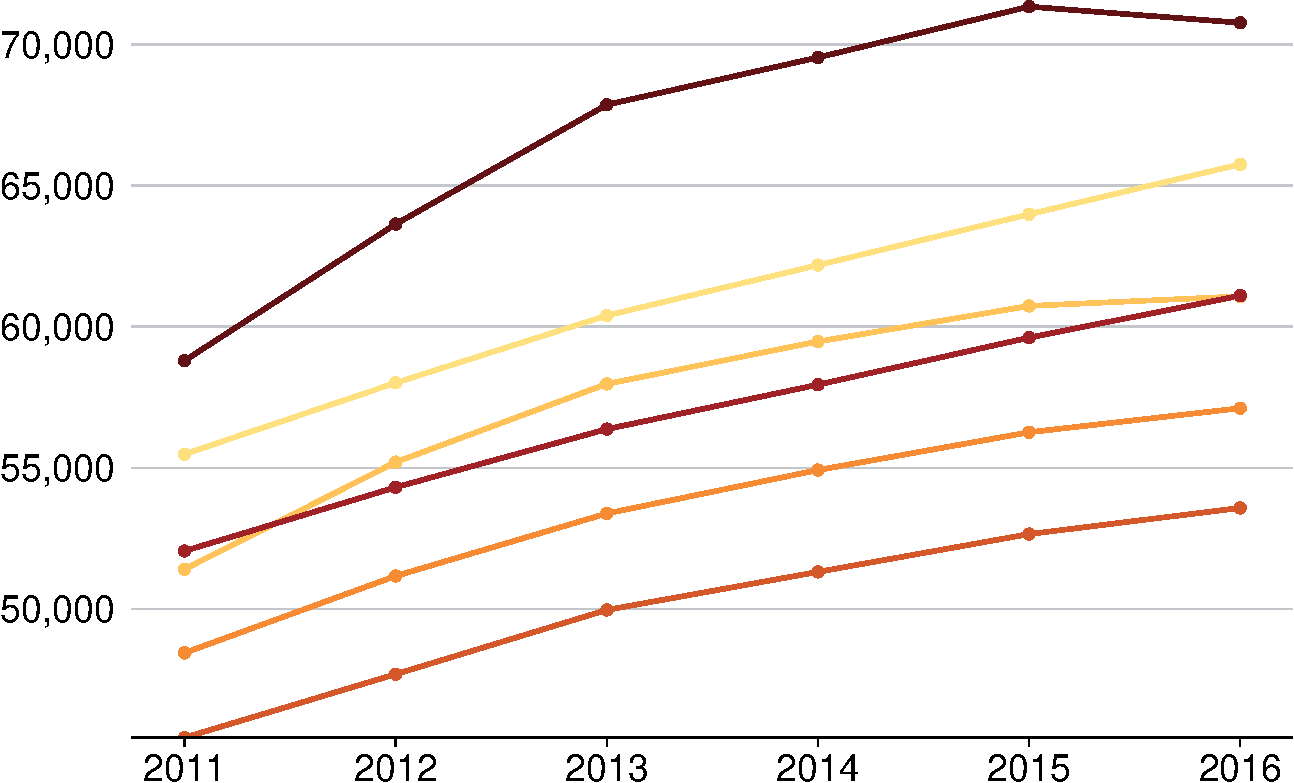
\includegraphics{Visualisation_cookbook_files/figure-latex/line2-1.pdf}

To add labels to the end of each line, you would expand the x-axis to make room for labels and add reasonable breaks:

\begin{Shaded}
\begin{Highlighting}[]
\NormalTok{base_chart }\OperatorTok{+}
\StringTok{  }\KeywordTok{grattan_x_continuous}\NormalTok{(}\DataTypeTok{expand_right =} \FloatTok{.3}\NormalTok{,}
                       \DataTypeTok{breaks =} \KeywordTok{seq}\NormalTok{(}\DecValTok{2011}\NormalTok{, }\DecValTok{2016}\NormalTok{, }\DecValTok{1}\NormalTok{),}
                       \DataTypeTok{labels =} \KeywordTok{c}\NormalTok{(}\StringTok{"2011"}\NormalTok{, }\StringTok{"12"}\NormalTok{, }\StringTok{"13"}\NormalTok{, }\StringTok{"14"}\NormalTok{, }\StringTok{"15"}\NormalTok{, }\StringTok{"16"}\NormalTok{)) }
\end{Highlighting}
\end{Shaded}

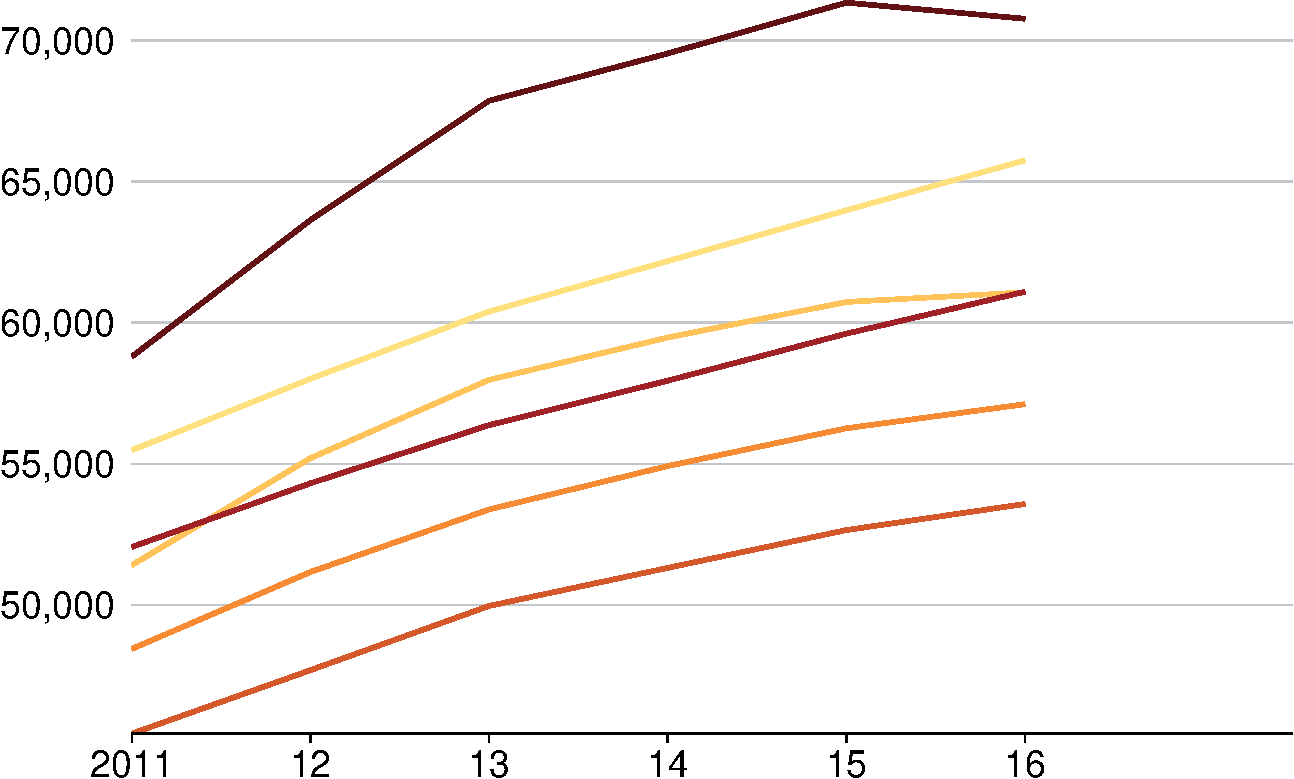
\includegraphics{Visualisation_cookbook_files/figure-latex/line_expand-1.pdf}

Then add labels, using

\begin{Shaded}
\begin{Highlighting}[]
\NormalTok{label_line <-}\StringTok{ }\NormalTok{data }\OperatorTok\StringTok{ }
\StringTok{  }\KeywordTok{filter}\NormalTok{(year }\OperatorTok{==}\StringTok{ }\DecValTok{2010}\NormalTok{)}

\NormalTok{base_chart }\OperatorTok{+}
\StringTok{  }\KeywordTok{geom_point}\NormalTok{() }\OperatorTok{+}
\StringTok{  }\KeywordTok{grattan_x_continuous}\NormalTok{(}\DataTypeTok{expand_left =} \FloatTok{.1}\NormalTok{,}
                       \DataTypeTok{breaks =} \KeywordTok{seq}\NormalTok{(}\DecValTok{2011}\NormalTok{, }\DecValTok{2016}\NormalTok{, }\DecValTok{1}\NormalTok{),}
                       \DataTypeTok{labels =} \KeywordTok{c}\NormalTok{(}\StringTok{"2011"}\NormalTok{, }\StringTok{"12"}\NormalTok{, }\StringTok{"13"}\NormalTok{, }\StringTok{"14"}\NormalTok{, }\StringTok{"15"}\NormalTok{, }\StringTok{"16"}\NormalTok{)) }\OperatorTok{+}\StringTok{ }
\StringTok{  }\KeywordTok{grattan_label}\NormalTok{(}\DataTypeTok{data =}\NormalTok{ label_line,}
                \KeywordTok{aes}\NormalTok{(}\DataTypeTok{label =}\NormalTok{ state),}
                \DataTypeTok{nudge_x =} \OperatorTok{-}\OtherTok{Inf}\NormalTok{,}
                \DataTypeTok{segment.colour =} \OtherTok{NA}\NormalTok{)}
\end{Highlighting}
\end{Shaded}

\begin{verbatim}
## Warning: Ignoring unknown parameters: segment.colour
\end{verbatim}

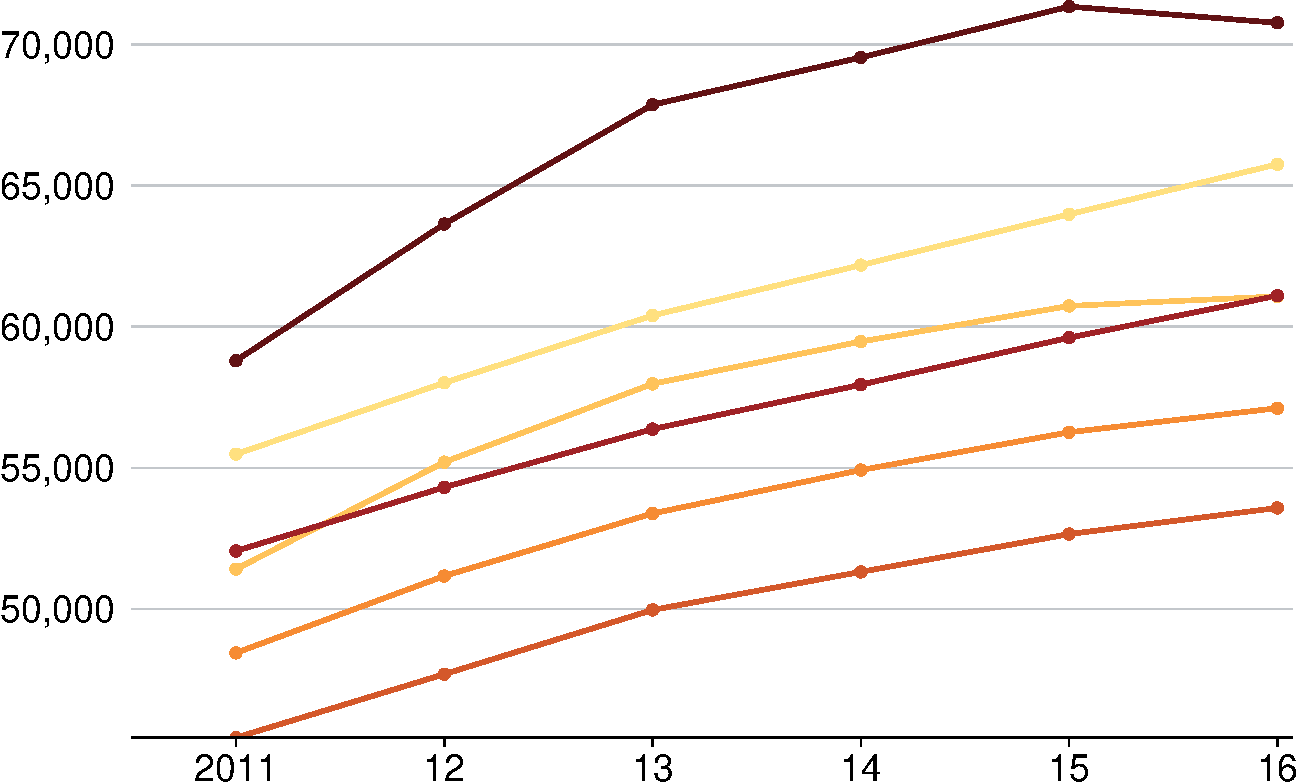
\includegraphics{Visualisation_cookbook_files/figure-latex/line_label-1.pdf}
If you wanted to show each state individually, you could \textbf{facet} your chart so that a separate plot was produced for each state:

\begin{Shaded}
\begin{Highlighting}[]
\NormalTok{base_chart }\OperatorTok{+}
\StringTok{  }\KeywordTok{geom_point}\NormalTok{() }\OperatorTok{+}
\StringTok{    }\KeywordTok{grattan_x_continuous}\NormalTok{(}\DataTypeTok{expand_left =} \FloatTok{.1}\NormalTok{, }
                         \DataTypeTok{expand_right =} \FloatTok{.1}\NormalTok{,}
                         \DataTypeTok{breaks =} \KeywordTok{seq}\NormalTok{(}\DecValTok{2011}\NormalTok{, }\DecValTok{2016}\NormalTok{, }\DecValTok{1}\NormalTok{),}
                         \DataTypeTok{labels =} \KeywordTok{c}\NormalTok{(}\StringTok{"2011"}\NormalTok{, }\StringTok{"12"}\NormalTok{, }\StringTok{"13"}\NormalTok{, }\StringTok{"14"}\NormalTok{, }\StringTok{"15"}\NormalTok{, }\StringTok{"16"}\NormalTok{)) }\OperatorTok{+}\StringTok{ }
\StringTok{  }\KeywordTok{theme}\NormalTok{(}\DataTypeTok{panel.spacing.x =} \KeywordTok{unit}\NormalTok{(}\DecValTok{10}\NormalTok{, }\StringTok{"mm"}\NormalTok{)) }\OperatorTok{+}\StringTok{ }
\StringTok{  }\KeywordTok{facet_wrap}\NormalTok{(state }\OperatorTok{~}\StringTok{ }\NormalTok{.)}
\end{Highlighting}
\end{Shaded}

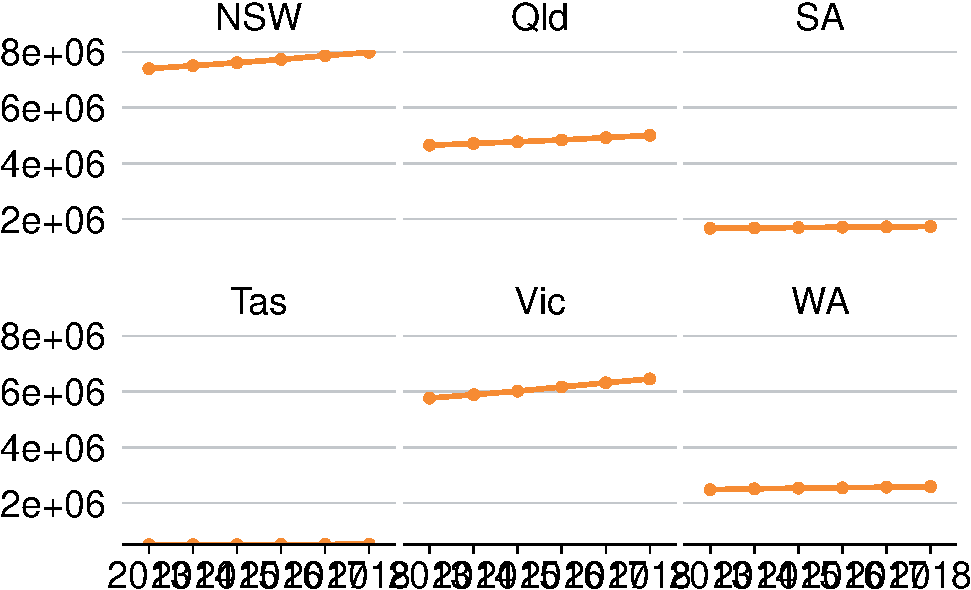
\includegraphics{Visualisation_cookbook_files/figure-latex/line3-1.pdf}

\hypertarget{scatter-plots}{%
\section{Scatter plots}\label{scatter-plots}}

Scatter plots require \texttt{x} and \texttt{y} aesthetics. These can then be coloured and faceted.

\hypertarget{simple-scatter-plot}{%
\subsection{Simple scatter plot}\label{simple-scatter-plot}}

The first simple scatter plot will show the relationship between average incomes of professionals and the number of professional workers by area in 2016:

\begin{Shaded}
\begin{Highlighting}[]
\KeywordTok{include_graphics}\NormalTok{(}\StringTok{"atlas/simple_scatter.png"}\NormalTok{)}
\end{Highlighting}
\end{Shaded}

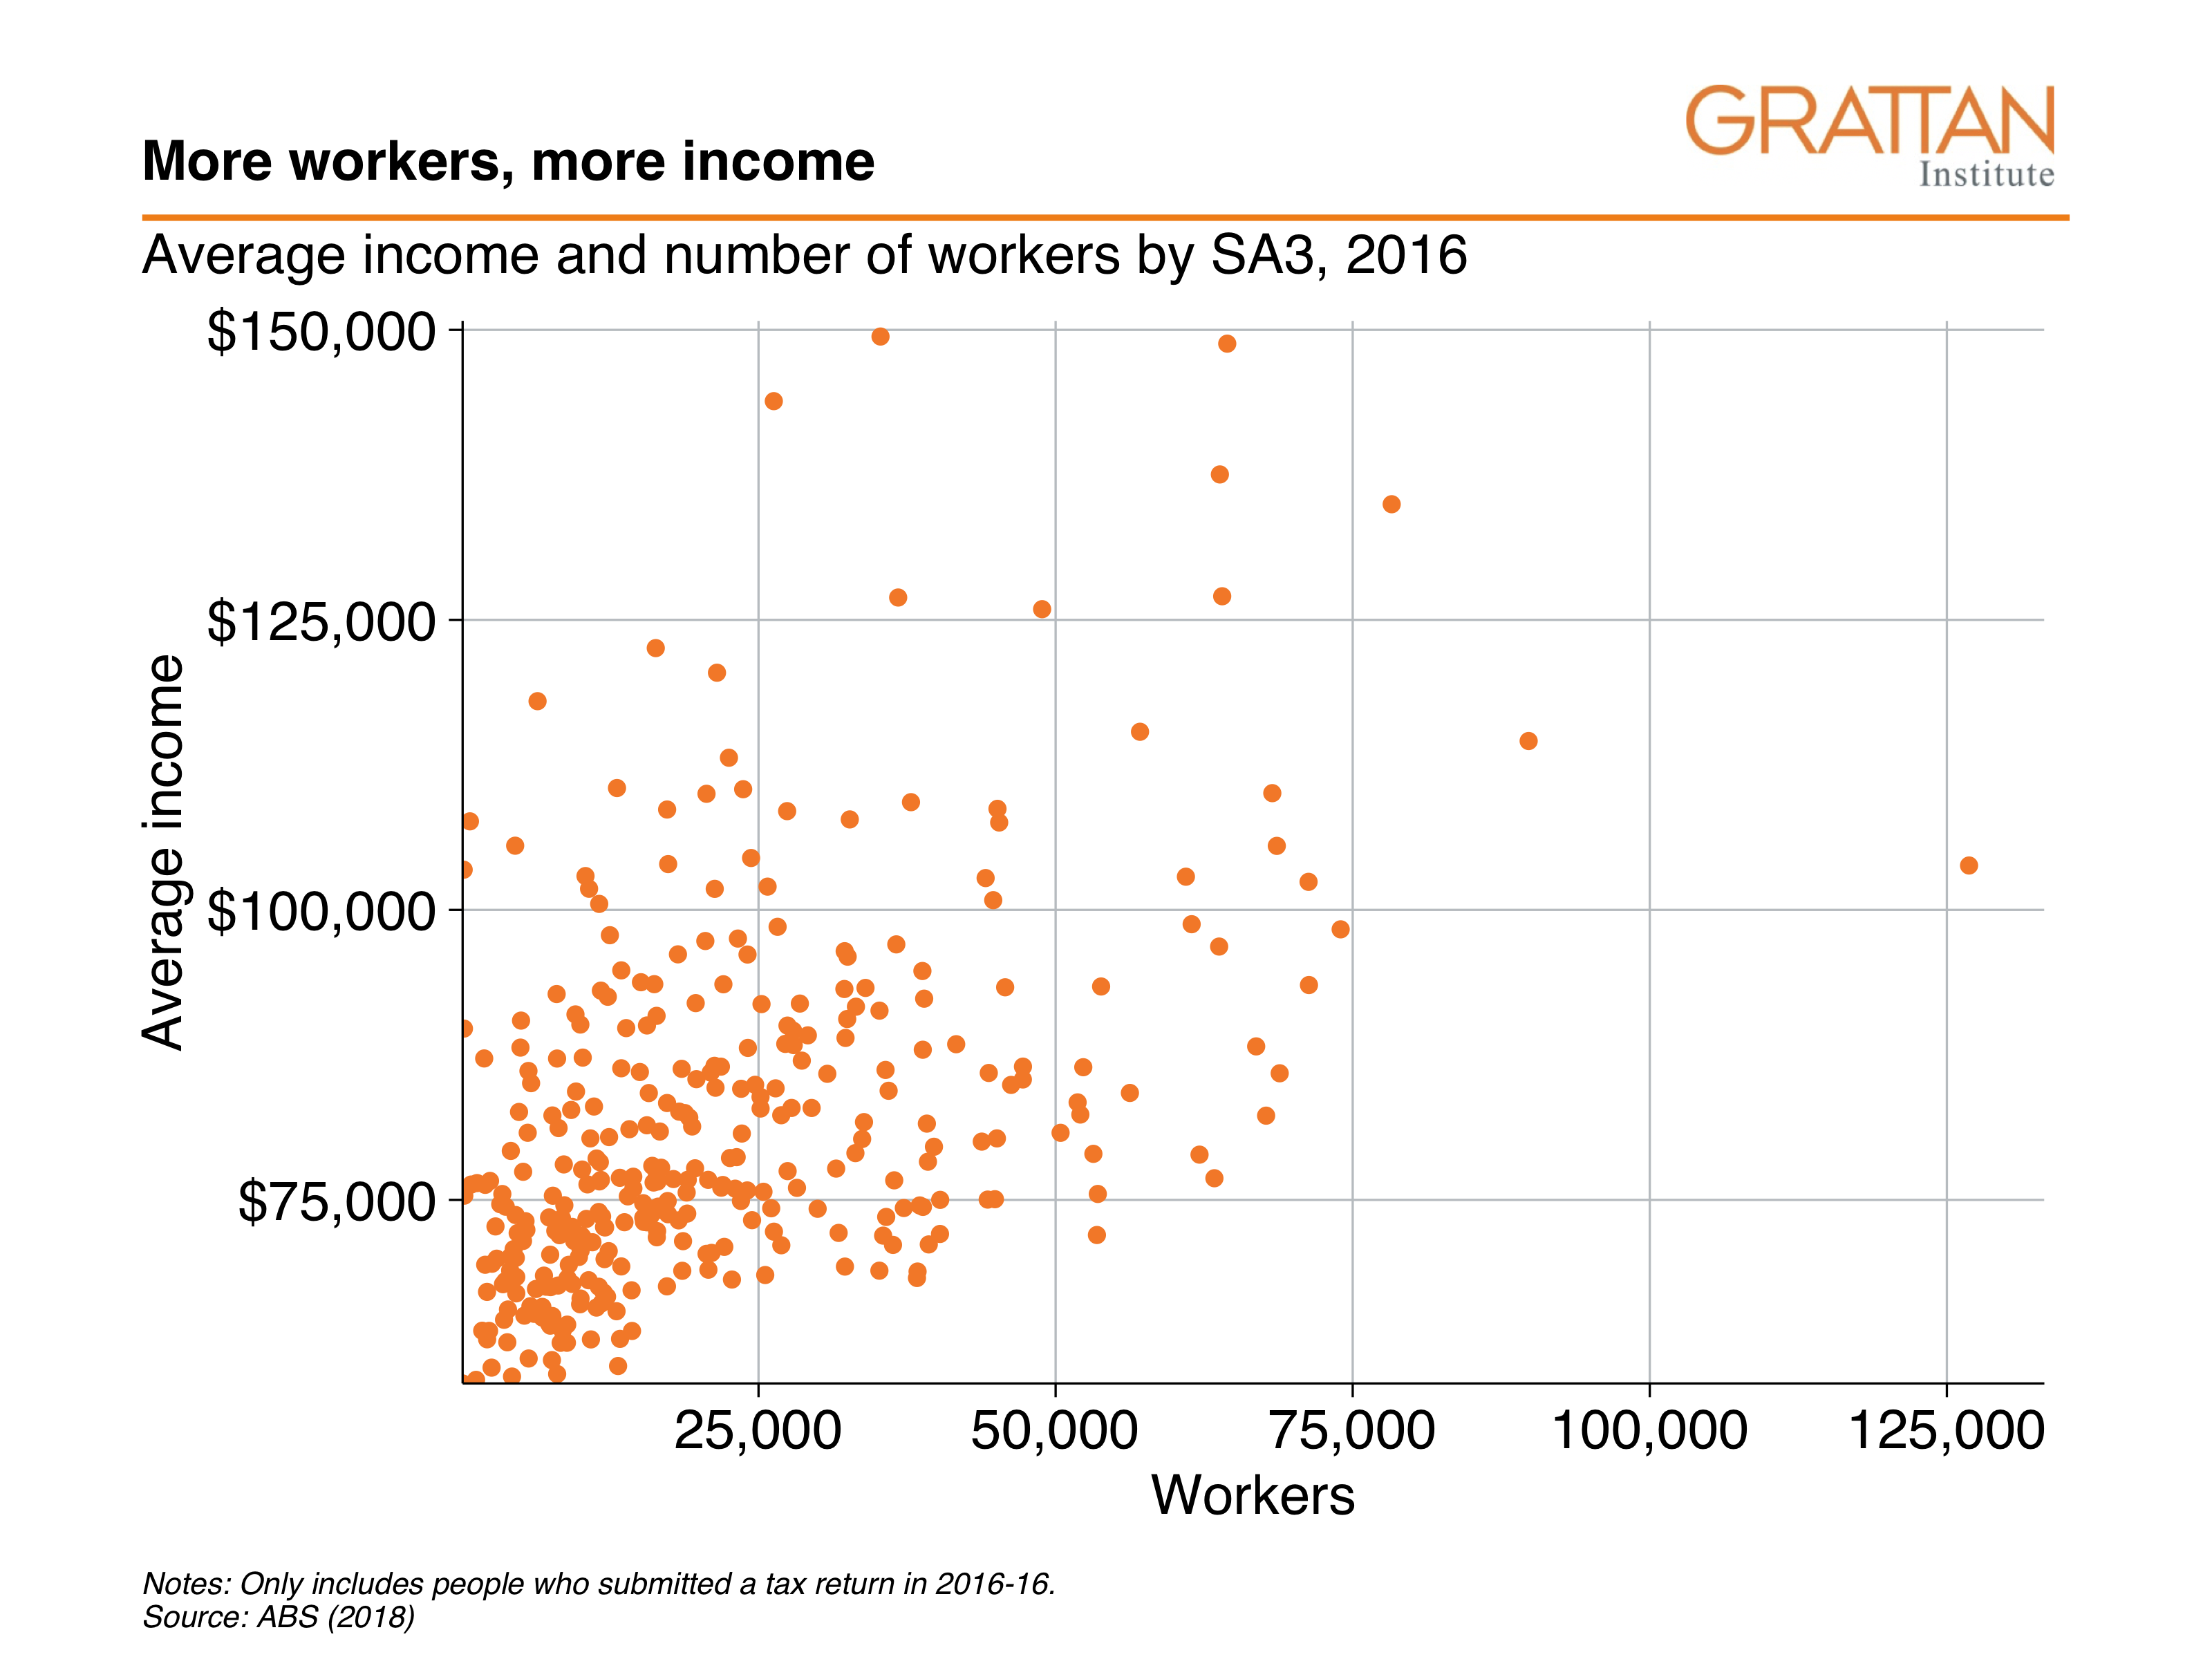
\includegraphics[width=44.44in]{atlas/simple_scatter}

Create the dataset you want to plot:

\begin{Shaded}
\begin{Highlighting}[]
\NormalTok{data <-}\StringTok{ }\NormalTok{sa3_income }\OperatorTok\StringTok{ }
\StringTok{  }\KeywordTok{filter}\NormalTok{(year }\OperatorTok{==}\StringTok{ }\DecValTok{2016}\NormalTok{,}
\NormalTok{         prof }\OperatorTok{==}\StringTok{ "Professional"}\NormalTok{) }\OperatorTok\StringTok{ }
\StringTok{  }\KeywordTok{group_by}\NormalTok{(sa3_name) }\OperatorTok\StringTok{ }
\StringTok{  }\KeywordTok{summarise}\NormalTok{(}\DataTypeTok{workers =} \KeywordTok{sum}\NormalTok{(workers),}
            \DataTypeTok{average_income =} \KeywordTok{sum}\NormalTok{(total_income) }\OperatorTok{/}\StringTok{ }\NormalTok{workers)}

\KeywordTok{head}\NormalTok{(data)}
\end{Highlighting}
\end{Shaded}

\begin{verbatim}
## # A tibble: 6 x 3
##   sa3_name       workers average_income
##   <chr>            <dbl>          <dbl>
## 1 Adelaide City    10005         90115.
## 2 Adelaide Hills   24715         84921.
## 3 Albany           12390         70581.
## 4 Albury           16465         72305.
## 5 Alice Springs     9640         84340.
## 6 Armadale         19771         85407.
\end{verbatim}

The dataset has one observation per SA3, and the two variables you want to plot: workers and average income. Pass the data to \texttt{ggplot}, set the aesthetics and plot with \texttt{geom\_point}:

\begin{Shaded}
\begin{Highlighting}[]
\NormalTok{data }\OperatorTok\StringTok{ }
\StringTok{  }\KeywordTok{ggplot}\NormalTok{(}\KeywordTok{aes}\NormalTok{(}\DataTypeTok{x =}\NormalTok{ workers,}
             \DataTypeTok{y =}\NormalTok{ average_income)) }\OperatorTok{+}\StringTok{ }
\StringTok{  }\KeywordTok{geom_point}\NormalTok{()}
\end{Highlighting}
\end{Shaded}

\includegraphics{Visualisation_cookbook_files/figure-latex/simple_scatter_base-1.pdf}

Then add Grattan theme elements:

\begin{itemize}
\tightlist
\item
  \texttt{theme\_grattan()}, telling it that the \texttt{chart\_type} is a scatter plot.
\item
  \texttt{grattan\_y\_continuous()}, setting the label style to \texttt{dollar}.
\item
  \texttt{grattan\_x\_continuous()}, setting the label style to \texttt{comma}.
\end{itemize}

\begin{Shaded}
\begin{Highlighting}[]
\NormalTok{data }\OperatorTok\StringTok{ }
\StringTok{  }\KeywordTok{ggplot}\NormalTok{(}\KeywordTok{aes}\NormalTok{(}\DataTypeTok{x =}\NormalTok{ workers,}
             \DataTypeTok{y =}\NormalTok{ average_income)) }\OperatorTok{+}\StringTok{ }
\StringTok{  }\KeywordTok{geom_point}\NormalTok{()  }\OperatorTok{+}
\StringTok{  }\KeywordTok{theme_grattan}\NormalTok{(}\DataTypeTok{chart_type =} \StringTok{"scatter"}\NormalTok{) }\OperatorTok{+}\StringTok{ }
\StringTok{  }\KeywordTok{grattan_y_continuous}\NormalTok{(}\DataTypeTok{labels =}\NormalTok{ dollar) }\OperatorTok{+}\StringTok{ }
\StringTok{  }\KeywordTok{grattan_x_continuous}\NormalTok{(}\DataTypeTok{labels =}\NormalTok{ comma)}
\end{Highlighting}
\end{Shaded}

\includegraphics{Visualisation_cookbook_files/figure-latex/simple_scatter_grattan-1.pdf}

Looks brilliant. The last label on the x-axis goes off the page a bit so you can expand the plot to the right in the \texttt{grattan\_x\_continuous} element:

\begin{Shaded}
\begin{Highlighting}[]
\NormalTok{data }\OperatorTok\StringTok{ }
\StringTok{  }\KeywordTok{ggplot}\NormalTok{(}\KeywordTok{aes}\NormalTok{(}\DataTypeTok{x =}\NormalTok{ workers,}
             \DataTypeTok{y =}\NormalTok{ average_income)) }\OperatorTok{+}\StringTok{ }
\StringTok{  }\KeywordTok{geom_point}\NormalTok{()  }\OperatorTok{+}
\StringTok{  }\KeywordTok{theme_grattan}\NormalTok{(}\DataTypeTok{chart_type =} \StringTok{"scatter"}\NormalTok{) }\OperatorTok{+}\StringTok{ }
\StringTok{  }\KeywordTok{grattan_y_continuous}\NormalTok{(}\DataTypeTok{labels =}\NormalTok{ dollar) }\OperatorTok{+}\StringTok{ }
\StringTok{  }\KeywordTok{grattan_x_continuous}\NormalTok{(}\DataTypeTok{labels =}\NormalTok{ comma,}
                       \DataTypeTok{expand_right =} \FloatTok{.05}\NormalTok{) }\CommentTok{# expand the right by 5%}
\end{Highlighting}
\end{Shaded}

\includegraphics{Visualisation_cookbook_files/figure-latex/simple_scatter_expand-1.pdf}

Finally, add titles and save the plot:

\begin{Shaded}
\begin{Highlighting}[]
\NormalTok{simple_scatter <-}\StringTok{ }\NormalTok{data }\OperatorTok\StringTok{ }
\StringTok{  }\KeywordTok{ggplot}\NormalTok{(}\KeywordTok{aes}\NormalTok{(}\DataTypeTok{x =}\NormalTok{ workers,}
             \DataTypeTok{y =}\NormalTok{ average_income)) }\OperatorTok{+}\StringTok{ }
\StringTok{  }\KeywordTok{geom_point}\NormalTok{()  }\OperatorTok{+}
\StringTok{  }\KeywordTok{theme_grattan}\NormalTok{(}\DataTypeTok{chart_type =} \StringTok{"scatter"}\NormalTok{) }\OperatorTok{+}\StringTok{ }
\StringTok{  }\KeywordTok{grattan_y_continuous}\NormalTok{(}\DataTypeTok{labels =}\NormalTok{ dollar) }\OperatorTok{+}\StringTok{ }
\StringTok{  }\KeywordTok{grattan_x_continuous}\NormalTok{(}\DataTypeTok{labels =}\NormalTok{ comma,}
                       \DataTypeTok{expand_right =} \FloatTok{.05}\NormalTok{) }\OperatorTok{+}\StringTok{ }
\StringTok{  }\KeywordTok{labs}\NormalTok{(}\DataTypeTok{title =} \StringTok{"More workers, more income"}\NormalTok{,}
       \DataTypeTok{subtitle =} \StringTok{"Average income and number of workers by SA3, 2016"}\NormalTok{,}
       \DataTypeTok{y =} \StringTok{"Average income"}\NormalTok{,}
       \DataTypeTok{x =} \StringTok{"Workers"}\NormalTok{,}
       \DataTypeTok{caption =} \StringTok{"Notes: Only includes people who submitted a tax return in 2016-16. Source: ABS (2018)"}\NormalTok{)}
\end{Highlighting}
\end{Shaded}

\begin{Shaded}
\begin{Highlighting}[]
\KeywordTok{grattan_save}\NormalTok{(}\StringTok{"atlas/simple_scatter.pdf"}\NormalTok{, simple_scatter, }\DataTypeTok{type =} \StringTok{"fullslide"}\NormalTok{)}
\end{Highlighting}
\end{Shaded}

\includegraphics[width=44.44in]{atlas/simple_scatter}

\hypertarget{scatter-plot-with-reshaped-data}{%
\subsection{Scatter plot with reshaped data}\label{scatter-plot-with-reshaped-data}}

The next scatter plot involves the same basic plotting principles of the chart above, but requires a bit more data manipulation before plotting.

The chart will show the wages of professional workers and non-professional workers in 2016:

\begin{Shaded}
\begin{Highlighting}[]
\KeywordTok{include_graphics}\NormalTok{(}\StringTok{"atlas/scatter_reshape.png"}\NormalTok{)}
\end{Highlighting}
\end{Shaded}

\includegraphics[width=44.44in]{atlas/scatter_reshape}

First prepare your data. You want to find the average incomes of all professional and non-professional workers in 2016:

\begin{Shaded}
\begin{Highlighting}[]
\NormalTok{data_prep <-}\StringTok{ }\NormalTok{sa3_income }\OperatorTok\StringTok{ }
\StringTok{  }\KeywordTok{filter}\NormalTok{(year }\OperatorTok{==}\StringTok{ }\DecValTok{2016}\NormalTok{) }\OperatorTok\StringTok{ }
\StringTok{  }\KeywordTok{group_by}\NormalTok{(sa3_name, prof) }\OperatorTok\StringTok{ }
\StringTok{  }\KeywordTok{summarise}\NormalTok{(}\DataTypeTok{average_income =} \KeywordTok{sum}\NormalTok{(total_income) }\OperatorTok{/}\StringTok{ }\KeywordTok{sum}\NormalTok{(workers))}

\KeywordTok{head}\NormalTok{(data_prep)}
\end{Highlighting}
\end{Shaded}

\begin{verbatim}
## # A tibble: 6 x 3
## # Groups:   sa3_name [3]
##   sa3_name       prof             average_income
##   <chr>          <chr>                     <dbl>
## 1 Adelaide City  Non-professional         40843.
## 2 Adelaide City  Professional             90115.
## 3 Adelaide Hills Non-professional         47208.
## 4 Adelaide Hills Professional             84921.
## 5 Albany         Non-professional         46609.
## 6 Albany         Professional             70581.
\end{verbatim}

That's good -- you have the numbers you need. But think about how you're going to \emph{plot} them using \texttt{x} and \texttt{y} aesthetics. You'll need one variable for \texttt{x\ =\ professional\_income} and one variable for \texttt{y\ =\ non\_professional\_income}. At the moment, these are represented by different \emph{rows}.

You can fix this by reshaping the data with the \texttt{pivot\_wider} function. The three arguments you provide here are:

\begin{itemize}
\tightlist
\item
  \texttt{id\_cols\ =\ sa3\_name}: the variable \texttt{sa3\_name} uniquely identifies each row in your data.
\item
  \texttt{names\_from\ =\ prof}: the variable \texttt{prof} contains the variables names for the \emph{new} variables you are creating.
\item
  \texttt{values\_from\ =\ average\_income}: the variable \texttt{average\_income} contains the \emph{values} that will fill the new variables.
\end{itemize}

After the \texttt{pivot\_wider} step is complete, use \texttt{janitor::clean\_names()} to convert the new \texttt{Professional} and \texttt{Non-Professional} names to \texttt{snake\_case} to make them easier to use down the track:

\begin{Shaded}
\begin{Highlighting}[]
\NormalTok{data <-}\StringTok{ }\NormalTok{data_prep }\OperatorTok\StringTok{ }
\StringTok{  }\KeywordTok{pivot_wider}\NormalTok{(}\DataTypeTok{id_cols =}\NormalTok{ sa3_name,  }\CommentTok{# variables that will stay the same}
              \DataTypeTok{names_from =}\NormalTok{ prof,   }\CommentTok{# variables that will dictate the new names}
              \DataTypeTok{values_from =}\NormalTok{ average_income) }\OperatorTok\StringTok{  }\CommentTok{# these will be the values}
\StringTok{  }\NormalTok{janitor}\OperatorTok{::}\KeywordTok{clean_names}\NormalTok{() }\CommentTok{# tidy up the new variable names}

\KeywordTok{head}\NormalTok{(data)}
\end{Highlighting}
\end{Shaded}

\begin{verbatim}
## # A tibble: 6 x 3
## # Groups:   sa3_name [6]
##   sa3_name       non_professional professional
##   <chr>                     <dbl>        <dbl>
## 1 Adelaide City            40843.       90115.
## 2 Adelaide Hills           47208.       84921.
## 3 Albany                   46609.       70581.
## 4 Albury                   44718.       72305.
## 5 Alice Springs            54647.       84340.
## 6 Armadale                 57599.       85407.
\end{verbatim}

Getting the data in the right format for your plot -- rather than `hacking' your plot to fit your data -- will save you time and effort down the line.

Now you have a dataset in the format you want to plot, you can pass it to \texttt{ggplot} and add aesthetics like you normally would.

\begin{Shaded}
\begin{Highlighting}[]
\NormalTok{data }\OperatorTok\StringTok{ }
\StringTok{  }\KeywordTok{ggplot}\NormalTok{(}\KeywordTok{aes}\NormalTok{(}\DataTypeTok{x =}\NormalTok{ non_professional,}
             \DataTypeTok{y =}\NormalTok{ professional)) }\OperatorTok{+}\StringTok{ }
\StringTok{  }\KeywordTok{geom_point}\NormalTok{(}\DataTypeTok{alpha =} \FloatTok{0.8}\NormalTok{) }\CommentTok{# make the points a little transparent}
\end{Highlighting}
\end{Shaded}

\begin{verbatim}
## Warning: Removed 1 rows containing missing values (geom_point).
\end{verbatim}

\includegraphics{Visualisation_cookbook_files/figure-latex/scatter_reshape_base-1.pdf}

Then, like you've done before, add Grattan theme elements and titles, and save with \texttt{grattan\_save}:

\begin{Shaded}
\begin{Highlighting}[]
\NormalTok{scatter_reshape <-}\StringTok{ }\NormalTok{data }\OperatorTok\StringTok{ }
\StringTok{  }\KeywordTok{ggplot}\NormalTok{(}\KeywordTok{aes}\NormalTok{(}\DataTypeTok{x =}\NormalTok{ non_professional,}
             \DataTypeTok{y =}\NormalTok{ professional)) }\OperatorTok{+}\StringTok{ }
\StringTok{  }\KeywordTok{geom_point}\NormalTok{(}\DataTypeTok{alpha =} \FloatTok{0.8}\NormalTok{) }\OperatorTok{+}\StringTok{ }
\StringTok{  }\KeywordTok{theme_grattan}\NormalTok{(}\DataTypeTok{chart_type =} \StringTok{"scatter"}\NormalTok{) }\OperatorTok{+}\StringTok{ }
\StringTok{  }\KeywordTok{grattan_y_continuous}\NormalTok{(}\DataTypeTok{labels =}\NormalTok{ dollar) }\OperatorTok{+}\StringTok{ }
\StringTok{  }\KeywordTok{grattan_x_continuous}\NormalTok{(}\DataTypeTok{labels =}\NormalTok{ dollar) }\OperatorTok{+}
\StringTok{  }\KeywordTok{labs}\NormalTok{(}\DataTypeTok{title =} \StringTok{"Non-professionals tend to earn more when professionals do"}\NormalTok{,}
       \DataTypeTok{subtitle =} \StringTok{"Average income for workers by SA3, 2016"}\NormalTok{,}
       \DataTypeTok{y =} \StringTok{"Professional incomes"}\NormalTok{,}
       \DataTypeTok{x =} \StringTok{"Non-professional incomes"}\NormalTok{,}
       \DataTypeTok{caption =} \StringTok{"Notes: Only includes people who submitted a tax return in 2016-16. Source: ABS (2018)"}\NormalTok{)}
\end{Highlighting}
\end{Shaded}

\begin{Shaded}
\begin{Highlighting}[]
\KeywordTok{grattan_save}\NormalTok{(}\StringTok{"atlas/scatter_reshape.pdf"}\NormalTok{, scatter_reshape, }\DataTypeTok{type =} \StringTok{"fullslide"}\NormalTok{)}
\end{Highlighting}
\end{Shaded}

\includegraphics[width=44.44in]{atlas/scatter_reshape}

\hypertarget{layered-scatter-plot}{%
\subsection{Layered scatter plot}\label{layered-scatter-plot}}

For the third plot, look at the incomes of non-professional workers by their area's total income percentile:

\begin{Shaded}
\begin{Highlighting}[]
\KeywordTok{include_graphics}\NormalTok{(}\StringTok{"atlas/scatter_layer.png"}\NormalTok{)}
\end{Highlighting}
\end{Shaded}

\includegraphics[width=44.44in]{atlas/scatter_layer}

Get the data you want to plot:

\begin{Shaded}
\begin{Highlighting}[]
\NormalTok{data <-}\StringTok{ }\NormalTok{sa3_income }\OperatorTok\StringTok{ }
\StringTok{  }\KeywordTok{filter}\NormalTok{(year }\OperatorTok{==}\StringTok{ }\DecValTok{2016}\NormalTok{) }\OperatorTok
\StringTok{  }\KeywordTok{mutate}\NormalTok{(}\DataTypeTok{total_income =}\NormalTok{ average_income }\OperatorTok{*}\StringTok{ }\NormalTok{workers) }\OperatorTok\StringTok{ }
\StringTok{  }\KeywordTok{group_by}\NormalTok{(sa3_name, sa3_income_percentile, prof, occ_short) }\OperatorTok\StringTok{ }
\StringTok{  }\KeywordTok{summarise}\NormalTok{(}\DataTypeTok{income =} \KeywordTok{sum}\NormalTok{(total_income),}
            \DataTypeTok{workers =} \KeywordTok{sum}\NormalTok{(workers),}
            \DataTypeTok{average_income =}\NormalTok{ income }\OperatorTok{/}\StringTok{ }\NormalTok{workers)}

\KeywordTok{head}\NormalTok{(data)}
\end{Highlighting}
\end{Shaded}

\begin{verbatim}
## # A tibble: 6 x 7
## # Groups:   sa3_name, sa3_income_percentile, prof [1]
##   sa3_name  sa3_income_perce~ prof  occ_short income workers average_income
##   <chr>                 <dbl> <chr> <chr>      <dbl>   <dbl>          <dbl>
## 1 Adelaide~                66 Non-~ Admin     1.44e8    2674         53979.
## 2 Adelaide~                66 Non-~ Driver    1.85e7     396         46762.
## 3 Adelaide~                66 Non-~ Labourer  3.92e7    1516         25868.
## 4 Adelaide~                66 Non-~ Sales     5.05e7    1546         32680.
## 5 Adelaide~                66 Non-~ Service   7.75e7    2346         33034.
## 6 Adelaide~                66 Non-~ Trades    7.85e7    1525         51448.
\end{verbatim}

To make a scatter plot with \texttt{average\_income} against \texttt{sa3\_income\_percentile}, pass the \texttt{income} dataset to \texttt{ggplot}, add \texttt{x\ =\ sa3\_income\_percentile}, \texttt{y\ =\ average\_income} and \texttt{colour\ =\ gender} aesthetics, then plot it with \texttt{geom\_point}. Tell \texttt{geom\_point} to reduce the opacity with \texttt{alpha\ =\ 0.2}, as these individual points are more of the `background' to the plot:

\begin{Shaded}
\begin{Highlighting}[]
\NormalTok{data }\OperatorTok\StringTok{ }
\StringTok{  }\KeywordTok{ggplot}\NormalTok{(}\KeywordTok{aes}\NormalTok{(}\DataTypeTok{x =}\NormalTok{ sa3_income_percentile,}
             \DataTypeTok{y =}\NormalTok{ average_income,}
             \DataTypeTok{colour =}\NormalTok{ prof)) }\OperatorTok{+}
\StringTok{  }\KeywordTok{geom_point}\NormalTok{(}\DataTypeTok{alpha =} \FloatTok{0.2}\NormalTok{)}
\end{Highlighting}
\end{Shaded}

\includegraphics{Visualisation_cookbook_files/figure-latex/scatter_layer_prep-1.pdf}

Now add your Grattan theme elements:

\begin{itemize}
\tightlist
\item
  \texttt{theme\_grattan()}, telling it that the \texttt{chart\_type} is a scatter plot.
\item
  \texttt{grattan\_colour\_manual()} with \texttt{2} colours.
\item
  \texttt{grattan\_y\_continuous()}, setting the label style to \texttt{dollar}. Also tell the plot to start at zero by setting \texttt{limits\ =\ c(0,\ NA)} (lower, upper limits, with \texttt{NA} representing `choose automatically'). Note that starting at zero isn't a requirement for scatter plots, but here it will give you some breathing space for your labels.
\item
  \texttt{grattan\_x\_continuous()}.
\end{itemize}

\begin{Shaded}
\begin{Highlighting}[]
\NormalTok{base_chart <-}\StringTok{ }\NormalTok{data }\OperatorTok\StringTok{ }
\StringTok{  }\KeywordTok{ggplot}\NormalTok{(}\KeywordTok{aes}\NormalTok{(}\DataTypeTok{x =}\NormalTok{ sa3_income_percentile,}
             \DataTypeTok{y =}\NormalTok{ average_income,}
             \DataTypeTok{colour =}\NormalTok{ prof)) }\OperatorTok{+}
\StringTok{  }\KeywordTok{geom_point}\NormalTok{(}\DataTypeTok{alpha =} \FloatTok{0.2}\NormalTok{) }\OperatorTok{+}\StringTok{ }
\StringTok{  }\KeywordTok{theme_grattan}\NormalTok{(}\DataTypeTok{chart_type =} \StringTok{"scatter"}\NormalTok{) }\OperatorTok{+}\StringTok{ }
\StringTok{  }\KeywordTok{grattan_colour_manual}\NormalTok{(}\DecValTok{2}\NormalTok{) }\OperatorTok{+}\StringTok{ }
\StringTok{  }\KeywordTok{grattan_y_continuous}\NormalTok{(}\DataTypeTok{labels =}\NormalTok{ dollar, }
                       \DataTypeTok{limits =} \KeywordTok{c}\NormalTok{(}\DecValTok{0}\NormalTok{, }\OtherTok{NA}\NormalTok{)) }\OperatorTok{+}\StringTok{ }
\StringTok{  }\KeywordTok{grattan_x_continuous}\NormalTok{()}

\NormalTok{base_chart}
\end{Highlighting}
\end{Shaded}

\includegraphics{Visualisation_cookbook_files/figure-latex/scatter_layer_base-1.pdf}

Looks swell! To make the point a little clearer, we can overlay a point for average income each percentile. Create a dataset that has the average income for each area and professional work category:

\begin{Shaded}
\begin{Highlighting}[]
\NormalTok{perc_average <-}\StringTok{ }\NormalTok{data }\OperatorTok\StringTok{ }
\StringTok{  }\KeywordTok{group_by}\NormalTok{(prof, sa3_income_percentile) }\OperatorTok\StringTok{ }
\StringTok{  }\KeywordTok{summarise}\NormalTok{(}\DataTypeTok{average_income =} \KeywordTok{sum}\NormalTok{(income) }\OperatorTok{/}\StringTok{ }\KeywordTok{sum}\NormalTok{(workers))}

\KeywordTok{head}\NormalTok{(perc_average)}
\end{Highlighting}
\end{Shaded}

\begin{verbatim}
## # A tibble: 6 x 3
## # Groups:   prof [1]
##   prof             sa3_income_percentile average_income
##   <chr>                            <dbl>          <dbl>
## 1 Non-professional                     1         40515.
## 2 Non-professional                     2         42689.
## 3 Non-professional                     3         42280.
## 4 Non-professional                     4         42600.
## 5 Non-professional                     5         43868.
## 6 Non-professional                     6         42615.
\end{verbatim}

Then layer this on your plot by adding another \texttt{geom\_point} and providing the \texttt{perc\_average} data. Add a \texttt{fill} aesthetic and change the shape to \texttt{21}: a circle with a border (controlled by \texttt{colour}) and fill colour (controlled by \texttt{fill}).\footnote{See the full list of shapes \href{https://ggplot2.tidyverse.org/reference/scale_shape.html}{here}.}
Make the outline of the circle black with \texttt{colour} and make the \texttt{size} a little bigger:

\begin{Shaded}
\begin{Highlighting}[]
\NormalTok{base_chart }\OperatorTok{+}
\StringTok{  }\KeywordTok{geom_point}\NormalTok{(}\DataTypeTok{data =}\NormalTok{ perc_average,}
             \KeywordTok{aes}\NormalTok{(}\DataTypeTok{fill =}\NormalTok{ prof),}
             \DataTypeTok{shape =} \DecValTok{21}\NormalTok{,}
             \DataTypeTok{size =} \DecValTok{3}\NormalTok{, }
             \DataTypeTok{colour =} \StringTok{"black"}\NormalTok{) }\OperatorTok{+}\StringTok{ }
\StringTok{  }\KeywordTok{grattan_fill_manual}\NormalTok{(}\DecValTok{2}\NormalTok{)}
\end{Highlighting}
\end{Shaded}

\includegraphics{Visualisation_cookbook_files/figure-latex/scatter_layer_add_perc-1.pdf}

To add labels, first decide where they should go. Try positioning the ``Professional'' above its averages, and ``Non-professional'' at the bottom.

Like labelling before, you should create a new dataset with your label information, and pass that label dataset to the \texttt{grattan\_label} function:

\begin{Shaded}
\begin{Highlighting}[]
\NormalTok{label_data <-}\StringTok{ }\KeywordTok{tibble}\NormalTok{(}
  \DataTypeTok{sa3_income_percentile =} \KeywordTok{c}\NormalTok{(}\DecValTok{50}\NormalTok{, }\DecValTok{50}\NormalTok{),}
  \DataTypeTok{average_income =} \KeywordTok{c}\NormalTok{(}\FloatTok{15e3}\NormalTok{, }\FloatTok{120e3}\NormalTok{),}
  \DataTypeTok{prof =}  \KeywordTok{c}\NormalTok{(}\StringTok{"Non-professional"}\NormalTok{, }\StringTok{"Professional"}\NormalTok{))}
\end{Highlighting}
\end{Shaded}

Finally, add the labels to the plot and give some titles:

\begin{Shaded}
\begin{Highlighting}[]
\NormalTok{base_chart }\OperatorTok{+}
\StringTok{  }\KeywordTok{geom_point}\NormalTok{(}\DataTypeTok{data =}\NormalTok{ perc_average,}
             \KeywordTok{aes}\NormalTok{(}\DataTypeTok{fill =}\NormalTok{ prof),}
             \DataTypeTok{shape =} \DecValTok{21}\NormalTok{,}
             \DataTypeTok{size =} \DecValTok{3}\NormalTok{, }
             \DataTypeTok{colour =} \StringTok{"black"}\NormalTok{) }\OperatorTok{+}\StringTok{ }
\StringTok{  }\KeywordTok{grattan_fill_manual}\NormalTok{(}\DecValTok{2}\NormalTok{) }\OperatorTok{+}\StringTok{ }
\StringTok{  }\KeywordTok{grattan_label}\NormalTok{(}\DataTypeTok{data =}\NormalTok{ label_data,}
                \KeywordTok{aes}\NormalTok{(}\DataTypeTok{label =}\NormalTok{ prof)) }\OperatorTok{+}\StringTok{ }
\StringTok{  }\KeywordTok{labs}\NormalTok{(}\DataTypeTok{title =} \StringTok{"Non-professional workers earn about the same, regardless of area income"}\NormalTok{,}
       \DataTypeTok{subtitle =} \StringTok{"Average income of workers by area income percentile, 2016"}\NormalTok{,}
       \DataTypeTok{x =} \StringTok{"Area total income percentile"}\NormalTok{,}
       \DataTypeTok{y =} \StringTok{"Average income"}\NormalTok{,}
       \DataTypeTok{caption =} \StringTok{"Notes: Only includes people who submitted a tax return in 2016-16. Source: ABS (2018)"}\NormalTok{)}
\end{Highlighting}
\end{Shaded}

\includegraphics{Visualisation_cookbook_files/figure-latex/scatter_layer_label-1.pdf}

Putting that all together, your code will look something like this:

\begin{Shaded}
\begin{Highlighting}[]
\CommentTok{# Create percentage data}
\NormalTok{perc_average <-}\StringTok{ }\NormalTok{data }\OperatorTok\StringTok{ }
\StringTok{  }\KeywordTok{group_by}\NormalTok{(prof, sa3_income_percentile) }\OperatorTok\StringTok{ }
\StringTok{  }\KeywordTok{summarise}\NormalTok{(}\DataTypeTok{average_income =} \KeywordTok{sum}\NormalTok{(income) }\OperatorTok{/}\StringTok{ }\KeywordTok{sum}\NormalTok{(workers))}

\CommentTok{# Create label data}
\NormalTok{label_data <-}\StringTok{ }\KeywordTok{tibble}\NormalTok{(}
  \DataTypeTok{sa3_income_percentile =} \KeywordTok{c}\NormalTok{(}\DecValTok{50}\NormalTok{, }\DecValTok{50}\NormalTok{),}
  \DataTypeTok{average_income =} \KeywordTok{c}\NormalTok{(}\FloatTok{15e3}\NormalTok{, }\FloatTok{120e3}\NormalTok{),}
  \DataTypeTok{prof =}  \KeywordTok{c}\NormalTok{(}\StringTok{"Non-professional"}\NormalTok{, }\StringTok{"Professional"}\NormalTok{))}


\CommentTok{# Plot }
\NormalTok{scatter_layer <-}\StringTok{ }\NormalTok{data }\OperatorTok\StringTok{ }
\StringTok{  }\KeywordTok{ggplot}\NormalTok{(}\KeywordTok{aes}\NormalTok{(}\DataTypeTok{x =}\NormalTok{ sa3_income_percentile,}
             \DataTypeTok{y =}\NormalTok{ average_income,}
             \DataTypeTok{colour =}\NormalTok{ prof)) }\OperatorTok{+}
\StringTok{  }\KeywordTok{geom_point}\NormalTok{(}\DataTypeTok{alpha =} \FloatTok{0.2}\NormalTok{) }\OperatorTok{+}\StringTok{ }
\StringTok{  }\KeywordTok{theme_grattan}\NormalTok{(}\DataTypeTok{chart_type =} \StringTok{"scatter"}\NormalTok{) }\OperatorTok{+}\StringTok{ }
\StringTok{  }\KeywordTok{grattan_colour_manual}\NormalTok{(}\DecValTok{2}\NormalTok{) }\OperatorTok{+}\StringTok{ }
\StringTok{  }\KeywordTok{grattan_y_continuous}\NormalTok{(}\DataTypeTok{labels =}\NormalTok{ dollar, }
                       \DataTypeTok{limits =} \KeywordTok{c}\NormalTok{(}\DecValTok{0}\NormalTok{, }\OtherTok{NA}\NormalTok{)) }\OperatorTok{+}\StringTok{ }
\StringTok{  }\KeywordTok{grattan_x_continuous}\NormalTok{() }\OperatorTok{+}\StringTok{ }
\StringTok{  }\KeywordTok{geom_point}\NormalTok{(}\DataTypeTok{data =}\NormalTok{ perc_average,}
             \KeywordTok{aes}\NormalTok{(}\DataTypeTok{fill =}\NormalTok{ prof),}
             \DataTypeTok{shape =} \DecValTok{21}\NormalTok{,}
             \DataTypeTok{size =} \DecValTok{3}\NormalTok{, }
             \DataTypeTok{colour =} \StringTok{"black"}\NormalTok{) }\OperatorTok{+}\StringTok{ }
\StringTok{  }\KeywordTok{grattan_fill_manual}\NormalTok{(}\DecValTok{2}\NormalTok{) }\OperatorTok{+}\StringTok{ }
\StringTok{  }\KeywordTok{grattan_label}\NormalTok{(}\DataTypeTok{data =}\NormalTok{ label_data,}
                \KeywordTok{aes}\NormalTok{(}\DataTypeTok{label =}\NormalTok{ prof)) }\OperatorTok{+}\StringTok{ }
\StringTok{  }\KeywordTok{labs}\NormalTok{(}\DataTypeTok{title =} \StringTok{"Non-professional workers earn about the same, regardless of area income"}\NormalTok{,}
       \DataTypeTok{subtitle =} \StringTok{"Average income of workers by area income percentile, 2016"}\NormalTok{,}
       \DataTypeTok{x =} \StringTok{"Area total income percentile"}\NormalTok{,}
       \DataTypeTok{y =} \StringTok{"Average income"}\NormalTok{,}
       \DataTypeTok{caption =} \StringTok{"Notes: Only includes people who submitted a tax return in 2016-16. Source: ABS (2018)"}\NormalTok{)}
\end{Highlighting}
\end{Shaded}

\begin{Shaded}
\begin{Highlighting}[]
\KeywordTok{grattan_save}\NormalTok{(}\StringTok{"atlas/scatter_layer.pdf"}\NormalTok{, scatter_layer, }\DataTypeTok{type =} \StringTok{"fullslide"}\NormalTok{)}
\end{Highlighting}
\end{Shaded}

\includegraphics[width=44.44in]{atlas/scatter_layer}

\hypertarget{scatter-plots-with-trendlines}{%
\subsection{Scatter plots with trendlines}\label{scatter-plots-with-trendlines}}

\hypertarget{facetted-scatter-plots}{%
\subsection{Facetted scatter plots}\label{facetted-scatter-plots}}

\hypertarget{distributions}{%
\section{Distributions}\label{distributions}}

\texttt{geom\_histogram}
\texttt{geom\_density}

\texttt{ggridges::}

\hypertarget{maps}{%
\section{Maps}\label{maps}}

\hypertarget{sf-objects}{%
\subsection{\texorpdfstring{\texttt{sf} objects}{sf objects}}\label{sf-objects}}

{[}what is{]}

\hypertarget{using-absmapsdata}{%
\subsection{\texorpdfstring{Using \texttt{absmapsdata}}{Using absmapsdata}}\label{using-absmapsdata}}

The \texttt{absmapsdata} contains compressed, and tidied \texttt{sf} objects containing geometric information about ABS data structures. The included objects are:

\begin{itemize}
\tightlist
\item
  Statistical Area 1 2011 and 2016: \texttt{sa12011} or \texttt{sa12016}
\item
  Statistical Area 2 2011 and 2016: \texttt{sa22011} or \texttt{sa22016}
\item
  Statistical Area 3 2011 and 2016: \texttt{sa32011} or \texttt{sa32016}
\item
  Statistical Area 4 2011 and 2016: \texttt{sa42011} or \texttt{sa42016}
\item
  Greater Capital Cities 2011 and 2016: \texttt{gcc2011} or \texttt{gcc2016}
\item
  Remoteness Areas 2011 and 2016: \texttt{ra2011} or \texttt{ra2016}
\item
  State 2011 and 2016: \texttt{state2011} or \texttt{state2016}
\item
  Commonwealth Electoral Divisions 2018: \texttt{ced2018}
\item
  State Electoral Divisions 2018:\texttt{sed2018}
\item
  Local Government Areas 2016 and 2018: \texttt{lga2016} or \texttt{lga2018}
\item
  Postcodes 2016: \texttt{postcodes2016}
\end{itemize}

The package is \href{https://github.com/wfmackey/absmapsdata}{hosted on Github} and can be installed with \texttt{remotes::install\_github()}

\begin{Shaded}
\begin{Highlighting}[]
\NormalTok{remotes}\OperatorTok{::}\KeywordTok{install_github}\NormalTok{(}\StringTok{"wfmackey/absmapsdata"}\NormalTok{)}
\KeywordTok{library}\NormalTok{(absmapsdata)}
\end{Highlighting}
\end{Shaded}

You will also need the \texttt{sf} package installed to handle the \texttt{sf} objects:

\begin{Shaded}
\begin{Highlighting}[]
\KeywordTok{install.packages}\NormalTok{(}\StringTok{"sf"}\NormalTok{)}
\KeywordTok{library}\NormalTok{(sf)}
\end{Highlighting}
\end{Shaded}

Now you can view \texttt{sf} objects stored in \texttt{absmapsdata}:

\begin{Shaded}
\begin{Highlighting}[]
\KeywordTok{glimpse}\NormalTok{(sa32016)}
\end{Highlighting}
\end{Shaded}

\begin{verbatim}
## Observations: 358
## Variables: 12
## $ sa3_code_2016   <chr> "10102", "10103", "10104", "10105", "10106", "...
## $ sa3_name_2016   <chr> "Queanbeyan", "Snowy Mountains", "South Coast"...
## $ sa4_code_2016   <chr> "101", "101", "101", "101", "101", "102", "102...
## $ sa4_name_2016   <chr> "Capital Region", "Capital Region", "Capital R...
## $ gcc_code_2016   <chr> "1RNSW", "1RNSW", "1RNSW", "1RNSW", "1RNSW", "...
## $ gcc_name_2016   <chr> "Rest of NSW", "Rest of NSW", "Rest of NSW", "...
## $ state_code_2016 <chr> "1", "1", "1", "1", "1", "1", "1", "1", "1", "...
## $ state_name_2016 <chr> "New South Wales", "New South Wales", "New Sou...
## $ areasqkm_2016   <dbl> 6511.1906, 14283.4221, 9864.8680, 9099.9086, 1...
## $ cent_long       <dbl> 149.6013, 148.9415, 149.8063, 149.6054, 148.67...
## $ cent_lat        <dbl> -35.44939, -36.43952, -36.49933, -34.51814, -3...
## $ geometry        <MULTIPOLYGON [°]> MULTIPOLYGON (((149.979 -35..., M...
\end{verbatim}

\hypertarget{making-choropleth-maps}{%
\subsection{Making choropleth maps}\label{making-choropleth-maps}}

Choropleth maps break an area into `bits', and colours each `bit' according to a variable.

You can join the \texttt{sf} objects from \texttt{absmapsdata} to your dataset using \texttt{left\_join}. The variable names might be different -- eg \texttt{sa3\_name} compared to \texttt{sa3\_name\_2016} -- so use the \texttt{by} argument to match them.

First, take the \texttt{sa3\_income} dataset and join the \texttt{sf} object \texttt{sa32016} from \texttt{absmapsdata}:

\begin{Shaded}
\begin{Highlighting}[]
\NormalTok{map_data <-}\StringTok{ }\NormalTok{sa3_income }\OperatorTok\StringTok{ }
\StringTok{  }\KeywordTok{left_join}\NormalTok{(sa32016, }\DataTypeTok{by =} \KeywordTok{c}\NormalTok{(}\StringTok{"sa3_name"}\NormalTok{ =}\StringTok{ "sa3_name_2016"}\NormalTok{))}
\end{Highlighting}
\end{Shaded}

You then plot a map like you would any other \texttt{ggplot}: provide your data, then choose your \texttt{aes} and your \texttt{geom}. For maps with \texttt{sf} objects, the \textbf{key aesthetic} is \texttt{geometry\ =\ geometry}, and the \textbf{key geom} is \texttt{geom\_sf}.

The argument \texttt{lwd} controls the line width of area borders.

Note that RStudio takes a long time to render a map in the

Showing all of Australia on a single map is difficult: there are enormous areas that are home to few people which dominate the space. Showing individual states or capital city areas can sometimes be useful.

To do this, filter the \texttt{map\_data} object:

\hypertarget{adding-labels-to-maps}{%
\subsubsection{Adding labels to maps}\label{adding-labels-to-maps}}

You can add labels to choropleth maps with the standard \texttt{geom\_text} or \texttt{geom\_label}. Because it is likely that some labels will overlap, \texttt{ggrepel::geom\_text\_repel} or \texttt{ggrepel::geom\_label\_repel} is usually the better option.

To use \texttt{geom\_(text\textbar{}label)\_repel}, you need to tell \texttt{ggrepel} where in

\begin{Shaded}
\begin{Highlighting}[]
\NormalTok{map <-}\StringTok{ }\NormalTok{map_data }\OperatorTok\StringTok{ }
\StringTok{        }\KeywordTok{filter}\NormalTok{(state }\OperatorTok{==}\StringTok{ "Vic"}\NormalTok{) }\OperatorTok\StringTok{ }
\StringTok{        }\KeywordTok{ggplot}\NormalTok{(}\KeywordTok{aes}\NormalTok{(}\DataTypeTok{geometry =}\NormalTok{ geometry)) }\OperatorTok{+}
\StringTok{        }\KeywordTok{geom_sf}\NormalTok{(}\KeywordTok{aes}\NormalTok{(}\DataTypeTok{fill =}\NormalTok{ pop_change),}
                \DataTypeTok{lwd =} \FloatTok{.1}\NormalTok{,}
                \DataTypeTok{colour =} \StringTok{"black"}\NormalTok{) }\OperatorTok{+}
\StringTok{        }\KeywordTok{theme_void}\NormalTok{() }\OperatorTok{+}
\StringTok{        }\KeywordTok{grattan_fill_manual}\NormalTok{(}\DataTypeTok{discrete =} \OtherTok{FALSE}\NormalTok{, }
                            \DataTypeTok{palette =} \StringTok{"diverging"}\NormalTok{,}
                            \DataTypeTok{limits =} \KeywordTok{c}\NormalTok{(}\OperatorTok{-}\DecValTok{20}\NormalTok{, }\DecValTok{20}\NormalTok{),}
                            \DataTypeTok{breaks =} \KeywordTok{seq}\NormalTok{(}\OperatorTok{-}\DecValTok{20}\NormalTok{, }\DecValTok{20}\NormalTok{, }\DecValTok{10}\NormalTok{)) }\OperatorTok{+}
\StringTok{  }\KeywordTok{geom_label_repel}\NormalTok{(}\KeywordTok{aes}\NormalTok{(}\DataTypeTok{label =}\NormalTok{ sa3_name),}
                  \DataTypeTok{stat =} \StringTok{"sf_coordinates"}\NormalTok{, }\DataTypeTok{nudge_x =} \DecValTok{1000}\NormalTok{, }\DataTypeTok{segment.alpha =} \FloatTok{.5}\NormalTok{,}
                  \DataTypeTok{size =} \DecValTok{4}\NormalTok{, }
                  \DataTypeTok{direction =} \StringTok{"y"}\NormalTok{,}
                  \DataTypeTok{label.size =} \DecValTok{0}\NormalTok{, }
                  \DataTypeTok{label.padding =} \KeywordTok{unit}\NormalTok{(}\FloatTok{0.1}\NormalTok{, }\StringTok{"lines"}\NormalTok{),}
                  \DataTypeTok{colour =} \StringTok{"grey50"}\NormalTok{,}
                  \DataTypeTok{segment.color =} \StringTok{"grey50"}\NormalTok{) }\OperatorTok{+}\StringTok{ }
\StringTok{  }\KeywordTok{scale_y_continuous}\NormalTok{(}\DataTypeTok{expand =} \KeywordTok{expand_scale}\NormalTok{(}\DataTypeTok{mult =} \KeywordTok{c}\NormalTok{(}\DecValTok{0}\NormalTok{, }\FloatTok{.2}\NormalTok{))) }\OperatorTok{+}\StringTok{ }
\StringTok{  }\KeywordTok{theme}\NormalTok{(}\DataTypeTok{legend.position =} \StringTok{"top"}\NormalTok{) }\OperatorTok{+}\StringTok{ }
\StringTok{  }\KeywordTok{labs}\NormalTok{(}\DataTypeTok{fill =} \StringTok{"Population }\CharTok{\textbackslash{}n}\StringTok{change"}\NormalTok{)}

\NormalTok{map}
\end{Highlighting}
\end{Shaded}

\hypertarget{creating-simple-interactive-graphs-with-plotly}{%
\section{\texorpdfstring{Creating simple interactive graphs with \texttt{plotly}}{Creating simple interactive graphs with plotly}}\label{creating-simple-interactive-graphs-with-plotly}}

\texttt{plotly::ggplotly()}

\hypertarget{part-advanced-topics}{%
\part{Advanced topics}\label{part-advanced-topics}}

\hypertarget{creating-functions}{%
\chapter{Creating functions}\label{creating-functions}}

\hypertarget{it-can-be-useful-to-make-your-own-function}{%
\section{It can be useful to make your own function}\label{it-can-be-useful-to-make-your-own-function}}

Why on earth would you create your own function?

\hypertarget{defining-simple-functions}{%
\section{Defining simple functions}\label{defining-simple-functions}}

\hypertarget{more-complex-functions}{%
\section{More complex functions}\label{more-complex-functions}}

\hypertarget{sets-of-functions}{%
\section{Sets of functions}\label{sets-of-functions}}

\hypertarget{using-purrrmap}{%
\section{\texorpdfstring{Using \texttt{purrr::map}}{Using purrr::map}}\label{using-purrrmap}}

\hypertarget{sharing-your-useful-functions-with-grattan}{%
\section{Sharing your useful functions with Grattan}\label{sharing-your-useful-functions-with-grattan}}

\hypertarget{version-control}{%
\chapter{Version control}\label{version-control}}

\hypertarget{version-control-is-important-and-intimidating}{%
\section{Version control is important and intimidating}\label{version-control-is-important-and-intimidating}}

Version control is great!

\hypertarget{github}{%
\section{Github}\label{github}}

We use Github to version-control and share reports in LaTeX, so you're already a bit set-up.

\hypertarget{git}{%
\section{Git}\label{git}}

Using Git within R Studio\ldots{}

\bibliography{book.bib,packages.bib}


\end{document}
